\documentclass[12pt]{extarticle}

%%%% paramètres généraux et commande prédéfinies
%%%% Pour avoir les accents et autre caractère français
\usepackage[french]{babel}
\usepackage[T1]{fontenc}
\usepackage[utf8]{inputenc}

%%%% Paquets utilisé
\usepackage{ifthen} % pour programmer avec des boucle et des conditions
%% Images/dessin
\usepackage{subcaption} % pour les légendes des figures
\usepackage{graphicx} % pour insérer des images
\usepackage[european, straightvoltages, RPvoltages]{circuitikz} % pour dessiner des circuits électrique
\usepackage{pdfpages} % pour inclure des fichiers pdf
\usepackage{wrapfig} % pour entourer les images par du texte 
\usepackage{chemfig} % pour dessiner des formules chimiques
\usepackage{fontawesome} % pour dessiner de jolies icônes
%% Mise en page
\usepackage{geometry} % définition des marges
\usepackage{dashundergaps} % pour avoir générer des textes à compléter
\usepackage{fancyhdr} % pour faire des en-tête
\usepackage[many]{tcolorbox} % pour faire de jolie boîtes colorée
\usepackage{enumitem} % pour pouvoir définir des listes personnalisées
\usepackage{hyperref} % pour insérer des liens
\usepackage{multicol} % pour avoir plusieurs colonnes côte-à-côte
\usepackage{listings} % pour insérer du code
%% Tableau
\usepackage{tabularray} % pour avoir de meilleurs tableaux
%% Math
\usepackage{amsmath} % symboles mathématiques
\usepackage{amssymb} % symboles mathématiques en gras
\usepackage{wasysym} % pour avoir des symbole d'intégrale
\usepackage{accents} % pour les notations mathématiques avec une barre
\usepackage{physics} % pour les dérivées, les bra, les kets, etc.
\usepackage{esvect} % pour faire de jolis vecteurs
\usepackage{siunitx} % pour avoir de jolie grandeurs avec des unités 
%% Décommenter pour avoir une police spéciale dysléxie (doit être compilé en XeTeX)
% \usepackage{fontspec}
% \setmainfont{OpenDyslexic}


%%%% Réglages de la taille des indentations et des sauts de paragraphes
\setlength{\parskip}{0cm}
\setlength{\parindent}{0cm}
\renewcommand{\baselinestretch}{1}
% réglage du niveau (sous-section) ou s'arrête la table des matières
\setcounter{tocdepth}{2}


%%%% Réglage de la géométrie des pages
\geometry{
  a4paper, % format
  left=1.3cm, right=1.3cm, % marge horizontale
  top=2.2cm, bottom=2.3cm % marge verticale
}


%%%% Réglage de chemfig
\setchemfig{
  atom sep=26pt,
  bond style={line width=1pt},
  angle increment=30
}


%%% Apparence (couleur) des liens
\hypersetup{
  colorlinks=true,
  linkcolor=black, % lien type table des matière
  citecolor=black, % citation
  filecolor=black, 
  urlcolor=blue!90!black % lien internet
}


%%%% Réglage de tikz (flèche et caractères)
\usetikzlibrary{babel}
\tikzset{>=latex}


%%%% Réglage des en-tête
\renewcommand{\headrulewidth}{0.4pt}
\setlength{\headheight}{22.50113pt}


%%%% Réglage de dashundergaps pour avoir des points et pas de numération
\dashundergapssetup{
  gap-numbers = false,
  gap-format = dot,
  gap-widen,
  gap-extend-percent
}


%%%% Réglage de siunit
\sisetup{
  locale = FR, % français
	 group-minimum-digits = 4, % groupage des chiffres par millier
  inter-unit-product = \ensuremath { { } \cdot { } } % point médian entre les unités
}
\AtBeginDocument{\RenewCommandCopy\qty\SI} % Pour "écraser" la commande \qty du package physics


%%%% Mode élève (commenté) ou prof (décommenté)
% \modeCorrection

%%%% pour l'en-tête
\renewcommand{\annee}{2023-2024}
\renewcommand{\etablissement}{Lycée Jean Moulin}

%% Priorités :
% 1 - Mardi    TP    2 GT   v
% 2 - Mardi    Cours T st2s v
% 3 - Mardi    TP    1 st2s 
% 4 - Mercredi TP    T st2s x
% 5 - Jeudi    Cours 1 st2s x
% 6 - Jeudi    Cours 2 GT   v


%%%% doc
\begin{document}
  %%%% Commun
  % \newpage
\pasDePagination
\begin{center}
  \image{0.3}{images/chimie/protocoles/dissolution0001}
  \image{0.3}{images/chimie/protocoles/dissolution0006}
  \image{0.3}{images/chimie/protocoles/dissolution0003} \\[2pt]
  \image{0.3}{images/chimie/protocoles/dissolution0005}
  \image{0.3}{images/chimie/protocoles/dissolution0004}
  \image{0.3}{images/chimie/protocoles/dissolution0002}
  \\[16pt]
  \image{0.3}{images/chimie/protocoles/dissolution0001}
  \image{0.3}{images/chimie/protocoles/dissolution0006}
  \image{0.3}{images/chimie/protocoles/dissolution0003} \\[2pt]
  \image{0.3}{images/chimie/protocoles/dissolution0005}
  \image{0.3}{images/chimie/protocoles/dissolution0004}
  \image{0.3}{images/chimie/protocoles/dissolution0002}
\end{center}
  % \pasDePagination

\titre{Règles de sécurités en chimie}

\large

\important{Les 4 règles de bases :}
\begin{enumeration}
  \item Ne pas manger.
  \item Ne pas boire.
  \item Ne pas sentir.
  \item Ne pas toucher.
\end{enumeration}
Sauf indication du contraire.


\important{Pictogrammes de danger :}
\newcommand{\imagePicto}[1]{\image{0.18}{images/securite/picto_#1}}
\begin{center}
  \imagePicto{corrosif}
  \imagePicto{environnement}
  \imagePicto{toxique}
  \imagePicto{nocif}
  \imagePicto{reprotoxique}
  \imagePicto{combustible}
  \imagePicto{comburant}
  \imagePicto{explosif}
  \imagePicto{gaz_pression}
\end{center}


\titre[couleurSec]{Port de la blouse, des gants et des lunettes de protection obligatoire en travaux pratiques si demandé !}
\begin{center}
  \image{0.6}{images/exterieures/securite/picto_gant_blouse_lunette}
\end{center}

% \normalsize
% \textbf{Signature élève :}
  % \newpage
\pasDePagination

%%%%
\titre{Règles de vie en classe}

\large

\begin{listePoints}
  \item \important{Le règlement intérieur s'applique en classe.}
  \item Pas de prise de parole sans autorisation.
  \item Pas de déplacement sans autorisation.
  \item Téléphone silencieux et posés sur la table du professeur.
  \item Pas de retards acceptés passé 5 minutes.
  \item Les documents du chapitre en cours doivent \important{tous} être amenés.
\end{listePoints}

\begin{center}
  \important{Objectif : avoir un cadre de travail serein et agréable.}
\end{center}

\vspace*{-0.2cm}
\ligne

%%%
\titre{Règles d'évaluation}


\important{Les devoirs sur table}

\begin{listePoints}
  \item 1 ou 2 devoirs sur table par trimestre.
  \item \important{Date et sujet communiqués une ou deux semaines en avance.}
  \item Coefficient 3.
\end{listePoints}


\important{Les travaux pratiques}

\begin{listePoints}
  \item Évaluation des compte-rendus.
  \item Évaluation de certaines activités réalisées en classe.
  \item Évaluation de la maîtrise des gestes expérimentaux.
  \item Coefficient 2.
\end{listePoints}


\important{La progression}

\begin{listePoints}
  \item Évaluation variable (classeur, DM, interrogation).
  \item Coefficient 0,5 ou 1.
\end{listePoints}

% \bigskip
% \normalsize
% \important{Exemple :} Avec $8/20$, $9/20$, $11/20$ en devoir sur table et $10/20$ en travaux pratiques, un ou une élève assidue ($> 15/20$ en progression), s'assure une moyenne supérieure à $10/20$ (contre $9,\!5/10$ sans la progression).

% \bigskip
% \normalsize
% \important{Signature élève :}
  % \includepdf[pages=26]{commun/papier_millimetre.pdf}

  
  %%%% Terminale ST2S
  %% chapitre 0
  % %%%%
\teteTermStssOrga

%%%% titre
\numeroActivite{1}
\vspace*{-30pt}
\titreActivite{Représenter des molécules organiques}

%%%% objectifs
\begin{objectifs}
  \item Rappeler les règles de formation des molécules et la valence d'un atome
  \item Rappeler les différentes représentations des molécules organiques
\end{objectifs}

\begin{contexte}
  Les atomes de carbones peuvent se lier entre eux pour former des \textbf{chaînes carbonées}, de formes et de tailles variées.
  Ces chaînes carbonées, une fois liée à des atomes d'hydrogène, d'oxygène ou d'azote, forment des \textbf{molécules organiques}.
  Il existe ainsi des millions de molécules organiques différentes.

  \problematique{
    Comment peut-on représenter ces molécules ?
  }
\end{contexte}


%%
\vspace*{-8pt}
\titreSection{La valence}
\vspace*{-8pt}

%%
\begin{doc}{Éléments composant un corps humain}{doc:element_corps_humain_A1}
  Le corps humain est composé majoritairement de 4 éléments chimiques :
  \vspace*{-4pt}
  \begin{multicols}{2}
  \begin{listePoints}
    \item l'oxygène   \oxygene (\qty{65}{\percent} en masse),
    \item le carbone  \carbone (\qty{18}{\percent}),
    \item l'hydrogène \hydrogene (\qty{10}{\percent})
    \item et l'azote  \chemfig{N} (\qty{3}{\percent}).
  \end{listePoints}
  \end{multicols}
  
  \begin{encart}
    \important{Numéro atomique :} il correspond au nombre de protons d'un atome et est noté $Z$ : \isotope{A}{Z}{X} (\hspace{-8pt}\exemple \isotope{12}{6}{C})
    Par neutralité de l'atome, c'est aussi son nombre d'électrons.
  \end{encart}
\end{doc}

%%
\begin{doc}{Liaison moléculaire}{doc:liaison_molecule_A1}
  %
  À partir du numéro atomique d'un atome, on peut déterminer sa structure électronique en couche (1, 2 ou 3) et sous-couche (s ou p), puis sa \important{valence} (mono, bi, tri ou tétravalent).
  %
  \begin{encart}
    Pour former des molécules, les atomes partagent les électrons de leur couche externe pour former des \important{liaison covalentes}.
    Chaque liaison covalente apporte 1 électron à l'atome.
    La \important{valence} est le nombre de liaisons formées par l'atome.
  \end{encart}
  %
  \begin{encart}
    La couche 1 contient au maximum \textbf{2 électrons} et les couches 2 et 3 contiennent jusqu'à \textbf{8 électrons}.

    Les atomes cherchent à remplir leur couche externe : c'est la règle du \important{duet} (couche 1) ou de \important{l'octet} (couche 2 ou 3).
  \end{encart}
  %
  Pour connaître la valence d'un atome, il suffit donc de compter combien d'électrons il lui manque pour remplir sa couche externe.

  \exemple \isotope{}{6}{C} : $1^2\; 2^4$,
  il lui manque \textbf{4} électrons pour compléter sa couche externe et respecter la règle de \textbf{l'octet.}
  Il fera donc \textbf{4} liaisons, il est \textbf{tétravalent}.
\end{doc}


%% questions
\question{%
  Indiquer la configuration électronique de l'oxygène \isotope{}{8}{C}, combien d'électrons il lui manque pour respecter la règle du duet ou de l'octet, le nombre de liaisons ainsi formées et sa valence.
}{%
  \isotope{}{8}{C} : $1^2\; 2^6$,
  il lui manque 2 électrons pour respecter la règle de l'octet, il formera donc 2 liaisons. Il est bivalent.
}{1}

%
\newpage
\vspace*{-30pt}
\question{%
  Même question pour l'azote \isotope{}{7}{N} et l'hydrogène \isotope{}{1}{H}.
}{%
  Il manque 3 électrons à l'azote pour respecter la règle de l'octet, l'azote formera donc 3 liaisons. Il est trivalent. \\
  Il manque 1 électron à l'hydrogène pour respecter la règle du duet, l'hydrogène formera donc 1 liaison. Il est monovalent.
}{4}


%%
\begin{doc}{Liaisons multiples}{doc:liaisons_multiples_A1}
  %
  \begin{encart}
    Pour compléter leur couche externe et respecter la règle de l'octet, deux atomes peuvent se lier en formant 2 ou 3 liaisons covalentes.
    
    On dit qu'il y a une \texteTrou{liaison double}{0.3} ou une \texteTrou{liaison triple}{0.3}
  \end{encart}
\end{doc}

%
\question{
  Indiquer si les liaisons sont simples, triples ou doubles sur les molécules suivantes :
\begin{equation*}
  \chemfig{N ~N} \qq{}
  \chemfig{O =C =O} \qq{}
  \chemfig{H -C ~N}
\end{equation*}
\vspace*{1cm}
}{
  Liaison triple, liaison double et double, liaison simple et triple
}{0}


%%
\titreSection{Représentation des molécules}

%%
\vspace*{-12pt}
\titreSousSection{La formule brute}

\vspace*{-8pt}
\begin{doc}{Formule brute}{doc:formule_brute_A1}
  \begin{encart}
    Elle indique le nombre de chaque atomes présents dans la molécule.
  \end{encart}
  Elle permet de calculer facilement les \important{masses molaires} et de vérifier si deux molécules sont \important{isomères}.
  Par contre elle \textbf{ne permet pas} de déterminer la géométrie d'une molécule.

  \begin{encart}
    Deux molécules sont \important{isomères} si elles ont la même formule brute, mais un agencement des atomes différents.
  \end{encart}

  \exemple Le butane \chemfig{C_4 H_{10}}, l'éthanol \bruteCHO{2}{6}{} ou l'acide carbonique \bruteCHO{}{2}{3}
\end{doc}

L'oxybenzone est une molécule utilisée pour protéger des UVA et B issu du soleil.
Sa formule brute est \bruteCHO{14}{12}{3}.

\question{%
  Indiquer le nombre d'élément d'hydrogène, d'oxygène et de carbone dans la molécule d'oxybenzone.
}{%
  Il y a 12 hydrogènes, 3 oxygènes et 14 carbones.
}{1}


\begin{wrapfigure}[2]{r}{0.23\linewidth}
  \vspace*{-28pt}
  \image{1}{images/organique/taurine.png}
\end{wrapfigure}

La taurine est un acide aminé produit naturellement dans le corps humain.
Sa représentation avec un modèle moléculaire est présentée ci-contre.

\question{%
  Donner la formule brute de la taurine.
}{%
  \chemfig{C_2 H_7 O_3 N}
}{1}


%%
\vspace*{-28pt}
\titreSousSection{La formule développée}

\vspace*{-8pt}
\begin{doc}{Formule développée}{doc:formule_developpee_A1}
  \begin{encart}  
    Elle représente tous les éléments chimiques et toutes les liaisons dans le même plan.
  \end{encart}

  \exemples
  \vspace*{-18pt}
  \begin{center}
    \chemname{\chemfig{H -C (-[3]O (-[5]H)) (-[-3]H) -C !\saturationH}}{éthanol}
    %
    \qq{}
    \chemname{\chemfig{Cl -C !\paireH -Si !\saturationH}}{chlorométhylsilane}
    %
    \qq{}
    \chemname{
      \chemfig[atom sep = 19pt]{[:-30]
        H -O -[1]C *6 (
          -C(-H) =C(-H) -C(-N (-[3]H) (-[-1]C (=[-3]O) (-C!\saturationH))) =C(-H) -C(-H) =
        )
      }
    }{paracétamol}
  \end{center}
\end{doc}

Pour les molécules linéaire, on peut passer de la formule brute à la formule développée \textbf{en comptant les liaisons formées par chaque éléments} composant la molécule.

\question{Compléter le tableau suivant :}{}{0}

\vspace*{8pt}
\begin{tblr}{
  width = \linewidth,
  colspec = {|X[0.5] |X |X |X |X |}, hlines,
  columns = {l}, rows = {m},
  column{1} = {couleurPrim!20, c},
  row{1} = {gray!20, c}, 
  row{4} = {c}
}
  Formule brute &
  Méthane \chemfig{CH_4} &
  Propane \chemfig{C_3 H_8} &
  Eau oxygénée \chemfig{H_2 O_2} &
  Méthanol \bruteCHO{}{4}{} \\
  %
  Nombre d'éléments &
  {Carbone : 1 \\ Hydrogène : 4} &
  {\carbone :   \texteTrouAuto{3} \\ \hydrogene : 8} &
  {\hydrogene : \texteTrouAuto{2} \\ \oxygene :   \texteTrouAuto{2}} &
  {\carbone :   \texteTrouAuto{1} \\ \hydrogene : \texteTrouAuto{4} \\ \oxygene : \texteTrouAuto{1}} \\
  %
  Nombre de liaisons & 
  {\carbone : \textbf{4 liaisons} \\ \hydrogene : \textbf{1 liaison}} &
  {\carbone : \texteTrou{4}{0.05}liaisons \\ \hydrogene : \texteTrou{1}{0.05} liaison} &
  {\hydrogene : \texteTrou{1}{0.05} liaison  \\ \oxygene : \texteTrou{2}{0.05} liaisons } &
  {\carbone : \texteTrou{4}{0.05} liaisons \\ \hydrogene : \texteTrou{1}{0.05} liaison \\ \oxygene : \texteTrou{2}{0.05} liaisons } \\
  %
  Formule développée &
  \chemfig[atom sep = 20pt]{H - C !\saturationH} & & & \\
\end{tblr}


%%
\titreSousSection{La formule semi-développée}

\begin{doc}{Formule semi-développée}{doc:formule_semi_developpee_A1}
  \begin{encart}
    Comme la formule développée, elle représente tous les éléments chimiques, mais elle ne détaille pas les liaisons des éléments \textbf{hydrogènes}.
  \end{encart}

  \exemples
  \vspace*{-8pt}
  \begin{center}
    \chemname{\chemfig{HO -CH_2 -CH_3}}{éthanol}
    %
    \qq{}
    \chemname{\chemfig{Cl -CH_2 -SiH_3}}{chlorométhylsilane}
    %
    \qq{}
    \chemname{
      \chemfig{[:30]
        C (-[-5]HO) *6 (-CH =CH -C(-NH (-[-1]C (=[-3]O) -CH_3)) =CH -CH =[,,2])
      }
    }{paracétamol}
  \end{center}
\end{doc}

Pour passer de la formule développée à la formule semi-développée, il suffit de 
\begin{protocole}
  \item surligner tous les hydrogènes et leur liaison ;
  \item recopier tous ce qui n'est pas surligné ;
  \item indiquer les hydrogènes et leur nombres à côté de l'élément auxquels ils sont liés.
\end{protocole}

\question{Compléter le tableau suivant :}{}{0}

\vspace*{8pt}
\begin{tblr}{
  width = \linewidth, rows = {m},
  colspec = {|X[0.25] |c |c |c |c |}, hlines,
  column{1} = {couleurPrim!20, c}
}
  Écriture développée &
  \chemfig{H -C !\paireH -C !\saturationH} &
  \chemfig{N (-[5] H) (-[-5] H) - N !\paireSatH} &
  \chemfig{C (-[5] H) (-[-5] H) = C (-[1] O-H) (-[-1] H)} &
  \chemfig{H - C!\paireH -C (=[1] O) (-[-1] O-H)} \\
  %
  Écriture semi-développée &
  \chemfig{H_3C - CH_3} & \vAligne{50pt} & & \\
  %
\end{tblr}

%%
\titreSousSection{La formule topologique}

\begin{doc}{Formule topologique}{doc:formule_topologique_A1}
  \begin{encart}  
    Elle représente les liaisons \textbf{carbone-carbone \chemfig{C - C}} par des segments formant des angles.
    Chacune des extrémités d'un segment représente un carbone, sauf si un autre élément chimique y est attaché.
    Les éléments \textbf{carbones} et les \textbf{hydrogènes} qui sont attachés aux carbones \textbf{ne sont pas représentés}.
    Tous les autres éléments chimiques sont représentés normalement.
  \end{encart}

  \exemples
  \vspace*{-20pt}
  \begin{center}
    \chemname{
      \chemfig{HO-[1]-[-1]}
    }{éthanol}
    %
    \qq{}
    \chemname{
      \chemfig{Cl -[1] -[-1]SiH_3}
    }{chlorométhylsilane}
    %
    \qq{}
    \chemname{
      \chemfig[baseline=-100pt]{[:30]
        (-[-5]HO) *6 (-=-(-NH (-[-1] (=[-3]O)-))=-=)
      }
    }{paracétamol}
  \end{center}
  %
  \begin{center}
    \chemname{
      \chemfig{
        *6 (-=- (-O -[-1] (=[-3]) -[1]) = (- (=[5] O) -[1] OH) -=)
      }
    }{Acide acétylsalicylique}
    %
    \qq{}
    \chemname{
      \chemfig{
        HO -[6] (-[-4] (-[6] HO) -[-2] -[-4] HO) -[4] (-[6] HO) -[2] (-OH) -[4] (=[6] O) -[2] H
        %*6 ((-OH) - (-OH) - (-OH) - (-OH) -O- (-=[3] OH) -)
      }
    }{glucose}
    %
    \qq{}
    \chemname{
      \chemfig{
        HO -[6] (-[-4] (-[6] HO) -[-2] -[-4] HO) -[4] (-[6] HO) -[2] (=O) -[4] -[2] OH
        %*6 ((-OH) - (-OH) - (-OH) - (-[-1] OH) (-[1] -[-1] OH) - O --)
      }
    }{Fructose}
  \end{center}
\end{doc}
  % %%%%
\teteTermStssOrga

%%%% titre
\numeroActivite{2}
\vspace*{-34pt}
\titreActivite{Fonctions organiques et nomenclature}

%%%% objectifs
\begin{objectifs}
  \item Rappeler les familles organiques et la nomenclature
\end{objectifs}

\begin{contexte}
  Il existe des millions de molécules organiques, certaines avec des propriétés similaires

  \problematique{
    Comment classer, décrire et nommer ces molécules selon leur propriétés ?
  }
\end{contexte}


%%
\vspace*{-8pt}
\titreSection{Les fonctions organiques}

%%
\vspace*{-8pt}
\begin{doc}{Fonctions organiques}{doc:OA2_fonction_organique}
  Certaines séquences d'éléments donnent des \textbf{propriétés} spécifiques aux molécules organiques que l’on classe en différentes familles : alcane, alcène, alcyne, alcool, aldéhyde, cétone, acide carboxylique, ester, éther, amine, amide, etc.

  $R_1,$ $R_2$ et $R_3$ sont des chaînes carbonées appelées \og radicaux alkyles \fg.
  
  \begin{tblr}{
    width = \linewidth,
    colspec = {|c |c |c |X |}, hlines,
    column{2} = {couleurPrim!20},
    row{1} = {gray!20},
    cell{3}{1} = {r=2}{c},
    rows = {m}, columns = {c}
  }
    Groupe caractéristique & Famille fonctionnelle & Formule & Exemple \\
    %
    Hydroxyle & Alcool
    & \chemfig{R_1 - \textcolor{couleurQuat}{OH}} 
    & {\chemfig{-[1] -[-1] OH} \\[1pt] éthanol} \\
    %
    Carbonyle & Cétone
    & \chemfig{\textcolor{couleurQuat}{C} !\alkyleG !\cetoneCouleur R_2}
    & {\chemfig{-[1] !\carbonyle -[1]} \\[1pt] butan-2-one} \\
    
    %
    & Aldéhyde
    & \chemfig{\textcolor{couleurQuat}{C} !\alkyleG !\cetoneCouleur \textcolor{couleurQuat}{H}}
    & {\chemfig{!\carbonyle H} \\[1pt] méthanal ou formaldéhyde } \\
    %
    Carboxyle & Acide carboxylique
    & \chemfig{\textcolor{couleurQuat}{C} !\alkyleG !\cetoneCouleur \textcolor{couleurQuat}{OH}}
    & {\chemfig{-[-1] -[1] !\carboxyle} \\[1pt] acide propanoïque} \\
    %
    Ester & Ester
    & \chemfig{R_1 -[1] \textcolor{couleurQuat}{C} !\cetoneCouleur \textcolor{couleurQuat}{O} -[1] R_2}
    & {\chemfig{-[1] -[-1] -[1] !\ester -[1] -[-1]} \\[1pt] butanoate d'éthyle} \\
    %
    Éther-oxyde & Éther
    & \chemfig{R_1 -[1,,,,couleurQuat] \textcolor{couleurQuat}{O} -[-1,,,,couleurQuat] R_2}
    & {\chemfig{-[-1] -[1] O -[-1] -[1]} \\[1pt] éthoxyéthane} \\
    %
    Amine & Amine
    & \chemfig{R_1 - \textcolor{couleurQuat}{NH_2}}
    & {\chemfig{-[1] -[-1] -[1] NH_2} \\[1pt] propan-1-amine} \\
    %
    Amide & Amide
    & \chemfig{\textcolor{couleurQuat}{C} !\alkyleG !\cetoneCouleur \textcolor{couleurQuat}{N} (-[-3] R_3) - R_2}
    & {\chemfig{-[-1] -[1] !\amide H_2} \\[1pt] propanamide}
  \end{tblr}
\end{doc}

%%
\newpage
\vspace*{-24pt}
\titreSection{La nomenclature}

\begin{doc}{Principe de la nomenclature}{doc:OA2_principe_nomenclature}
  \begin{encart}  
    La \important{nomenclature} est l'ensemble des règles établies pour nommer les molécules organiques.
  \end{encart}
   
  La nomenclature moderne repose sur deux principes :
  \begin{listePoints}
    \item décrire la \textbf{géométrie} de la molécule nommée ;
    \item indiquer les \textbf{fonction organiques} présentes dans la molécule.
  \end{listePoints}
\end{doc}

%%
\begin{doc}{Nommer une chaîne carbonée}{doc:OA2_chaine_carbonee}
  Toute molécule organique possède au moins une chaîne carbonée.
  Pour nommer une chaîne carbonée, on va associer un \textbf{préfixe} avec un \textbf{suffixe}.
  Le suffixe dépend de la fonction organique, mais le préfixe est déterminé par le nombre de carbones qui composent la chaîne.
  \begin{encart}
  \begin{center}
    \begin{tblr}{
      columns = {c}, vlines, hlines,
      row{1} = {couleurPrim!20!white},
      column{1} = {gray!20}
    }
      Nombre de carbone \chemfig{C} 
      & 1 & 2 & 3 & 4 & 5 & 6 & 7 & 8\\
      Préfixe
      & meth- & éth- & prop- & but- & pent- & hex- & hept- & octa- \\
    \end{tblr}
  \end{center}  
  \end{encart}
\end{doc}

%%
\titreSousSection{Règles pour les alcanes, alcènes ou alcynes}

\begin{doc}{Les alcanes}{doc:OA2_alcanes}
  \separationBlocs{
    \begin{encart}
      Une molécule d'alcane est un \important{hydrocarbure} composé de \textbf{liaisons simples}.
    \end{encart}
    Pour nommer un alcane, il faut déterminer la chaîne carbonée la plus longue qui compose la molécule. \\
    On écrit alors le préfixe lié à la longueur de la chaîne et on ajoute le suffixe \og \textbf{-ane} \fg. \\
    Un alcane a toujours une formule brute de la forme \chemfig{ C_{n} H_{2(n + 1)} }.
  }{
    \vspace*{-26pt}
    \begin{boite}
      \vspace*{-6pt}
      \begin{encart}
        Un \important{hydrocarbure} est une molécule qui ne contient que des éléments carbones et hydrogènes.
      \end{encart}
      \begin{encart}
        Un hydrocarbure est \important{saturé} (en hydrogène) s'il ne comporte que des \textbf{liaisons simples}. \\
        Si l'hydrocarbure comporte des \textbf{liaisons doubles} ou \textbf{triples}, on dit qu'il est \important{insaturé.}
      \end{encart}
      \vAligne{-38pt}
    \end{boite}
  }
  
  \vspace*{4pt}
  \exemple \chemfig{H_3C - CH_2 - CH_3} trois carbones dans la chaîne, donc prop- $+$ -ane : propane.
\end{doc}

%%%% Question
\question{
  Nommer les molécules suivantes :
  \begin{equation*}  
    \chemfig{H_3C -CH_2 -CH_2 -CH_3} \qq{}
    \chemfig{-[1] -[-1] -[1] -[-1] -[1]} \qq{}
    \chemfig{H -C !\paireH -C !\saturationH}
  \end{equation*}
}{
  Butane, hexane et éthane.
}{2}


%%
\begin{doc}{Les alcènes}{doc:OA_2alcenes}
  \begin{encart}
    Les alcènes sont des hydrocarbures avec au moins une liaison double.
    Le suffixe \og -ane \fg, devient \og \textbf{-ène} \fg.
    On indique le (ou les) numéro de la liaison double avant le suffixe, de sorte que \textbf{le numéro soit le plus petit possible}.
  \end{encart}
  \exemple \chemfig{H_3C- CH - CH = CH_2 -CH_3} quatre carbones dans la chaîne (but-) et la liaison double se trouve en position 3 ou 2 (si on compte depuis la droite).
  Donc but $+$ 2 $+$ ène : but-2-ène.
\end{doc}

%%
\begin{doc}{les alcynes}{doc:OA2_alcynes}
  \begin{encart}
    Les alcynes sont des hydrocarbures avec au moins une liaison triple.
    Le suffixe \og -ane \fg, devient \og \textbf{-yne} \fg.
    On indique le (ou les) numéro de la liaison triple avant le suffixe, de sorte que \textbf{le numéro soit le plus petit possible}, comme pour les alcènes.
  \end{encart}
  \exemple \chemfig{-[1] ~[-1]} : trois carbones dans la chaîne (prop-) et la liaison triple se trouve en position 1.
  Donc prop-1-yne ou propyne (le 1 est implicite).
\end{doc}


%%
\titreSousSection{Règles pour les ramifications}

\begin{doc}{Ramification à la chaîne principale}{doc:OA2_ramification}
  \begin{encart}  
    Une \important{ramification} est un substituant qui remplace un hydrogène sur la chaîne principale.
  \end{encart}
  Si le substituant est un \important{alkyle} (un hydrocarbure), son nom prend le suffixe \og \textbf{-yl} \fg.

  \exemples \chemfig{CH_3 -[6]} : méthyl, \chemfig{CH_2 (-[6]) -CH_3} éthyl.
\end{doc}

\begin{doc}{Nommer une ramification}{doc:OA2_nom_ramification}
  \begin{encart}
  Pour nommer une molécule contenant des ramifications, il faut :
  \begin{listePoints}
    \item trouver la \textbf{plus longue chaîne carbonée} pour déterminer son nom.
    \item \textbf{Numéroter} la chaîne carbonée afin que la ramification ait le numéro le plus \textbf{petit possible}, comme pour les alcènes ou les alcynes.
    \item Placer le \textbf{numéro} et le \textbf{nom} de l'alkyle avant le nom de la chaîne.
    \item S'il y a plusieurs ramifications, leurs noms sont placés par ordre alphabétique.
  \end{listePoints}
  \end{encart}
\end{doc}

\question{
  Nommer les molécules suivantes :
  \begin{equation*}  
    \chemfig{H_3C- CH (-[3]CH_3) - CH (-[-3]CH_2 -CH_3) -CH_3} \qq{}
    \chemfig{H_3C- CH (-[3]CH_3) - CH (-[-3]CH_3) -CH_2 -CH_3}
  \end{equation*}
}{
  Pour la molécule 1 : la chaîne principale a 4 atomes, donc -butane.
  Deux ramifications sont en position 2 (avec un méthyl) et 3 (avec un éthyl).
  Donc le nom de cette molécule est 3-éthyl-2-méthyl-butane.

  Pour la molécule 2 : la chaîne principale a 5 atomes, donc -pentane.
  Deux ramifications méthyl sont en position 2 et 3.
  Donc le nom de cette molécul est 2,3-méthyl-pentane.
}{2}

%%
\newpage
\vspace*{-28pt}
\titreSousSection{Règles pour les groupes caractéristiques}

\begin{doc}{Groupes caractéristiques}{doc:OA2_nom_groupe_carac}
  \vspace*{-4pt}
  \begin{wrapfigure}[5]{r}{0.58\linewidth}
    \vspace*{-30pt}
    \centering
    \begin{tikzpicture}[help lines/.style={thin,draw=black!50}]
      % chaine principale et carbone fonctionnel
      \large
      \node[draw] at (3,3) { \chemfig{
        H_3C-CH-CH_2 -\textcolor{couleurSec}{\textsf{\textbf{C}}} H-CH_3
        }
      };
      \draw (5, 2.25) node[right] {\textbf{chaîne principale}};
      \draw[couleurSec] (3.7, 3.7) node[right] {\textbf{carbone fonctionnel}};
      % Ramification
      \draw[very thick, couleurPrim] (1.51, 2.79) -- (1.51, 2.29);
      \draw[couleurPrim] (2.5, 1.3)  node[left] {\textbf{ramification}};
      \node[draw, couleurPrim] at (1.8, 2) { \chemfig{CH_3} };
      % Alcool
      \draw[very thick, violet] (4.11, 2.79) -- (4.11, 2.29);
      \draw[violet] (3.6, 1.3)  node[right] {\textbf{groupe caractéristique}};
      \node[draw, violet] at (4.28, 2){ \chemfig{OH_{}} };
    \end{tikzpicture}
  \end{wrapfigure}
  %
  Pour nommer les molécules contenant des groupes caractéristiques, on utilise les règles décrites dans le tableau ci-dessous, en respectant la priorité des fonctions organiques.
  
  \begin{encart}
    Le \important{carbone fonctionnel} désigne le carbone contenant la fonction de la molécule.
  \end{encart}
  
  Pour les cétones, alcools et amines, le numéro est celui du \textbf{carbone fonctionnel}, comme pour les ramifications il \textbf{doit être le plus petit possible}.
  
  ($R_1$) et ($R_2$) représentent les noms des chaînes carbonées auxquels les groupes caractéristiques sont attachées. 

  \vspace*{4pt}
  \begin{tblr}{
    width = \linewidth,
    colspec = {|c |c |c |X |}, hlines,
    column{2} = {couleurPrim!20},
    row{1} = {gray!20},
    rows = {m}, columns = {c}
  }
    Priorité & Famille fonctionnelle & Formule & Nom si prioritaire \\
    %
    1 & Acide carboxylique
    & \chemfig{\textcolor{couleurQuat}{C} !\alkyleG !\cetoneCouleur \textcolor{couleurQuat}{OH}}
    & acide ($R_1$)-oïque \\
    %
    2 & Ester
    & \chemfig{\textcolor{couleurQuat}{C} !\alkyleG !\cetoneCouleur \textcolor{couleurQuat}{O} -[1] R_2}
    & ($R_1$)-oate de ($R_2$)-yle \\
    %
    3 & Amide
    & \chemfig{\textcolor{couleurQuat}{C} !\alkyleG !\cetoneCouleur \textcolor{couleurQuat}{N} H_2}
    & ($R_1$)-amide \\
    %
    4 & Aldéhyde
    & \chemfig{\textcolor{couleurQuat}{C} !\alkyleG !\cetoneCouleur \textcolor{couleurQuat}{H}}
    & ($R_1$)-al \\
    %
    5 & Cétone
    & \chemfig{\textcolor{couleurQuat}{C} !\alkyleG !\cetoneCouleur R_2}
    & ($R_1$)-(numéro)-one \\
    %
    6 & Alcool
    & \chemfig{R_1 - \textcolor{couleurQuat}{OH}}
    & ($R_1$)-(numéro)-ol \\
    %
    7 & Amine & \chemfig{R_1 - \textcolor{couleurQuat}{NH_2}}
    & ($R_1$)-(numéro)-amine \\
    %
    8 & Éther
    & \chemfig{R_1 -[1,,,,couleurQuat] \textcolor{couleurQuat}{O} -[-1,,,,couleurQuat] R_2}
    & ($R_1$)-oxy-($R_2$) \\
  \end{tblr}

  \vspace*{4pt}
  \attention Pour ces 8 familles organiques, vous devez savoir :
  \begin{listePoints}
    \item les noms de chacune des familles ;
    \item les reconnaître dans une molécule si on vous en donne une représentation ;
    \item le reconnaître si on vous donne le nom d'une molécule.
  \end{listePoints}
\end{doc}

\question{
  Nommer la molécule du document~\ref{doc:OA2_nom_groupe_carac}.
}{
  4-méthyl-pent-2-ol
}{1}
  %% chapitre 1
  % %%%%
\teteTermStssRout

%%%% titre
\numeroActivite{1}
\titreActivite{L'explosion du port de Beyrouth}


%%%% objectifs
\begin{objectifs}
  \item Faire un bilan de matière à partir d'une équation de réaction fournie
  \item Utiliser la relation entre le volume et le volume molaire $V = n \times V_m$
\end{objectifs}

\begin{contexte}
  Le 4 août 2020, une terrible explosion a fait voler en éclats le port de Beyrouth, blessant plus de \num{6500} personnes et causant \num{190} décès.
  La cause, découverte récemment, indique qu'un incendie se serait déclaré dans un entrepôt de nitrate d’ammonium.
  
  \problematique{
    Comment expliquer l’ampleur de l’explosion dans ce hangar ?
  }
\end{contexte}


%%%%
\begin{doc}{Description du stockage à Beyrouth}{doc:TP1_description_stockage}
  Le conseil supérieur de la défense indique qu'un incendie s’est déclaré dans un hangar de \qty{50000}{\cubic\metre} dans lequel étaient stockés \qty{2750e3}{\kg} de nitrate d’ammonium de formule brute \chemfig{NH_4 NO_3}.
\end{doc}

%%
\begin{doc}{Rappels sur la réaction chimique}{doc:TP1_rappel_reaction_chimique}
  On réalise une transformation chimique lorsqu’on mélange des espèces chimiques et que de nouvelles espèces chimiques apparaissent.
  \begin{encart}
    Pour modéliser une transformation chimique on écrit une \important{réaction chimique} entre entités chimiques.
  \end{encart}
  équation de la transformation chimie produite lors de l’incendie dans le hangar à \qty{300}{\degreeCelsius} :
  \begin{center}
    \important{2}\chemfig{NH_4 NO_3}(s) \reaction
    \important{2}\chemfig{N_2}(g) + \chemfig{O_2}(g) + \important{4}\chemfig{H_2O}(l)
  \end{center}

  \begin{multicols}{2}
    \begin{encart}
      Les espèces chimiques qui sont transformées au cours de la réaction chimique sont les \important{réactifs.}
      Les réactifs sont à gauche dans la réaction.
    \end{encart}
    \begin{encart}
      Les espèces chimiques qui sont produites au cours de la réaction chimique sont les \important{produits.}
      Les produits sont à droite dans la réaction.
    \end{encart}
  \end{multicols}
\end{doc}

%%
\begin{doc}{Faire un bilan de matière}{doc:TP1_bilan_matiere}
  L'équation de la réaction est comme une recette de cuisine :
  \begin{center}
    \important{2}\chemfig{NH_4 NO_3}(s) \reaction
    \important{2}\chemfig{N_2}(g) + \chemfig{O_2}(g) + \important{4}\chemfig{H_2O}(l)
  \end{center}
  Si je mélange \important{deux} \chemfig{NH_4 NO_3},
  il se forme \important{deux} \chemfig{N_2},
  \important{un} \chemfig{O_2} et
  \important{quatre} \chemfig{H_2 O}.
  
  Si je mélange 4 \chemfig{NH_4 NO_3}, il se forme \texteTrou{4} \chemfig{N_2}, \texteTrou{2} \chemfig{O_2} et \texteTrou{8} \chemfig{H_2 O}.
  
  Si je mélange 6 \chemfig{NH_4 NO_3}, il se forme \texteTrou{6} \chemfig{N_2}, \texteTrou{3} \chemfig{O_2} et \texteTrou{12} \chemfig{H_2 O}.
  
  Si je mélange \qty{2,4}{\mole} \chemfig{NH_4 NO_3}, il se forme
  \texteTrou{2,4 mole} \chemfig{N_2},
  \texteTrou{1,2 mole} \chemfig{O_2} et \\
  \texteTrou{4,8 mole} \chemfig{H_2 O}.
\end{doc}

%%
\begin{doc}{calcul de quantité de matière (solide et gaz)}{doc:TP1_calcul_mole_sol_gaz}
  La relation utilisée pour calculer la quantité de matière dépend de l'état physique de l'espèce chimique.
  \begin{multicols}{2}
    Espèces chimique à l'état solide
    \begin{equation*}
      n = \dfrac{m}{M}
    \end{equation*}
    \begin{listePoints}
      \item $n$ la quantité de matière en \unit{\mole}
      \item $m$ la masse en \unit{\g}
      \item $M$ la masse molaire en \unit{\g\per\mole}
    \end{listePoints}
    La masse molaire se calcule en additionnant les masse molaire atomique des entités chimiques qui composent la molécule.
    
    Espèce chimique à l'état gazeux
    \begin{equation*}
      n = \dfrac{V}{V_m}
    \end{equation*}
    \begin{listePoints}
      \item $n$ la quantité de matière en \unit{\mole}
      \item $V$ le volume en \unit{\litre}
      \item $V_m$ la volume molaire en \unit{\litre\per\mole}
    \end{listePoints}
    Le volume molaire d'un gaz est une constante $V_m = \qty{24}{\litre\per\mole}$ (à \qty{20}{\degreeCelsius} et sous pression atmosphérique)
  \end{multicols}
\end{doc}

%%
\begin{doc}{Tableau descriptif des espèces chimiques}{doc:TP1_descriptif_especes_chimiques}
  \begin{tblr}{
    colspec = {|X[-1,c] |X[1,c] |X[1,c] |X[1,c] |X[1,c] |}, hlines,
    row{1} = {couleurPrim!20}
  }
    Espèce chimique & Nitrate d'ammonium & diazote & dioxygène & eau \\
    Formule brute & \chemfig{NH_4 NO_3} & \chemfig{N_2} & \chemfig{O_2} & \chemfig{H_2O} \\
    Propriétés physico-chimiques & 
    {Solide à \qty{20}{\degreeCelsius} (poudre blanche). \\
    Légèrement nocif.} &
    {Gazeux à \qty{20}{\degreeCelsius}. \\
    Gaz incolore inerte présent dans l’air.} &
    {Gazeux à \qty{20}{\degreeCelsius}. \\
    Gaz incolore oxydant présent dans l’air.\\
    Comburant.} &
    {Liquide à \qty{20}{\degreeCelsius}. \\
    Amphotère.} 
  \end{tblr}    
\end{doc}


%%%%
\titreSection{Le stockage}

\begin{donnees}
  \item \masseMol{C} = \qty{12,0}{\g\per\mole}
  \item \masseMol{N} = \qty{14,0}{\g\per\mole}
  \item \masseMol{O} = \qty{16,0}{\g\per\mole}
  \item \masseMol{H} = \qty{1,0}{\g\per\mole}
\end{donnees}

\question{
  Donner le nom et la formule brute de l’espèce chimique entreposée dans le port de Beyrouth responsable de l’explosion.
}{

}{2}

\question{
  Après avoir converti la masse de cette espèce chimique en gramme, calculer sa masse molaire notée \masseMol{NH_4 NO_3}.
}{

}{3}

\newpage
\vspace*{-28pt}
\question{
  En déduire, à l'aide du document~\ref{doc:TP1_description_stockage} et~\ref{doc:TP1_calcul_mole_sol_gaz}, la quantité de matière $n_1$ de nitrate d’ammonium entreposée dans le hangar.
}{
  
}{3}


%%%%
\titreSection{La réaction produite par l’incendie}

\begin{donnees}
  \item $\qty{1}{\cubic\metre} = \qty{e3}{\litre}$
  \item $\qty{1}{\kelvin} = \qty{273}{\degreeCelsius}$
\end{donnees}

\question{
  Réécrire l’équation de la réaction produite lors de l’incendie.
  A partir du document~\ref{doc:TP1_descriptif_especes_chimiques}, nommer les réactifs et les produits de cette réaction chimique. Les qualifieriez-vous d’espèces chimiques dangereuses ? 
}{
  
}{4}

\numeroQuestion
La chaleur apportée par l’incendie a permis à la réaction de se produire.
Compléter la première ligne \og \textbf{\textsf{avant l'incendie}} \fg\!
et la deuxième ligne \og \textbf{\textsf{après l'incendie}} \fg,
du tableau ci-dessous, en vous aidant du document~\ref{doc:TP1_bilan_matiere}

\vspace*{8pt}
\begin{tblr}{
  vlines, hlines,
  colspec = {c X[c,m] X[c,m] X[c,m] X[c,m]},
  hline{1,2} = {1-5}{dashed},
  vline{1,6} = {1}{dashed},
  vline{2} = {1}{text = \clap{:}},
  vline{3} = {1}{text = \clap{$\longrightarrow$}},
  vline{4,5} = {1}{text = \clap{+}},
  row{1} = {couleurPrim!20}
}
  Équation de la réaction &
  \important{2}\chemfig{NH_4 NO_3}(s) &
  \important{2}\chemfig{N_2}(g) &
  \chemfig{O_2}(g) &
  \important{4}\chemfig{H_2O}(l) \\
  %
  État du système & \SetCell[c=4]{c} \textbf{Quantités de matières} & & & \\
  %
  \vAligne{2pt} \textbf{\textsf{Avant l’incendie}} \vAligne{5pt} &
  $n_1 =$ \texteTrou[0.5]{\qty{200}{\mole}} &
  $n(\chemfig{N_2}) =$ \texteTrou[0.2]{\qty{200}{\mole}} &
  $n(\chemfig{O_2}) =$ \texteTrou[0.2]{\qty{200}{\mole}} &
  $n(\chemfig{H_2O}) =$ \texteTrou[0.2]{\qty{200}{\mole}} \\
  %
  \vAligne{2pt} \textbf{\textsf{Après l’incendie}} \vAligne{5pt} &
  $n_{f,1} =$ \texteTrou[0.5]{\qty{200}{\mole}} &
  $n_f(\chemfig{N_2}) =$ \texteTrou[0.2]{\qty{200}{\mole}} &
  $n_f(\chemfig{O_2}) =$ \texteTrou[0.2]{\qty{200}{\mole}} &
  $n_f(\chemfig{H_2O}) =$ \texteTrou[0.2]{\qty{200}{\mole}}
\end{tblr}

\vspace*{8pt}
\question{
  En utilisant le document~\ref{doc:TP1_calcul_mole_sol_gaz} et le tableau ci-dessus, calculer (dans les conditions normales),
  le volume de diazote $V(\chemfig{N_2})$,
  de dioxygène $V(\chemfig{O_2})$ et
  de vapeur d’eau $V(\chemfig{H_2O})$ produit.
}{

}{7}

\newpage
\question{
  Soit $n$ la quantité de matière produite totale avec $n = n_f(\chemfig{N_2}) + n_f(\chemfig{O_2}) + n_f(\chemfig{H_2O})$
  et $V$ le volume totale $V = V(\chemfig{N_2}) + V(\chemfig{O_2}) + V(\chemfig{H_2O})$.
  Calculer $n$ et $V$.
}{

}{6}

\question{
  Conclure sur la valeur de $V$ par rapport à celle du hangar
}{

}{3}

\question{
  \textit{Pour les plus rapide.}
  La relation des gaz parfait est la suivante :
  \begin{equation*}
    PV = nRT
  \end{equation*}
  avec $R = \qty{8,31}{\pascal\cubic\metre\per\mole\per\kelvin}$. \\
  Sachant que la température dans le hangar était de \qty{600}{\degreeCelsius} après la réaction, calculer la pression produite par la réaction.
  La comparer avec la pression atmosphérique $P_\text{atm} = \qty{100}{\kilo\pascal}$ et la pression dans un pneu de vélo $P_\text{pneu} = \qty{300}{\kilo\pascal}$.
}{

}{6}
  % %%%%
\teteTermStssRout

%%%% titre
\numeroActivite{2}
\vspace*{-0pt}
\nomPrenomClasse
\titreActivite{Principe de fonctionnement d'un airbag}


%%%% objectifs
\begin{objectifs}
  \item Étudier le fonctionnement d'un airbag
\end{objectifs}


%%%% docs
\begin{doc}{Utilité d'un airbag}{doc:A2_fonction_airbag}
  \begin{wrapfigure}{r}{0.5\linewidth}  
    \centering
    \vspace*{-24pt}
    \image{1}{images/securite/ouverture_airbag} \\
    \small{Ouverture d'un airbag}
  \end{wrapfigure}
  
  Les airbags sont utilisés dans les voitures, pour protéger les passagers en cas de choc violent.
  L'airbag permettrait d'obtenir jusqu'à \qty{25}{\percent} de personnes tuées en moins sur les routes.
  Pour protéger efficacement les passagers, l'airbag doit se gonfler en une fraction de seconde.
\end{doc}

%%
\begin{doc}{Accéléromètre}{doc:A2_accelerometre}
  Un accéléromètre est un dispositif qui permet de détecter des variations de vitesse.
  En cas de choc la voiture passe de sa vitesse de croisière à une vitesse nulle en très peu de temps.
  La décélération, alors très importante, est détectée par l'accéléromètre, qui transmet un signal électrique au détonateur, ce qui déclenche une suite de réactions chimiques dont l'un des produits est le gaz servant à gonfler l'airbag.
  Ce processus est extrêmement rapide : il prend environ \qty{0,1}{\s}.
\end{doc}

\begin{doc}{Réaction chimiques servant à gonfler un airbag}{doc:A2_reaction_chim_airbag}
  Le détonateur enclenche d'abord la décomposition extrêmement rapide (explosive) de l'azoture de sodium solide \chemfig{NaN_3}(s) en sodium solide \chemfig{Na}(s) et diazote gazeux \chemfig{N_2}(s) selon la réaction (1) d'équation :
  \begin{equation}
    2 \chemfig{NaN_3}(s) \reaction 2\chemfig{Na}(s) + 3\chemfig{N_2}(g)
  \end{equation}
  
  Le sodium, dangereux, est éliminé au fur et à mesure de sa formation selon la réaction (2) d'équation :
  \begin{equation}
    10\chemfig{Na}(s) + 2\chemfig{KNO_3}(s) \reaction \chemfig{K_2O}(s) + 5 \chemfig{Na_2O}(s) + \chemfig{N_2}(g)
  \end{equation}

  Puis \chemfig{K_2O} et \chemfig{Na_2O} sont consommés à leur tour par la silice \chemfig{SiO_2} selon les réactions (3) et (4) d'équation :
  \begin{align}
    \chemfig{K_2O} + \chemfig{Na_2O} + \chemfig{SiO_2} &\reaction \chemfig{K_2 Na_2 SiO_4} \\
    2\chemfig{Na_2 O} + \chemfig{SiO_2} &\reaction \chemfig{Na_4SiO_4}
  \end{align}
\end{doc}


\begin{doc}{Danger des espèces chimiques intervenant dans le gonflement d'un airbag}{doc:A2_danger_substances}
  \begin{tblr}{
    hlines, vlines, row{1} = {couleurPrim!20}, width = \linewidth,
    colspec = {X[c,m] X[2,c,m] X[c,m] X[c,m] X[c,m] X[c,m] X[1, c,m] X[c,m]}
  }
    \chemfig{NaN_3} & \chemfig{Na} &
    \chemfig{N_2} & \chemfig{KNO_3} &
    \chemfig{K_2O} et \chemfig{Na_2O} & \chemfig{SiO_2} &
    \chemfig{K_2Na_2} \chemfig{SiO_4} & \chemfig{Na_4 SiO_4} \\
    %
    très toxique & s'enflamme au contact l'eau &
    inoffensif & irritant &
    corrosif & inoffensif &
    inoffensif & inoffensif 
  \end{tblr}
  Tant que l’airbag ne s’est pas gonflé, l'azoture de sodium est inaccessible, donc sans danger.
  À la fin du gonflage, tous les produits restants sont inoffensifs.
\end{doc}

\textbf{Données :}

M(\chemfig{N})  = \qty{14}{\g/\mole}, 
M(\chemfig{O})  = \qty{16}{\g/\mole},
M(\chemfig{Na}) = \qty{23}{\g/\mole},
M(\chemfig{K})  = \qty{39,1}{\g/\mole},
M(\chemfig{Si}) = \qty{28,1}{\g/\mole}

%%%%
\newpage
\vspace*{-24pt}
\question{
  Donner le nom et la formule brute du gaz utilisé pour gonfler un airbag.
}{}{2}

\question{
  Préciser l'intérêt de la réaction chimique (2).
}{
}{3}

\question{
  Préciser la nécessité d'utiliser la silice.
}{}{3}

\question{
  L'airbag du conducteur contient \qty{70}{\litre} de gaz dans des conditions de températures et de pressions telles que le volume molaire est égal à $V_m = \qty{30}{\litre\per\mole}$. \\
  Calculer en moles la quantité de matière de gaz produit pour remplir l'airbag.
}{}{4}

\question{
  Sachant que les équations des réaction (1) et (2) peuvent être réduite à l'équation suivante
  \begin{equation*}
    10 \chemfig{NaN_3}(s) + 2 \chemfig{KNO_3}(s) \reaction \chemfig{K_2 O}(s) + 5\chemfig{Na_2 O}(s) + 16\chemfig{N_2}(g)
  \end{equation*}
  En déduire la quantité de matière initiale d'azoture de sodium qu'il a fallu introduire pour obtenir les \qty{70}{\litre} de gaz du coussin d'air.
}{
}{8}

\question{
  En déduire la masse de \chemfig{NaN_3} présente initialement dans l’airbag.
}{
}{3}
  % %%%%
\teteTermStssRout

%%%% titre
\numeroActivite{3}
\nomPrenomClasse
\titreActivite{Principe de fonctionnement d'un alcootest}

\begin{tableauCompetences}
  REA & Mettre en \oe{}uvre les étapes d’une démarche & & & \\
  VAL & Confronter un modèle à des résultats expérimentaux & & & \\
\end{tableauCompetences}


%%%% objectifs
\begin{objectifs}
  \item Comprendre le principe d'un alcootest
  \item Revoir les réaction d'oxydoréduction
\end{objectifs}


%%%% docs
\begin{doc}{Principe de l'alcootest}{doc:A3_alcootest}
  L'alcootest est constitué d'un tube en verre dans lequel on fait circuler l'air préalablement expiré dans un ballon en plastique de 1 litre.
  
  L'air expiré traverse une zone constituée de grains jaune-orangé de dichromate de potassium.

  Si l'haleine contient de l'alcool, le solide jaune-orangé devient vert.

  Un repère situé à peu près au premier tiers de la zone de détection indique la limite à ne pas dépasser.

  \centering
  \image{1}{images/photos/alcootest}
\end{doc}

%%
\begin{doc}{Dichromate de potassium}{doc:A3_dichromate}
  Le dichromate de potassium \chemfig{K_2 Cr_2 O_7} est un solide ionique constitué de cations potassium \chemfig{K^+} incolores et d'anions dichromate responsables de la couleur jaune-orangé.
  
  Le dichromate est un oxydant et les ions \chemfig{K^+} n'interviennent pas : ils sont spectateurs.

  L'anion dichromate est très toxique, cancérigène et nuit à l'environnement.
  \begin{center}
    \image{0.1}{images/securite/picto_flambe}
    \image{0.1}{images/securite/picto_ronge}
    \image{0.1}{images/securite/picto_tue}
    \image{0.1}{images/securite/picto_pollue}
    \image{0.1}{images/securite/picto_sante}
  \end{center}
\end{doc}

\begin{doc}{Réaction d'oxydo-réduction dans un alcootest}{doc:A3_reaction_chim_alcootest}
  L'alcootest exploite une réaction chimique d'oxydoréduction.

  L'éthanol \chemfig{CH_3CH_2OH} contenu dans l'air expiré par une personne alcoolisée constitue le réducteur destiné à être oxydé en acide éthanoïque \chemfig{CH_3COOH} par l'ion dichromate contenu dans le tube.
  \smallskip

  \begin{tblr}{
    hlines, column{1} = {couleurPrim!20},
    colspec = {|l |X[c] |X[c] |}
  }
    Couple Ox/Red & \chemfig{Cr_2 O_7^{2-}}/\chemfig{Cr^{3+}} & \chemfig{C_2H_4O_2}/\chemfig{C_2H_6O} \\ 
    Couleurs & orange/vert & incolore/incolore \\
    %
    Demi-équation &
    {\chemfig{Cr_2 O_7^{2-}} 14\chemfig{H^+} + 6\chemfig{e^{–}} \\ = 2 \chemfig{Cr^{3+}} + 7 \chemfig{H_2O}} &
    {\chemfig{C_2H_4O_2} + 4\chemfig{H^+} + 4\chemfig{e^{–}} \\ = \chemfig{C_2H_6O} + \chemfig{H_2O}}
  \end{tblr}
\end{doc}

\begin{doc}{Démarche pour établir l'équation d'une réaction redox}{doc:A3}
  Pour établir l'équation d'une réaction d'oxydoréduction il faut
  \begin{listePoints}
    \item identifier les deux réactifs $Ox_1$ et $Red_2$.
    \item Écrire, l'une sous l'autre, les deux demi-équations en mettant les réactifs à gauche.
    \item Ajuster les coefficients des deux demi-équations pour obtenir le même nombre d'électrons.
    \item \og Additionner \fg\; les deux demi-équations.
    \item Supprimer les spectateurs éventuels.
    \item Vérifier que les charges et les éléments sont conservés.
  \end{listePoints}
\end{doc}

%%%%
\question{
  Établir l’équation de la réaction d’oxydoréduction sous la forme : $Ox_1 + Red_2 \reaction Red_1 + Ox_2$.
}{}{10}

\question{
  Interpréter les changements de couleurs observés lorsque l’alcootest est positif.
}{
}{4}
  %% chapitre 2
  % %%%%
\teteTermStssAlim

%%%% titre
\numeroActivite{1}
\titreActivite{Conservation d'huiles végétales}


%%%% objectifs
\begin{objectifs}
  \item Revoir ce qu'est un triglycéride
  \item Connaître les facteurs responsables de la dégradation d'une huile
\end{objectifs}

\begin{contexte}
  Les vergetures sont des petites stries pouvant apparaître sur la peau, particulièrement au moment de la grossesse. 
  Pour les prévenir, des massages à l’huile sont recommandés afin de nourrir la peau en profondeur et d’en conserver l’élasticité.
  
  \problematique{
    Comment conserver les huiles végétales utilisées ?
  }
\end{contexte}


%%%% docs
\begin{doc}{Les huiles végétales}{doc:A1_huiles_vegetales}
  \begin{encart}
    Une huile végétale est composée de \textbf{triesters de glycérol} et \textbf{d'acides gras} \important{saturés} ou \important{insaturés.}
  \end{encart}
  
  \begin{wrapfigure}{r}{0.22\linewidth}
    \centering
    \chemfig{OH -[-1] -[1] (-[3] OH) -[-1] -[1] OH} \\[4pt]
    {\small Glycérol}
  \end{wrapfigure}
  
  Par exemple, l'huile de coco est composée majoritairement de triesters \textbf{d'acide laurique} et \textbf{d'acide myristique}, et en quantité plus faible, d'autres acides tels que \textbf{l'acide oléique.}
  L'huile d'amande douce est composée en grande majorité de triesters \textbf{acides oléique} et \textbf{linoléique}.
  Comme elle rancit facilement, contrairement à l'huile de coco, il est nécessaire de l'acheter en petite quantité.
  
  \begin{center}
    Modèle moléculaires de quelques acides gras :
  \end{center}
  \vspace*{-24pt}
  \begin{multicols}{2}
    \centering
    \image{1}{images/organique/acide_laurique} \\
    {\small Acide laurique}
    
    \image{1}{images/organique/acide_oleique} \\
    {\small Acide oléique}
    
    \image{1}{images/organique/acide_mystirique} \\
    {\small Acide myristique}
    
    \image{1}{images/organique/acide_linoleique} \\
    {\small Acide linoléique}
  \end{multicols}
\end{doc}

\question{
  Préciser l'autre nom des triesters de glycérol et d'acides gras.
}{}{1}

\question{
  À partir des modèles moléculaires des acides gras représentés dans le document~\ref{doc:A1_huiles_vegetales}, justifier le nom d'acide donné à ces espèces.
}{}{2}

\question{
  Classer les acides gras du document~\ref{doc:A1_huiles_vegetales} en acide gras saturés et insaturés. Justifier.
}{}{4}


%%
\begin{doc}{Dégradation des huiles végétales}{doc:A1_degradation_huiles}
  Si les acides gras contenus dans une huile se dégradent, l’huile perd une partie de ses propriétés, change de couleur et développe une odeur de rance.
  \begin{encart}  
    \important{L’oxydation} est le principal phénomène à l’origine de cette dégradation.
  \end{encart}
  Le rancissement ne s'observe qu'avec des huiles contenant des graisses insaturées, car l'oxydation se fait au niveau des doubles liaisons carbone-carbone.
  \begin{encart}  
    Certains facteurs accélèrent cette oxydation comme l’exposition au dioxygène de l’air, à des température élevée, à la lumière (UV), etc.
  \end{encart}
  \begin{encart}
    Au contraire certains facteur ralentissent cette oxydation, comme \texteTrouLignes[1]{des température faibles, l'obscurité et l'absence de dioxygène, etc.}
  \end{encart}
\end{doc}


%%%%
\question{
  Expliquer la différence de comportement d'une huile d'amande et d'une huile de coco face au rancissement.
}{}{3}

\begin{doc}{Emballage d'une huile}{doc:A1_emballage}  
  L'emballage contenant un flacon d'huile d'amande douce mentionne \og Précaution de stockage : Conserver à l’abri de la chaleur et de la lumière \fg.
\end{doc}

\question{
  Justifier ces recommandations de stockage.
}{}{3}

\question{
  Justifier alors que le flacon en verre soit de couleur brune.
}{}{2}

\begin{doc}{Indice d’iode d’une huile végétale}{doc:A1_indice_iode}
  \important{L'indice d'iode $I_\text{iode}$} d'une huile est la masse de diiode \chemfig{I_2}, exprimée en gramme, se fixant sur les doubles liaisons des acides gras contenus dans \qty{100}{g} d’huile.
  
  L'indice d'iode d'un acide gras saturé est donc nul.
  On modélise la réaction du diiode \chemfig{I_2} sur un acide gras insaturé possédant une seule double liaison par l’équation :
  \begin{center}
    \chemfig{R_1- CH= CH- R_2} + \chemfig{I_2} \reaction \chemfig{R_1- CHI- CHI- R_2}
  \end{center}

  \begin{encart}
    L'indice d'iode permet de déterminer le degré d'insaturation d'un acide gras.
  \end{encart}
\end{doc}

\begin{doc}{Indices d'iodes de l'huile de coco et d'amande}{doc:A1_iode_huiles}
  L'indice d'iode d'une huile de coco est compris entre \num{6} et \qty{11}{\g} de diiode \chemfig{I_2} pour \qty{100}{\g} d'huile,
  alors que celui d'une huile d'amande douce est compris entre \num{92} et \qty{109}{\g} pour \qty{100}{\g} d'huile.
\end{doc}

\question{
  Justifier qualitativement cette différence entre les deux huiles.
}{}{2}

\question{
  En utilisant le document~\ref{doc:A1_indice_iode}, déterminer la quantité de matière de diiode \chemfig{I_2} qui peut réagir avec une mole d'acide linoléique.
}{}{2}

\question{
  Une quantité de matière $n = \qty{0,010}{\mole}$ d'acide linoléique réagit
  avec une masse $m = \qty{5,1}{\g}$ de diiode \chemfig{I_2}.
  Calculer la quantité de matière de diiode et vérifier qu'on retrouve bien le nombre de doubles liaisons que contient une molécule d’acide linoléique.
  
  \textbf{Données :} M(\chemfig{I_2}) = \qty{254,0}{\g\per\mole}
}{
}{4}


\question{
  Une quantité de matière $n = \qty{0,020}{\mole}$ d'acide $\alpha$-linolénique réagit avec une masse $m = \qty{15,2}{\g}$ de diiode \chemfig{I_2}.
  Calculer le nombre de double liaisons que contient une molécule d'acide $\alpha$-linolénique.
}{

}{4}

\newpage
\textit{Pour les plus rapides}

\question{
  Donner les formules brutes des acide laurique, myristique, oléique et linoléique.
}{}{4}

\question{
  Donner la formule topologique des acides laurique, myristique, oléique et linoléique.
}{}{8}
  %%%%
\teteTermStssAlim

%%%% titre
\numeroActivite{2}
\titreActivite{Hydrolyse des triglycérides}


%%%% objectifs
\begin{objectifs}
  \item Connaître la réaction modélisant l'hydrolyse d'un triglycérides
\end{objectifs}

\begin{contexte}
  
  \problematique{
    
  }
\end{contexte}


%%%% docs
\begin{doc}{Hhydrolyse de la trioléine}{doc:A1_hydrolyse_lio}
  \begin{center}
    \begin{tblr}{colspec = {c c c}}
      \SetCell[r=4]{c, m} \chemfig[atom sep = 14pt]{!\trioleine} & 
      \SetCell[r=5]{c, m} \reaction & 
      \chemfig[atom sep = 14pt]{H!\oleique} \\
      %
      & & + \chemfig[atom sep = 14pt]{H!\oleique} \\
      & & + \chemfig[atom sep = 14pt]{H!\oleique} \\
      & & + \chemfig[atom sep = 16pt]{!\glycerol} \\
      + \texteTrou{3} \chemfig{H_2O} & & 
    \end{tblr}
  \end{center}
\end{doc}

%%
\begin{doc}{}{doc:A1_}
\end{doc}


%%%%
\question{
}{
}{}

\numeroQuestion



  %%%% Première ST2S
  %% chapitre 1
  % %%%%
\tetePremStssChim

%%%% titre
\vspace*{-36pt}
\numeroActivite{1}
\titreActivite{Compter les entités comme une chimiste}


%%%% objectifs
\begin{objectifs}
  \item Revoir la notion de mole.
  \item Découvrir la notion de masse molaire.
  \item Calculer des quantités de matière.
\end{objectifs}

\begin{contexte}
  Les objets macroscopiques qui nous entourent sont constitués d'un grand nombre d'entités chimiques microscopiques.
  
  \problematique{
    Comment compter et mesurer les entités chimiques présentent dans des objets du quotidien ?
  }
\end{contexte}


%%%% docs
\begin{doc}{Espèce chimique et corps pur}{doc:A1_espece_corps_pur}
  \begin{encart}
    La matière est constituée \important{d'entités chimiques} microscopiques : atomes, molécules, ions.
    Une \important{espèce chimique} est constituée d'un ensemble d'entités chimiques
identiques.
  \end{encart}
  \begin{encart}
    Un \important{corps pur} est un échantillon (solide, liquide ou gazeux) composé d'une \important{espèce chimique.}
    Un \important{mélange} est un échantillon composé de plusieurs \important{espèce chimique.}
  \end{encart}
\end{doc}

%%
\begin{doc}{Composition de la coriandre pour 100 \unit{\g}}{doc:A1_coriandre}
  \begin{wrapfigure}{r}{0.13\linewidth}
    \vspace*{-49pt}
    \image{1}{images/photos/coriandre.jpg}
  \end{wrapfigure}
  
  \begin{tblr}{
    colspec = {|c |c |c |c |c |}, hlines, row{1} = {couleurPrim!20}
  }
    Constituant & Eau \chemfig{H_2O} &
    Ion calcium \chemfig{Ca^{2+}} & Saccharose \bruteCHO{12}{22}{11} & autres \\
    %
    Masse & \qty{92,2}{\g} & \qty{0,067}{\g} & \qty{0,82}{\g} & \qty{6,91}{\g}
  \end{tblr}
\end{doc}


%%%%
\question{
  La coriandre est-elle un corps pur ou un mélange ? Justifier.
}{
  C'est un mélange, elle est constitué de plusieurs espèces chimiques.
}{2}


%%
\begin{doc}{La mole}{doc:A1_mole}
  Un échantillon de sucre en poudre est un corps pur, il ne contient que des molécules de glucose de formule brute \bruteCHO{6}{12}{6}.

  Le nombre d'entité de glucose contenu dans un échantillon est gigantesque, de l'ordre de \num{e23} !
  \begin{equation*}
    \num{e23} = \num{100 000 000 000 000 000 000 000}
  \end{equation*}

  \begin{wrapfigure}{r}{0.25\linewidth}
    \centering \vspace*{-50pt}
    \qrcode{https://youtu.be/TEl4jeETVmg?t=16} \\[4pt]
    \image{0.7}{images/photos/Avogadro_Amedeo}
  \end{wrapfigure}
  %
  Pour faciliter le comptage, en chimie on regroupe les entités en des paquets qu'on appelle \important{mole.}
  \begin{encart}
    Une \important{mole} contient précisement $N_A = \qty{6,02 e23}{\per\mole}$ entités chimiques.
  \end{encart}
  \attention $N_A$ est une constante appelée \textbf{nombre d'Avogadro}, en hommage au scientifique Aemedeo Avogadro.
  L'unité \og \unit{\per\mole} \fg\! signifie \og par mole \fg, c’est le nombre d'atomes dans une mole.
\end{doc}

%%
\newpage
\vspace*{-36pt}
\begin{doc}{Masse molaire}{doc:A1_masse_molaire}
  \begin{encart}
    Chaque \important{atome} possède une \important{masse molaire} atomique, qui correspond à \textbf{la masse d'une mole d'atome}.
    La masse molaire se note $M$ et s'exprime en \unit{\g/\mole} ou \unit{\g\per\mole}.
  \end{encart}
  Les masses molaires sont indiquées dans le tableau périodique des éléments.

  %% Tableau périodique
  \vspace*{-4pt}
  \begin{center}
    \hspace*{40pt}
    \tableauPeriodique{
      \node[name=H, Element]               {\elementH};
      \node[name=C, right of=H, Nonmetal]  {\elementC};
      \node[name=O, right of=C, Nonmetal]  {\elementO};
      \node[name=Ca, right of=O, Nonmetal] {\elementCa};
      %% Légende
      \tkzLegende[couleurSec](10.1)(-0.9){Masse molaire}*
    }
  \end{center}
  \vspace*{-20pt}

  %
  \begin{encart}
    La masse molaire d'une \important{molécule} est \textbf{la somme de la masse molaire de ses constituants}.
  \end{encart}
  Elle peut être donnée, ou calculée à partir de la formule brute de la molécule.

  \exemple pour la molécule de dioxyde de carbone \chemfig{CO_2}, sa masse molaire vaut
  \begin{equation*}
    \masseMol{CO_2} = \masseMol{C} + 2 \times \masseMol{O}
    = \qty{12,0}{\g\per\mole} + 2\times\qty{16,0}{\g\per\mole}
    = \qty{44,0}{\g\per\mole}
  \end{equation*}

  %
  \begin{encart}
    La masse molaire des ions est identique à la masse molaire de l'atome ou de la molécule liée.
  \end{encart}

  \exemples $\masseMol{Mn} = \masseMol{Mn^{2+}}$,
  $\masseMol{H_3O^{+}} = \masseMol{H_3O}$.
\end{doc}

%%%%
\question{
  Calculer la masse molaire des trois constituants de la coriandre dont la formule brute est précisée dans le document~\ref{doc:A1_coriandre}.
}{
  \begin{align*}
    \masseMol{H_2O} &=
    2\times\masseMol{H} + \masseMol{O} =
    \qty{18,0}{\g\per\mole} \\
    %
    \masseMol{Ca^{2+}} &= \masseMol{Ca} = \qty{40,0}{\g\per\mole} \\
    %
    \masseMol{C_{12}H_{22}O_{11}} &=
    12\times\masseMol{C} + 22\times\masseMol{H} + 11\times\masseMol{O} =
    \qty{372,0}{\g\per\mole}
  \end{align*}
  \vspace*{-20pt}
}{3}


%%
\begin{doc}{Quantité de matière}{doc:A1_quantite_matiere}
  \begin{encart}
    La \important{quantité de matière}, notée $n$, est la grandeur qui détermine le nombre d'entité chimique dans un échantillon.
    Son \important{unité est la mole}, notée \unit{\mole}.
  \end{encart}

  Pour mesurer la quantité de matière d'une espèce chimique dans un échantillon,
  il faut le peser et utiliser la relation suivante
  \begin{equation*}
    n_\espece = \dfrac{m_\espece}{M_\espece}
  \end{equation*}
  Cette relation lie la quantié de matière $n_\espece$, la masse $m_\espece$ et la masse molaire $M_\espece$ de l'espèce.
\end{doc}

%%%%
\question{
  Calculer la quantité de matière des trois constituants de la coriandre, en utilisant la masse molaire déjà calculée et leurs masses données dans le document~\ref{doc:A1_coriandre}.
}{
  \begin{align*}
    n(\chemfig{H_2O}) = \dfrac{m (\chemfig{H_2O})}{\masseMol{H_2O}} = \qty{5,12}{\mole}
    \qq{} 
    n(\chemfig{Ca^{2+}}) = \qty{1,68e-3}{\mole}
    \qq{}
    n(\chemfig{C_{12} H_{22} O_{11}}) = \qty{2,22e-3}{\mole}
  \end{align*}
}{3}

  % %%%%
\tetePremStssChim

%%%% titre
\numeroActivite{1}
\titreTP{Préparation d'une solution isotonique par dissolution}


%%%% objectifs
\begin{objectifs}
  \item Revoir la préparation d'une solution par dissolution.
  \item Revoir la concentration massique.
\end{objectifs}

\begin{contexte}
  Le glucose (sucre) contenu dans nos muscles permet à notre corps de fournir un effort intensif.
  Cependant, les réserves en glucose sont limitées, il faut donc les renouveler pour continuer à fournir un effort important.
  Un moyen efficace de renouveler ces ressources est de boire avant et pendant l'effort des boissons isotoniques.
  Une boisson isotonique contient une quantité bien précise de glucose.
  
  \problematique{
    Comment préparer une boisson isotonique ?
  }
\end{contexte}
\bigskip


%%%%
\begin{doc}{Solution}{doc:TP1_solution}
  \begin{encart}
     Une \important{solution} est un mélange homogène.
     Le \important{solvant} est le composant majoritaire du mélange. Le \important{soluté} est l'espèce qui est dispersée dans le solvant.
  \end{encart}
\end{doc}

\begin{doc}{Notion de concentration massique}{doc:TP1_concentration_massique}
  \begin{encart}
    La \important{concentration} massique d’une espèce en solution dans un solvant, est notée $C_m$.
    La concentration massique représente la masse $m_\solute$ de soluté (c'est à dire d'espèce dissoute) dans un volume $V_\solution$ de solution.
    On a alors la relation :
    \begin{equation*}
      c_m = \dfrac{ m_\solute }{ V_\solution }
    \end{equation*}
  \end{encart}

  \exemples les solutions ci-dessous contiennent un nombre de plus en plus petit de particules de masse $m = \qty{1}{\g}$.
  Comme le volume des solutions diminue aussi, la concentration massique reste identique.
  %
  \vspace*{-30pt}
  \begin{center}
    \begin{tblr}{
      colspec = {c c c}, width = 0.5\linewidth
    }
      \image{0.3}{images/chimie/concentration0001} &
      \image{0.3}{images/chimie/concentration0002} &
      \image{0.3}{images/chimie/concentration0003} \\
      \qty{8}{\g} dans \qty{1,00}{\litre} & \qty{4}{\g} dans \qty{0,50}{\litre} & \qty{2}{\g} dans \qty{0,25}{\litre} \\
      $c_m = \qty{8}{\g/\litre}$  & $c_m = \qty{8}{\g/\litre}$  & $c_m = \qty{8}{\g/\litre}$
    \end{tblr}
  \end{center}
\end{doc}

%%
\question{
  Donner l'unité de la concentration massique $c_m$. Citer une autre grandeur qui s'exprime avec la même unité, s'agit-il de la même chose ?
}{
  Unité : \unit{\g\per\litre}. C'est l'unité de la masse volumique, qui représente la densité d'un corps.
}{2}

\begin{doc}{Boisson isotonique d'une joggeuse}{doc:TP1_boisson_joggeuse}
  Avant de partir courir, une joggeuse se prépare une boisson isotonique.
  Elle introduit \qty{10}{\g} de sel \chemfig{NaCl} et 6 morceaux de glucose \bruteCHO{6}{12}{6} (du sucre) de \qty{5}{\g} chacun dans une bouteille de \qty{1}{\litre}, qu'elle remplit d'eau.
\end{doc}

\question{
  Calculer la concentration massique en chlorure de sodium \chemfig{NaCl}, puis en glucose.
}{
  \begin{align*}
    c_{m,\text{sel}} &= \dfrac{\qty{10}{\g}}{\qty{1}{\litre}} = \qty{10}{\g\per\litre} \\
    c_{m,\text{sucre}} &= \dfrac{\qty{6\times5}{\g}}{\qty{1}{\litre}} = \qty{30}{\g\per\litre}
  \end{align*}
}{2}

\question{
  Calculer la masse de sel et la masse de sucre qu'il faut mettre dans une fiole jaugée de $\qty{100}{\mL}$ pour réaliser la même boisson isotonique.
}{
  \begin{align*}
    m_\text{sel} &= \qty{10}{\g\per\litre} \times \qty{0,100}{\litre} = \qty{1,0}{\g} \\
    m_\text{sucre} &= \qty{30}{\g\per\litre} \times \qty{0,100}{\litre} = \qty{3,0}{\g}
  \end{align*}
}{2}

\numeroQuestion
Mettre les images dans l'ordre pour reconstituer le protocole de dissolution.
En dessous de chaque image, indiquer le chiffre correspondant à l'action à réaliser parmi les phrases suivantes :
\begin{enumerate}
  \item Peser le solide dans la coupelle de pesée.
  \item Agiter la fiole jaugée jusqu'à dissolution du solide.
  \item Agiter la fiole jaugée pour homogénéiser la solution.
  \item Compléter la fiole jaugée avec de l'eau distillée jusqu’au trait de jauge.
  \item Tarer la balance avec la coupelle de pesée dessus.
  \item Introduire le solide dans la fiole jaugée et la remplir aux deux tiers avec de l'eau distillée.
\end{enumerate}

\begin{boite}
  \vAligne{10cm}
\end{boite}

\numeroQuestion Une fois validé, réaliser le protocole de dissolution pour préparer la boisson isotonique.

  % %%%%
\tetePremStssChim

%%%% titre
\numeroActivite{2}
\titreTP{La boule magique}

\begin{tableauCompetences}
  APP & Rechercher et organiser l'information & & & & \\
  REA & Réaliser des calculs. Réaliser un protocole en respectant les consignes de sécurités. & & & & \\
\end{tableauCompetences}

%%%% objectifs
\begin{objectifs}
  \item Connaître et utiliser la relation $n = m / M$
  \item Mettre en oeuvre un protocole de dissolution en respectant les consignes de sécurités
  \item Comprendre la notion de concentration molaire
\end{objectifs}

\begin{contexte}
  Willy le marabout prétend être capable de voir l’avenir !
  Pour cela, il place ses client-es devant une mystérieuse boule bleue.
  Les client-es répètent leurs questions dans leur tête.
  Si la boule reste bleue alors la réponse à la question est \og non \fg, si la couleur se disperse alors la réponse est \og oui \fg.
  
  \problematique{
    Comment préparer la solution chimique présente dans la boule bleue ?
  }
\end{contexte}
\bigskip


%%%%
\begin{doc}{Recette de la boule magique}{doc:TP2_protocole_sol_magique}
  Pour préparer la solution \og magique \fg\; dans un erlenmeyer, il faut 
  \begin{listePoints}
    \item mettre \qty{6,0e-2}{\mole} d'hydroxyde de sodium de formule brute \chemfig{NaOH}
    \item mettre \qty{1,7e-2}{\mole} de glucose de formule brute \bruteCHO{6}{12}{6}
    \item ajouter \qty{125}{\ml} d'eau de formule brute \chemfig{H_2 O}
    \item agiter légèrement
    \item enfin ajouter une goutte de bleu de méthylène de formule brute \chemfig{C_{16}H_{18}Cl N_3 S}
    \item agiter à nouveau en fermant le bouchon
    \item mesurer le temps nécessaire à la décoloration de la solution.
  \end{listePoints}

  \attention Port de la blouse, des gants et des lunettes de protection obligatoire !
\end{doc}

\question{
  Donner la relation qui permet de calculer la masse à partir de la masse molaire et de la quantité de matière ($m = \ldots$).
  Rappeler les unités des grandeurs dans la relation.
}{
  \begin{equation*}
    m = n \times M
  \end{equation*}
}{2}

\begin{doc}{Masse molaire de quelques éléments chimiques}{doc:TP2_donnees_molaire}
  \begin{donnees}
    \item $\masseMol{H}  = \qty{1,0}{\g\per\mole}$
    \item $\masseMol{C}  = \qty{12,0}{\g\per\mole}$
    \item $\masseMol{N}  = \qty{14,0}{\g\per\mole}$
    \item $\masseMol{O}  = \qty{16,0}{\g\per\mole}$
    \item $\masseMol{Na} = \qty{23,0}{\g\per\mole}$
    \item $\masseMol{Cl} = \qty{35,0}{\g\per\mole}$
    \item $\masseMol{S}  = \qty{32,0}{\g\per\mole}$
  \end{donnees}
\end{doc}


\newpage
\vspace*{-30pt}
\question{
  Calculer les masses molaires des molécules d'hydroxyde de sodium \chemfig{NaOH} et de glucose \bruteCHO{6}{12}{6}.
}{
 
}{4}

\question{
  Calculer la masse de glucose \bruteCHO{6}{12}{6} et d'hydroxyde de sodium \chemfig{NaOH} à prélever.
  Appeler le professeur pour vérifier le calcul.
}{

}{3}

\mesure Après avoir bien mis ses gants et les lunettes de protection, effectuer la pesée du glucose et de l'hydroxyde de sodium.

\mesure réaliser le reste du protocole décrit dans le document~\ref{doc:TP2_protocole_sol_magique}.
\bigskip

\question{
  Calculer la masse molaire du bleu de méthylène \chemfig{C_{16}H_{18}Cl N_3 S}.
}{

}{2}

\question{
  Calculer la masse de bleu de méthylène qu'il faudrait prélever pour respecter le protocole du document~\ref{doc:TP2_protocole_sol_magique}.
  Peut-on mesurer cette masse avec le matériel disponible ?
}{

}{2}

\begin{doc}{Notion de concentration molaire}{doc:TP2_}
  Ici on a réalisé une solution avec des \important{concentrations molaires} bien précises.
  
  \begin{encart}
    Comme la concentration massique, la \important{concentration molaire $c$} désigne la quantité de matière $n$ de soluté dissous dans un volume de solution donné
    \begin{equation*}
      c = \dfrac{n_\solute}{V_\solution}
    \end{equation*}
  \end{encart}
  \begin{listePoints}
    \item $c$ : concentration molaire en \unit{\mole/\litre}
    \item $n_\solute$ : quantité de matière du soluté en \unit{\mole}
    \item $V_\solution$ : volume de la solution en \unit{\litre}
  \end{listePoints}
\end{doc}

\question{
  Calculer les concentration molaire en glucose \bruteCHO{6}{12}{6} et en hydroxyde de sodium \chemfig{NaOH} dans la solution préparée.
}{

}{4}
  % %%%%
\tetePremStssChim

%%%% titre
\numeroActivite{2}
\titreActivite{L'homéopathie}


%%%% objectifs
\begin{objectifs}
  \item Comprendre le principe de la dilution et sa réalisation expérimentale
\end{objectifs}

\begin{contexte}
  En mars 2018, 124 professionnels de la santé signaient une tribune contre les \og médecines alternatives \fg\; comme l’homéopathie, demandant que celles-ci ne soient plus remboursées par la Sécurité Sociale.
  En 2019, Agnès Buzyn (ministre de la Santé) décide de suivre les recommandations de la Haute Autorité de santé.
  Le taux de remboursement passe de \qty{30}{\percent} à \qty{15}{\percent} en 2020, puis à \qty{0}{\percent} au 1er janvier 2021. 
  
  \problematique{
    Qu'est-ce que l'homéopathie ? Pourquoi y a-t-il un débat sur son efficacité ?
  }
\end{contexte}


%%%% docs
\begin{doc}{Principe de l'homéopathie}{doc:A2_principe_homeopathie}
  \begin{wrapfigure}{r}{0.2\linewidth}
    \vspace*{-30pt}
    \centering
    \qrcode{https://vimeo.com/252413062}
  \end{wrapfigure}
  
  Le principe de l'homéopathie est décrit dans la vidéo liée au QR code.
  En regardant la vidéo, vous devrez prendre des notes pour répondre aux questions qui suivent.
  
\end{doc}

\question{
  Donner le nom du \textbf{principe médical} utilisé dans l'homéopathie et donner un exemple pour l'expliquer.
}{
Cette médecine repose sur le «principe de similitude ». Il stipule qu’un malade peut être soigné en lui administrant à très petites doses une substance entrainant, chez une personne saine, des symptômes similaires à ceux de la maladie qui l’affecte. L’écorce provoque des maux de ventres comme le paludisme.
Exemple : l’utilisation d’écorce de quinquina soignant le paludisme. 
}{6}

\question{
  Expliquer le \textbf{protocole de fabrication} des médicaments homéopathique.
}{
  On introduit 1 goutte de principe actif que l’on dilue dans 99 gouttes de solvant. On va successivement diluer cette solution afin d’obtenir des granulés. On enrobe la solution obtenue sur des granules de saccharose et lactose.
}{5}

\question{
  Donner des arguments \textbf{qui permettent de douter} de l’efficacité de l’homéopathie.
}{
  Pas de preuves scientifiques de son efficacité biologique : le principe actif est trop dilué à partir de 5CH, l’efficacité est quasi nulle.
  
  Peut retarder la prise de rendez-vous chez un médecin.
}{5}


%%
\newpage
\vspace*{-36pt}
\begin{doc}{La dilution}{doc:A2_principe_dilution}
  \begin{wrapfigure}[5]{r}{0.5\linewidth}
    \vspace*{-48pt}
    \centering
    \begin{multicols}{4}
    \image{1}{images/chimie/protocoles/dilution0001} \\[-12pt]
    \footnotesize{$S_0$}
    
    \image{1}{images/chimie/protocoles/dilution0002}
    
    \image{1}{images/chimie/protocoles/dilution0003}
    
    \image{1}{images/chimie/protocoles/dilution0004} \\[-12pt]
    \footnotesize{$S_1$}
    \end{multicols}
  \end{wrapfigure}
  \vAligne{-40pt}
  
  \begin{encart}
    Le principe de la \important{dilution} est de \important{diminuer la concentration} en soluté dans une solution en rajoutant du \important{solvant.}
  \end{encart}
  La solution de départ est appelée \important{solution mère}, notée $S_0$.
  La solution obtenue après dilution est appelée \important{solution fille}, notée $S_1$.
\end{doc}

\begin{doc}{Facteur de dilution}{doc:A2}
  La quantité de matière de soluté dans le volume de solution mère prélevée $V_0$ est la même que dans le volume de solution fille préparée $V_1$.
  
  Les quantités de matières étant égales, comme $n = c \times V$, on a
  \begin{align*}
    c_0 \times V_0 &= c_1 \times V_1 \\
    \Longrightarrow V_0 &= \dfrac{c_1}{c_0} \times V_1
  \end{align*}

  \begin{encart}  
    Le rapport des concentrations de la solution mère et de la solution fille est appelée le \important{facteur de dilution $F$.}
    On dit qu'on a dilué $F$ fois la solution mère.
  \end{encart}
  \exemple Un facteur de dilution $F = 4$ indique que la solution mère a été diluée 4 fois et que la solution mère a une concentration 4 fois plus faible.
\end{doc}

\begin{doc}{CH homéopathique}{doc:A2_CH_homeopathique}
  Les comprimés homéopathiques \og China Rubra 10 CH \fg à base de quinine, aiderait à soigner certaines fièvres.
  Pour fabriquer ce médicament, on prépare une solution mère en dissolvant \qty{0,02}{\mole} de quinine % de formule brute \chemfig{C_{20}H_{24}N_2O_2}
  dans \qty{50,0}{\ml} d’éthanol.
  
  Puis on prélève $n = \qty{1,0}{\ml}$ de cette solution et on le dilue 100 fois dans l’éthanol pour obtenir une première solution fille notée 1 CH.
  
  On prélève de nouveau \qty{1,0}{\ml} de cette solution 1 CH et on le dilue à nouveau 100 fois dans l'éthanol pour obtenir une solution 2 CH.
  On répète cette procédure jusqu'à arrive à 10 CH.
\end{doc}

%%%%
\question{
  Calculer la concentration molaire $c = n / V$ dans la solution mère.
}{

}{2}

\question{
  Calculer le facteur de dilution d'une solution homéopathique à 1 CH, puis à 10 CH.
}{

}{2}

\question{
  Calculer la concentration de la solution 10 CH, puis calculer le nombre de molécules de quinine dans \qty{10}{\ml} de solution 10 CH.
  \textbf{Rappel :} $\qty{1}{\mole} = \num{6,02e23}$ molécules.
}{

}{2}
  % %%%%
\tetePremStssChim

%%%% titre
\vspace*{-36pt}
\numeroActivite{3}
\titreTP{Dilution d’un produit désinfectant}

% \begin{tableauCompetences}
%   APP & Rechercher et utiliser des informations dans un document. & & & & \\
%   REA & Réaliser des calculs. Réaliser un protocole en respectant les consignes de sécurités. & & & & \\
% \end{tableauCompetences}
\begin{objectifs}
  \item Connaître les pictogrammes de sécurité
  \item Savoir réaliser une dilution et calculer un facteur de dilution
\end{objectifs}


%%%% Documents 
\begin{doc}{Les pictogrammes de sécurités}{doc:TP3_picto_secu}
  Les pictogrammes de sécurités sont à connaître par c\oe{}ur ! \\[4pt]

  %% Tableau avec les pictogrammes
  \NewDocumentCommand{\pictoTableau}{m O{65}}{
    \hspace{16pt} \image{0.45}{images/securite/picto_#1} \vAligne{-#2pt}
  }
  \begin{tblr}{
    colspec = {|X[-1, h, m] |X[4, m] |}, hlines,
    row{1} = {couleurPrim!20, c}
  }
    \textbf{Pictogramme} & \textbf{Signification} \\
    %
    \pictoTableau{ronge} &
    {\texteTrou{Corrosif.} \\
    Je peux attaquer ou détruire les métaux.
    Je ronge la peau et/ou les yeux en cas de contact.} \\
    %
    \pictoTableau{toxique} &
    {\texteTrou{Toxique, irritant, narcotique.} \\
    J'empoisonne à forte dose.
    J'irrite la peau, les yeux et/ou les voies respiratoires.
    Je peux provoquer des allergies, de la somnolence ou des vertiges.} \\
    %
    \pictoTableau{tue}[55] &
    {\texteTrou{Toxique.} \\
    J’empoisonne rapidement, même à faible dose.} \\
    %
    \pictoTableau{explose} &
    {\texteTrou{Explosif.} \\
    Je peux exploser au contact d’une flamme, d’une étincelle, d’électricité statique, sous l’effet de la chaleur, de frottements ou d’un choc.} \\
    %
    \pictoTableau{flambe} &
    {\texteTrou{Inflammable.} \\
    Je peux m’enflammer au contact d’une flamme, d’une étincelle, d’électricité statique, sous l’effet de la chaleur, de frottements ou au contact de l’air ou de l’eau.} \\
    %
    \pictoTableau{flamber} &
    {\texteTrou{Comburant.} \\
    Je peux provoquer ou aggraver un incendie ou même provoquer une explosion en présence de produits inflammables.} \\
    %
    \pictoTableau{pression} &
    {\texteTrou{Gaz sous pression.} \\
    Je peux exploser sous l’effet de la chaleur.
    Je peux causer des brûlures ou blessures liées au froid.} \\
    %
    \pictoTableau{pollue} &
    {\texteTrou{Dangereux pour l'environnement.} \\
    Je provoque des effets néfastes sur les organismes du milieu aquatique, sur les êtres vivants.} \\
    %
    \pictoTableau{sante} &
    {\texteTrou{Mutagène, cancerogène, reprotoxique.} \\
    Je peux provoquer le cancer, modifier l’ADN, nuire à la fertilité ou au f\oe{}tus, altérer le fonctionnement des organes.
    Je peux être mortel en cas d’ingestion dans les voies respiratoires.}
    %
  \end{tblr}
\end{doc}


%%%% Activité
\begin{contexte}
  L'eau de Javel est un produit ménager très couramment utilisé pour désinfecter les salles
de bain ou cuisines.
  On trouve dans le commerce des solutions prêtes à l’emploi mais d’autres
doivent être diluées pour une bonne utilisation.

  \problematique{Comment réaliser ces solutions ?}
\end{contexte}

\begin{doc}{Étiquette d'une eau de Javel}{doc:TP3_eau_javel}
  \begin{wrapfigure}{r}{0.2\linewidth}
    \vspace*{-16pt}
    \centering
    \image{0.44}{images/securite/picto_toxique}~\image{0.44}{images/securite/picto_pollue}
    \image{0.44}{images/securite/picto_ronge}
  \end{wrapfigure}
  
  Dans la maison, pour désinfecter :
  \begin{listePoints}
    \item Les surfaces lavables : diluer $3 + \frac{1}{2}$ verre d’eau de Javel dans \qty{5}{\litre} d’eau, laver.
    Laisser agir 15 minutes puis rincer.
    \item Les canalisations : diluer 1 verre dans \qty{1}{\litre} d’eau, verser.
    \item La poubelle : diluer $1 + \frac{1}{2}$ verre d’eau de Javel dans \qty{1}{\litre} d’eau, frotter.
    Laisser agir 15 minutes puis rincer.
  \end{listePoints}
  \begin{donnees}
    \item \num{1} verre = \qty{14}{\centi\litre}
  \end{donnees}
\end{doc}

\begin{doc}{Matériel disponible}{doc:TP3_verrerie_disponible}
  \begin{listePoints}
    \item Éprouvette graduée.
    \item Pipettes jaugées de \qty{5,0}{\ml}, \qty{10,0}{\ml}.
    \item Pipette graduée.
    \item Fioles jaugées de \qty{25,0}{\ml}, \qty{100,0}{\ml}, \qty{200,0}{\ml}.
    \item Bécher.
  \end{listePoints}
\end{doc}

\titreSection{Questions préliminaires}

\question{
  En utilisant le document~\ref{doc:TP3_eau_javel}, calculer le volume d'eau de Javel qu'il faut utiliser pour préparer la solution pour surfaces lavables.
}{}{3}

\question{
  Comparer le volume trouvé aux \qty{5}{\litre} d'eau nécessaires pour réaliser la dilution.
}{}{1}


\titreSection{Travail à réaliser}

\mesure
Utilisez les documents proposés et les questions préliminaires pour préparer une solution pour surfaces lavables.
Vous détaillerez le raisonnement suivi et rédigerez votre compte rendu, en respectant les étapes de la démarche scientifique.
  
\chevron[couleurSec] Proposition d’organisation :
\begin{protocole}
  \item Par groupe de 4, reformuler la problématique et proposer un protocole pour préparer la solution.
  \item Par 2, mettre en oeuvre le protocole en respectant les consignes de sécurité.
  \item Seule, rédiger un compte-rendu en incluant des schémas légendés et une conclusion.
\end{protocole}
  % %%%%
\tetePremStssChim

%%%% titre
\vspace*{-36pt}
\numeroActivite{4}
\titreTP{Solutions acides et basiques}

\begin{objectifs}
  \item Connaître la relation $[\oxonium] = 10^{-pH}$
  \item Savoir mesurer le pH d'une solution
\end{objectifs}


%%%% Activité
\begin{contexte}
  Le vinaigre blanc, l'eau de javel ou simplement l'eau du robinet peuvent servir à l'entretien de la maison.
  Ces solutions aqueuses n'ont pas les mêmes propriétés, notamment parce qu'elles n'ont pas le même pH.

  \problematique{
    Comment mesurer le pH de ces solutions ? Quelles informations apporte-t-il ?
  }
\end{contexte}


%%%% Documents 
\begin{doc}{Le pH des solutions aqueuses}{doc:TP4_pH_aqueuse}
  \begin{wrapfigure}[3]{r}{0.1\linewidth}
    \qrcode{https://www.youtube.com/watch?v=hJ4y2B8ueUo}
  \end{wrapfigure}
  
  Sur les étiquettes d'eau minérales, on peut lire le pH suivi d'une valeur voisine de 7.
  Le pH est une grandeur qui se mesure et qui \textbf{n'a pas d'unité}.
  
  \begin{encart}
    Pour les solutions aqueuse la valeur du pH est comprise entre
    \begin{center}
      \texteTrou{0} $\leq$ pH $\leq$ \texteTrou{14}
    \end{center}
  \end{encart}

  \begin{encart}
    \begin{listePoints}
      \item Les solutions \important{acides} ont un pH \texteTrou{< 7}
      \item Les solutions \important{neutres} ont un pH \texteTrouLignes{= 7. C'est le pH de l'eau.}
      \item Les solutions \important{basiques} ont un pH \texteTrou{> 7}
    \end{listePoints}
  \end{encart}
\end{doc}

\begin{doc}{La mesure du pH d'une solution}{doc:TP4_mesure_pH}
  \pointCyan \important{L’indicateur coloré}
  C’est une espèce chimique qui change de \textbf{couleur} en fonction de la valeur du pH de la solution.
  Introduire quelques gouttes d’un indicateur coloré permet donc de déterminer le caractère acide, basique ou neutre d’une solution. \\
  \flecheLongue \texteTrou{Méthode \textbf{peu} précise.}

  \pointCyan \important{Le papier pH}
  Le papier pH est une bande de papier imbibée d’un indicateur universel.
  En déposant une goutte de solution sur un morceau de papier pH, on détermine une valeur \textbf{approximative} du pH en \textbf{comparant} la couleur obtenue avec celle du \textbf{nuancier.} \\  
  \flecheLongue \texteTrou{Méthode \textbf{moyennement} précise.}

  \pointCyan \important{Le pH-mètre}
  Le pH-mètre est un appareil de mesure constitué d’une électrode reliée à un boîtier électronique indiquant la valeur du pH.
  Le pH-mètre doit être étalonné avec deux solutions tampons (dont le pH est constant et connu).
  Une fois étalonné, on rince l’électrode et on la plonge dans la solution aqueuse dont on cherche à déterminer le pH. \\
  \flecheLongue \texteTrou{Méthode \textbf{très} précise.}
\end{doc}

\begin{doc}{Protocoles de mesure}{doc:TP4_protocole_mesure}
  Avec un indicateur coloré :
  \begin{protocole}
    \item Verser quelques millilitre de la solution dont on étudie le pH dans 3 tubes à essais
    \item Ajouter quelques gouttes de Bleu de Bromothymol (BBT)
    \item En milieu acide le BBT est jaune, bleu en milieu basique et vert en milieu neutre.
  \end{protocole}
  
  Avec le papier pH :
  \begin{protocole}
    \item Placer un petit morceau de papier pH dans une coupelle
    \item Y déposer quelques gouttes de solution
    \item Comparer la couleur du papier obtenue au nuancier pour déterminer la valeur du pH
  \end{protocole}
  
  Avec le pH-mètre :
  \begin{protocole}
    \item Verser un peu de solution dans un bécher
    \item Plonger la sonde du pH-mètre dans la solution dont on cherche le pH
    \item Lire la valeur du pH sur l’écran
  \end{protocole}
\end{doc}

\mesure Mesurer et noter la valeur du pH du vinaigre blanc, de l'eau de javel et de l’eau du robinet, puis compléter le tableau ci-dessous

\begin{tblr}{
    hlines,
    width = \linewidth,
    colspec = {|c |X[2,c] |X[2,c] |X[2,c] |},
    row{1} = {couleurPrim!20},
  }
  Mesure de pH      & Eau & vinaigre blanc & javel \\
  indicateur coloré & & & \\
  papier pH         & & & \\
  pH-mètre          & & &
\end{tblr}
\smallskip

\question{
  Indiquer le caractère acide, basique ou neutre de chaque solution, en justifiant.
}{
  Eau : neutre. Javel : basique. Vinaigre blanc : acide.
}{3}

\question{
  Quelle est la méthode la plus précise pour mesurer le pH ?
}{}{1}


%%
\begin{doc}{Concentration en ions oxonium \oxonium d’une solution et pH}{doc:pH_oxonium}
  La valeur du pH d’une solution permet de connaître la concentration molaire
  (en \unit{\mole\per\litre}) en \important{ions oxonium \oxonium} dans la solution.
  \begin{encart}
    Cette concentration se note [\oxonium] et elle est définie par :
    \begin{equation*}
      [\oxonium] = 10^{-\text{pH}}
    \end{equation*}
  \end{encart}
\end{doc}

\question{
  Calculer la concentration en ions oxonium \oxonium de chaque solutions.
}{

}{3}
  % %%%%
\tetePremStssChim

%%%% titre
\numeroActivite{3}
\titreActivite{Entretien des cheveux}

\begin{objectifs}
  \item Définir un acide et une base selon le modèle de Br\o{}nsted
  \item Écrire l’équation d’une réaction acido-basique à partir des couples acide/base.
\end{objectifs}

\begin{contexte}
  Sur certains sites de beauté, il est conseillé d’utiliser du vinaigre de cidre et du bicarbonate de soude pour entretenir ses cheveux.
  Inès, âgée de 8 ans, se verse les deux produits sur les cheveux sans les diluer.
  Catastrophe ! Une émulsion gazeuse se forme aussitôt sur sa tête !

  \problematique{
    Que s'est-il passé quand le bicarbonate de soude et le vinaigre de cidre se sont mélangés ?
  }
\end{contexte}

\begin{doc}{Le modèle de Br\o{}nsted}{doc:A3_modele_bronsted}
  \begin{wrapfigure}[3]{r}{0.1\linewidth}
    \qrcode{https://www.youtube.com/watch?v=EztCKi3oJEI}
  \end{wrapfigure}

  Joannes Nicolaus Br\o{}nsted est un chimiste danois du début du 20ème siècle.
  Il est connu pour sa définition des substances acides et basiques : 
  \begin{encart}    
    \begin{listePoints}
      \item Un acide est une molécule capable de donner un ion \chemfig{H^+} (un proton)
      \item Une base est une molécule qui reçoit un ion \chemfig{H^+}
    \end{listePoints}
  \end{encart}
  
  L'acide noté \chemfig{AH}, se transforme en sa base conjuguée notée \chemfig{A^{-}} en perdant un proton \chemfig{H^+}.
  La base conjuguée \chemfig{A^{-}} se transforme en l'acide \chemfig{AH} quand elle capte un proton \chemfig{H^+}.

  \begin{encart}
    On parle de couple acide/base noté ici \chemfig{AH}/\chemfig{A^{-}}.    
  \end{encart}
  \attention l'acide est toujours à gauche et la base est toujours à droite.

  \exemple
  \texteTrouLignes{\chemfig{HCl}/\chemfig{Cl^{-}}, l'acide est \chemfig{HCl} et la base \chemfig{Cl^{-}} est dans ce couple.}
\end{doc}

\question{
  Indiquer l'acide et la base du couple acide/base \chemfig{H_2O}/\chemfig{HO^{-}}.
}{}{1}

\begin{doc}{Réaction acido-basique}{doc:A3_acido_basique}
  \begin{encart}  
    Lors d'une réaction chimique acido-basique, l'acide d'un couple réagit avec la base d'un autre couple.
  \end{encart}
  
  \exemple On a deux couples : \chemfig{H_3O^{+}}/\chemfig{H_2O} et \chemfig{NH_4^{+}}/\chemfig{NH_3}.

  Si on mélange les ions oxonium \chemfig{H_3 O^{+}}, un acide, avec l'ammoniac \chemfig{NH_3}, une base, on va avoir une réaction chimique
  \vspace*{-12pt}
  \begin{center}
    \chemfig{H_3O^{+}} + \chemfig{NH_3} \reaction \chemfig{H_2O} + \chemfig{NH_4^{+}}
  \end{center}
\end{doc}

\question{
  Établir la réaction acido-basique entre le couple \chemfig{H_3O^{+}}/\chemfig{H_2O} et le couple \chemfig{H_2O}/\chemfig{HO^{-}}.  
}{}{2}

%%
\newpage
\vspace*{-40pt}

\begin{doc}{Le bicarbonate de soude}{doc:A3_bicarbonate}
  \begin{wrapfigure}{r}{0.2\linewidth}
    \vspace*{-38pt}
    \centering
    \image{0.63}{images/photos/bicarbonate}
  \end{wrapfigure}
  Le bicarbonate de sodium ou bicarbonate de soude (abus de langage) est nommé hydrogénocarbonate de sodium en nomenclature moderne.
  C’est un composé chimique dont la formule brute est \chemfig{NaHCO_3}.
  Il se présente sous la forme de fins cristaux blancs, solubles dans l’eau, qui forme les ions sodium \chemfig{Na^+} et hydrogénocarbonate \chemfig{HCO_3^{-}} en solution.
\end{doc}

\begin{doc}{Le vinaigre de cidre}{doc:A3_vinaigre}
  \begin{wrapfigure}{l}{0.2\linewidth}
    \vspace*{-22pt}
    \centering
    \image{0.65}{images/photos/vinaigre}
  \end{wrapfigure}
  Le vinaigre est une solution aqueuse à faible concentration en acide éthanoïque de
  formule \chemfig{CH_3COOH}, qui rentre principalement dans l'alimentation humaine comme condiment et conservateur alimentaire. 
  Le vinaigre résulte d'une transformation d'une solution aqueuse d'éthanol (le vin ou ici le cidre) exposée à l'air, et fermenté à l’aide de micro-organisme.
  Cela explique son étymologie de \og vin aigre \fg\; devenu \og vinaigre \fg.
  Le vinaigre de cidre à 8° comporte \qty{8}{\g} d’acide éthanoïque par litre de solution
\end{doc}

\begin{doc}{Couples acide/base à connaitre}{doc:A3_couple_acide_base}
  \begin{tblr}{
    hlines, colspec = {|X[c,m] |c |X[c,m] |c |X[c,m] |},
    row{1} = {couleurPrim!20},
    row{2} = {couleurPrim!10},
    width = \linewidth,
  }
    & \SetCell[c=2]{c} Forme acide & & \SetCell[c=2]{c} Forme basique \\
    Couple acide/base & Formule brute & Nom & Formule brute & Nom \\
    \chemfig{H_3O^+}/\chemfig{H_2O}         & \chemfig{H_3O^+} & ion oxonium          & \chemfig{H_2O} & eau \\
    \chemfig{H_2O}/\chemfig{HO^{-}}         & \chemfig{H_2O} & eau                    & \chemfig{HO^{-}} & ion hydroxyde \\
    \chemfig{HCl}/\chemfig{Cl^{-}}          & \chemfig{HCl} & acide chlorhydrique     & \chemfig{Cl^{-}} & ion chlorure \\
    {\chemfig{CH_3COOH}/\\    
    \chemfig{CH_3COO^{-}}}                  & \chemfig{CH_3COOH} & acide éthanoïque   & \chemfig{CH_3COO^{-}} & ion éthanoate \\
    \chemfig{H_2CO_3}/\chemfig{HCO_3^{-}}   & \chemfig{H_2CO_3} & acide carbonique    & \chemfig{HCO_3^{-}} & ion hydrogéno-carbonate \\
    \chemfig{HCO_3^{-}}/\chemfig{CO_3^{2-}} & \chemfig{HCO_3^{-}} & ion hydrogéno-carbonate & \chemfig{CO_3^{2-}} & ion carbonate \\
    \chemfig{NH_4^+}/\chemfig{NH_3}         & \chemfig{NH_4^+} & ion ammonium         & \chemfig{NH_3} & ammoniac \\
  \end{tblr}
\end{doc}

\question{
  En utilisant les documents~\ref{doc:A3_bicarbonate},~\ref{doc:A3_vinaigre} et~\ref{doc:A3_couple_acide_base}, donner les couples acide/base composant le bicarbonate de soude et présent dans le vinaigre de cidre.
}{}{2}

\question{
  Établir la réaction acido-basique qui a lieue quand on mélange du bicarbonate de soude et du vinaigre de cidre.
}{}{2}

\question{
  En pratique, l'acide carbonique se décompose spontanément en eau et en dioxyde de carbone.
  Modifier la réaction acido-basique en conséquence.
}{}{1}
  % \input{premST2S/C1_securite_chimique/chimTP5_dilution}
  %% AP
  % \begin{center}
  \large \sousTitre{Sororité : La solidarité politique entre les femmes}
\end{center}

Les femmes constituent le principal groupe victime de l'oppression sexiste. À l'instar d'autres formes d'oppression collective, le sexisme est perpétué par des structures institutionnelles et sociales ; par les individus qui dominent, exploitent ou oppriment ; et par les victimes elles-mêmes, amenées par la socialisation à adopter des comportements qui les rendent complices du statu quo.
[...]
%L'idéologie de la suprématie masculine incite les femmes à penser qu'elles ne valent rien tant qu'elles ne sont pas liées ou unies à des hommes.
On nous enseigne que les relations que nous entretenons les unes avec les autres amoindrissent notre expérience au lieu de l'enrichir.
On nous enseigne que les femmes sont \og naturellement \fg\; ennemies des femmes, que la solidarité n'existera jamais entre nous parce que nous ne pouvons et ne devons pas nous unir les unes aux autres.
Nous avons bien appris ces leçons.
Nous devons les désapprendre pour construire un mouvement féministe durable.
Nous devons apprendre à vivre et à travailler dans la solidarité.
Nous devons apprendre le véritable sens et la vraie valeur de la sororité.
[...] \bigskip

% Alors que le mouvement féministe contemporain aurait dû former les femmes à la solidarité politique, la sororité n'a pas été envisagée comme un accomplissement révolutionnaire que les femmes s'efforceraient d'atteindre par la lutte. Telle que la concevaient les mouvements de libération des femmes, la sororité se fondait sur l'idée d'une oppression commune. Il va sans dire que ce furent surtout les femmes de la bourgeoisie blanche, de tendance libérale ou radicale, qui cultivèrent la notion d'oppression commune. L'\og oppression commune \fg\; était un mot d'ordre mensonger et malhonnête qui masquait la véritable nature de la réalité sociale vécue par les femmes, sa complexité et sa variété. Les attitudes sexistes, le racisme, les privilèges de classe et toute une kyrielle d'autres préjugés divisent les femmes. Elles ne peuvent s'unir durablement qu'à la condition de reconnaître ces divisions et de prendre les mesures nécessaires à leur élimination. Certes, il est important de mettre en lumière les expériences vécues par l'ensemble des femmes, mais il existe aussi des clivages, et ce n'est pas avec des v\oe{}ux pieux et de belles idées romantiques qu'on les fera disparaître.

Depuis quelques années, la \og sororité \fg\; telle qu'elle s'exprime dans les slogans, les devises ou les cris de ralliement féministes ne suggère plus que l'union fait la force. Certaines militantes semblent désormais penser que nous ne pouvons nous unir, étant donné nos différences. 
[...]
%Mais en abandonnant la notion de sororité pour exprimer la solidarité politique, on affaiblit le mouvement féministe. 
%La solidarité renforce la lutte de résistance.
Il ne peut y avoir de mouvement féministe de masse contre l'oppression sexiste sans un front uni : les femmes doivent prendre l'initiative et démontrer la force de la solidarité. 
[...]
%Si nous ne parvenons pas à montrer que les barrières séparant les femmes peuvent être éliminées, que la solidarité peut exister, nous ne pouvons espérer transformer la société dans son ensemble.
La sororité est passée à l'arrière-plan parce que beaucoup de femmes, irritées par les grands discours sur \og l'oppression commune \fg, l'identité partagée et la ressemblance, ont critiqué, voire rejeté, le mouvement féministe dans son ensemble.
L'appel à la sororité a en effet souvent été perçu comme une man\oe{}uvre manipulatrice et opportuniste des bourgeoises blanches, un vernis rhétorique servant à masquer l'exploitation et l'oppression perpétuées par des femmes sur d'autres femmes.
[...] \bigskip

S'il est vrai que nous avons beaucoup à gagner à nous unir, nous ne pouvons pourtant pas développer de liens durables ni de véritable solidarité politique à partir du modèle de sororité créé par la tendance bourgeoise du féminisme.
Pour ce courant, l'union des femmes se fonde sur une expérience collective de la victimisation, d'où l'importance de la notion d'oppression commune.
Cette conception du lien entre les femmes reflète directement la pensée de la suprématie masculine blanche.
L'idéologie sexiste enseigne aux femmes que la féminité implique d'être une victime.
Au lieu de rejeter cette équation (qui ne rend pas compte de l'expérience féminine, car dans leur vie quotidienne la plupart des femmes ne sont pas constamment des \og victimes \fg\; passives et vulnérables), les féministes y ont souscrit, faisant de la condition de victime le dénominateur commun qui permet aux femmes de s'unir : les femmes devaient se concevoir comme des \og victimes \fg\; pour se sentir concernées par le mouvement féministe.
[...]
%L'union des femmes-victimes semblait impliquer que les femmes sûres d'elles-mêmes et indépendantes n'avaient pas leur place dans le mouvement féministe.
C'est cette logique qui a amené plus d'une militante blanche (aux côtés des hommes noirs) à suggérer que les femmes noires étaient si \og fortes \fg\; qu'elles n'avaient pas besoin de s'impliquer dans le mouvement féministe.
Et c'est pour cela que beaucoup de femmes blanches ont quitté le mouvement quand elles ont cessé de se représenter comme des victimes.
L'ironie est que les femmes qui ont le plus revendiqué le statut de \og victimes \fg\; étaient souvent plus privilégiées et avaient plus de pouvoir que la grande majorité des femmes de notre société.
Les travaux sur les violences faites aux femmes permettent d'éclairer ce paradoxe.
Les femmes qui subissent quotidiennement l'exploitation et l'oppression ne peuvent se permettre de renoncer au sentiment qu'elles exercent un tant soit peu de contrôle sur leur vie.
Elles ne peuvent se permettre de se penser simplement comme des \og victimes \fg, car leur survie dépend de leur capacité à exercer sans relâche le peu de pouvoir personnel dont elles disposent.
Ces femmes compromettraient leur équilibre psychologique si elles s'associaient à d'autres femmes sur la base d'une condition victimaire commune.
C'est sur la base de forces et de ressources communes qu'elles s'associent à d'autres femmes : tel est le type de lien qui constitue l'essence de la sororité.
\bigskip

À partir du moment où les féministes se définissaient comme une association de \og victimes \fg, elles n'étaient pas tenues de se confronter à la complexité de leur propre expérience.
Elles ne se sentaient pas obligées de se remettre en question, de s'interroger sur l'influence du sexisme, du racisme et des privilèges de classe dans leur perception des femmes qui ne faisaient pas partie de leur groupe racial et social.
Le fait de s'identifier comme \og victimes \fg\; leur permettait d'abdiquer toute responsabilité dans la construction et la perpétuation du sexisme, du racisme et de l'exclusion sociale, ce qu'elles firent en insistant pour que seuls les hommes soient considérés comme des ennemis.
Elles évitaient ainsi de reconnaître l'ennemi intérieur et de s'y confronter.
Elles n'étaient pas prêtes à renoncer à leurs privilèges et à effectuer le \og sale boulot \fg\; indispensable au développement d'une conscience politique radicale (c'est-à-dire la lutte et la confrontation que réclame la politisation, et toutes les tâches fastidieuses qui font partie du quotidien militant) : ce travail doit commencer par une critique et une évaluation personnelle honnêtes de son statut social, de ses valeurs, de ses croyances politiques, etc.
La sororité a donc fini par devenir un nouveau moyen de fuir la réalité.
Cette conception de la solidarité entre femmes était déterminée par une certaine représentation de la féminité blanche, fondée sur des préjugés de classe et de race : il fallait protéger la lady blanche, la bourgeoise, de tout ce qui aurait pu la déranger ou la déstabiliser en la mettant à l'abri des réalités négatives susceptibles de conduire à la confrontation.
En ce sens, la sororité prescrivait aux s\oe{}urs un amour mutuel \og inconditionnel \fg\; ; elles devaient éviter le conflit et minimiser les dissensions ; elles ne devaient pas se critiquer les unes les autres, surtout en public.
Pendant un temps ces règles créèrent une illusion d'unité qui neutralisa les rivalités, l'hostilité, les désaccords perpétuels et la critique outrancière (l'invective), qui étaient souvent la norme dans les groupes féministes.
Aujourd'hui, cette interprétation de la sororité se retrouve dans de nombreux sous-groupes constitués sur des identités communes ([...] universitaires blanches, anarcha-féministes, etc.) ; si leurs membres se soutiennent et se protègent mutuellement, elles considèrent en revanche avec une hostilité souvent incroyable les femmes qui ne font pas partie de leur groupe.
La manière dont ces femmes unies dans un cercle choisi renforcent leur solidarité en excluant et en dévalorisant les étrangères relève d'un type de relations féminines propre au système patriarcal : la seule différence est que cette exclusion se pratique au nom du féminisme.
\bigskip

Les militantes féministes ne développeront pas la solidarité politique entre femmes en reprenant à leur compte les conceptions validées par l'idéologie culturelle dominante.
Nous devons poser nos conditions.
Au lieu de nous unir sur la base d'une condition victimaire universelle ou par rapport à un ennemi commun fictif, nous pouvons nous rassembler autour de l'engagement politique dans un mouvement féministe expressément destiné à éradiquer l'oppression sexiste.
Alors, nos énergies ne seraient pas monopolisées par la lutte pour l'égalité avec les hommes ou par la seule résistance à la domination masculine.
Nous ne nous contenterions plus des explications simplistes de la structure de l'oppression sexiste -- les braves filles contre les vilains garçons.
Pour pouvoir résister à la domination masculine, nous devons rompre avec le sexisme, travailler pour transformer la conscience des femmes.
En réfléchissant ensemble sur la socialisation sexiste pour nous en libérer, nous nous renforcerions mutuellement et nous construirions une base solide à partir de laquelle développer la solidarité politique.
\bigskip

Entre hommes et femmes, le sexisme prend en général la forme de la domination masculine et de ses corollaires -- discrimination, exploitation, oppression.
Mais les valeurs suprémacistes masculines se traduisent également dans la méfiance, le peur et la concurrence qui opposent les femmes les unes aux autres.
C'est le sexisme qui conduit les femmes à se percevoir comme des menaces les unes pour les autres sans raison apparente.
Le sexisme leur enseigne à être des objets sexuels pour les hommes ; mais quand des femmes qui ont rejeté ce rôle considèrent avec hauteur et mépris celles qui \og n'en sont pas là \fg, elles restent sous l'emprise du sexisme.
Le sexisme conduit les femmes à dénigrer les tâches parentales en survalorisant leur emploi et leur carrière.
De même, c'est parce qu'elles adhèrent à l'idéologie sexiste que certaines femmes enseignent à leurs enfants qu'il n'existe que deux types de schémas comportementaux : la domination ou la soumission.
Le sexisme apprend aux femmes à détester les femmes, et, consciemment ou non, nous ne cessons de mettre cette leçon de haine en pratique dans nos échanges quotidiens. [...]
\bigskip

Partout aux états-Unis, des femmes consacrent chaque jour une bonne partie de leur temps à s'en prendre verbalement à d'autres femmes en se livrant à des commérages malveillants (à ne pas confondre avec les aspects positifs du bavardage).
À la télévision, les séries et comédies dramatiques ne cessent de nous montrer des relations féminines dominées par l'agressivité, le mépris et la rivalité.
Dans les cercles féministes, le sexisme se manifeste à travers le dédain, l'indifférence et les commentaires malveillants dirigés contre les femmes qui n'ont pas intégré le mouvement.[...]
\bigskip
%Cette tendance apparaît tout particulièrement à l'université, où l'on considère souvent les études féministes comme une discipline ou un programme sans lien avec le mouvement féministe. Dans son allocution inaugurale à Barnard College en mai 1979, l'écrivaine noire Toni Morrisson déclarait :

    %\og J'ai envie de vous dire (pas de vous demander, mais de vous dire) de ne pas participer à l'oppression de vos s\oe{}urs. Les mères qui maltraitent leurs enfants sont des femmes, et ce n'est pas une institution, mais une autre femme, qui doit se dévouer pour les en empêcher. Les mères qui mettent le feu à des bus scolaires sont des femmes, et ce n'est pas une institution, mais une autre femme, qui doit leur dire de ne pas aller au bout de leur geste. Les femmes qui bloquent la promotion des carrières d'autres femmes sont des femmes, et c'est une autre femme qui doit venir au secours de la victime. Les employés des services sociaux qui humilient leurs clientes sont parfois des femmes, et il appartient à leurs collègues féminines de désamorcer leur colère. Je trouve inquiétante la violence avec laquelle les femmes se comportent entre elles : violence au travail, violence de la compétition, violence affective. Je trouve inquiétant de voir des femmes disposées à réduire d'autres femmes en esclavage. Je trouve inquiétante l'indécence croissante avec laquelle les femmes de pouvoir n'hésitent pas à se comporter en tueuses. \fg


Pour construire un mouvement féministe politisé et représentatif, les femmes doivent redoubler d'efforts afin de surmonter leur aliénation mutuelle, qui persistera tant que la sociabilisation sexiste n'aura pas été désapprise et qui se traduit par l'homophobie, la tendance à juger d'après les apparences, les conflits entre femmes ayant des pratiques sexuelles différentes.
Jusqu'à présent, le mouvement féministe n'a pas réussi à transformer les relations de femme à femme, surtout lorsqu'elles sont étrangères l'une à l'autre ou viennent de milieux sociaux différents -- alors qu'il a permis de tisser des liens individuels et collectifs.
Il faut aider les femmes à désapprendre le sexisme : c'est la condition pour construire des relations personnelles fortes et, au-delà, l'unité politique.
\bigskip

Le racisme est une autre limite à la solidarité entre femmes. L'idéologie de la sororité telle que l'ont formulée les militantes féministes contemporaines n'a jamais admis que la discrimination raciste, l'exploitation et l'oppression des femmes issues des minorités ethniques par les femmes blanches empêchent ces deux groupes de se rassembler autour d'intérêts politiques communs.
\bigskip

%En outre, les différences culturelles peuvent rendre la communication problématique, et c'est particulièrement vrai des relations entre femmes noires et femmes blanches. Au cours de l'histoire, les premières furent nombreuses à faire l'expérience des inégalités raciales à travers l'autorité directe que les secondes exerçaient sur elles, de manière souvent plus brutale et plus déshumanisante que les hommes blancs racistes. Aujourd'hui, bien que la domination soit essentiellement exercée par des hommes adhérant aux idées patriarcales et suprémacistes, ce sont souvent des femmes blanches qui représentent le supérieur immédiat ou la figure d'autorité à laquelle sont confrontées les femmes noires sur le plan professionnel. Conscientes des privilèges que la domination raciale offre aux blancs des deux sexes, les femmes noires n'ont pas tardé à réagir aux appel à la sororité en soulignant qu'il était contradictoire de leur demander de participer à la libération de celles qui les exploitaient. Nous sommes nombreuses à avoir interprété l'appel à la sororité comme une invitation à soutenir un mouvement qui ne s'adressait pas à nous. [...] Nombreuses à avoir eu l'impression que le mouvement de libération des femmes servait les intérêts des bourgeoises blanches aux dépens des femmes pauvres issues des classes populaires, souvent noires. La sororité reposait donc sur des bases bien fragiles et pour les femmes noires, ç'aurait été faire preuve de naïveté politique que de rejoindre ce mouvement. Cependant, hier comme aujourd'hui, les luttes à travers lesquelles s'est construite la participation politique des femmes noires suggèrent qu'il aurait mieux valu insister sur le développement de la solidarité politique et clarifier le sens de cette notion.

%Tout en pratiquant la discrimination et l'exploitation des femmes noires, les blanches les considèrent avec envie et se posent comme leurs rivales. Aucun de ces processus d'interaction ne crée les conditions propices au développement de relations de confiance et de réciprocité. Après avoir oublié le racisme dans la théorie et la praxis féministes, les blanches ont laissé à d'autres la responsabilité d'attirer l'attention sur la race. Ne prenant aucune initiative dans les débats sur le racisme ou les privilèges raciaux, elles pouvaient réagir à ce que disaient les femmes non blanches intervenant sur ces sujets, sans pour autant changer quoi que ce soit à la structure du mouvement féministe et sans perdre leur hégémonie. Elles pouvaient insister sur la nécessité d'augmenter le nombre de femmes de couleur dans les organisations féministes, les encourager à participer davantage, mais elles ne s'attaquaient jamais de front au racisme. [...]

%Si le racisme est un enjeu primordial pour les féministes, ce n'est pas seulement parce qu'il existe parmi les militantes blanches. Ces dernières ne représentent qu'une fraction des femmes de la société. Quand bien même elles auraient toutes été antiracistes dès le départ, l'élimination du racisme n'en resterait pas moins un enjeu essentiel du féminisme. Le racisme est un problème fondamental pour les féministes car il est indissociable de l'oppression sexiste. En Occident, les fondements philosophiques du racisme et du sexisme sont identiques. Influencées par des valeurs ethnocentriques, les théoriciennes féministes ont été amenées à faire passer le sexisme avant le racisme, élaborant ainsi une conception de l'évolution culturelle qui ne correspond en rien à notre expérience de vie. Aux états-Unis, le maintien de la suprématie blanche a toujours été une priorité au moins aussi importante que le maintien d'une stricte division des rôles sexuels. Il n'y a rien d'étonnant à ce que l'intérêt pour les droits des femmes s'exacerbe chaque fois que surgit un mouvement de masse antiraciste. Nul n'est naïf au point d'ignorer que si un état dominé par la suprématie blanche est sommé de satisfaire les besoins des noirEs oppriméEs et/ou les besoins des femmes blanches (et notamment celles de la bourgeoisie), il sera dans son intérêt de satisfaire les blancs. Un mouvement radical visant à mettre fin au racisme (une cause pour laquelle tant de gens sont morts) est bien plus menaçant qu'un mouvement conçu pour permettre aux femmes blanches de s'élever dans la société.

Reconnaître l'importance de la lutte antiraciste ne diminue nullement la valeur ou la nécessité du mouvement féministe. La théorie féministe serait d'une grande utilité si elle montrait aux femmes comment le racisme et le sexisme s'articulent au lieu d'opposer le combat contre ces deux formes d'oppression ou d'évacuer purement et simplement la question du racisme.
L'un des principaux enjeux du combat féministe portait sur le droit des femmes à contrôler leur corps.
Or le concept de la suprématie blanche repose sur l'idéologie de la perpétuation de la race blanche.
Le maintien de la domination du monde par la race blanche passe par le contrôle patriarcal du corps de toutes les femmes.
Une militante qui s'efforce quotidiennement d'aider les femmes à obtenir le contrôle de leurs corps ne peut être raciste sans nier et saper son propre combat.
Quand les femmes blanches s'attaquent à la suprématie blanche, elles participent simultanément à la lutte contre l'oppression sexiste.
Ce n'est qu'un exemple de la manière dont l'oppression raciste et l'oppression sexiste se recoupent et se complètent.
Il y en a bien d'autres, et les théoriciennes féministes devraient les examiner.[...]
\bigskip 

\begin{flushright}
  Bell Hooks
\end{flushright}

\vfill

{\small
  Ce texte est paru en 1986 dans le n$^\circ$23 de « Feminist Review », sous le titre original : ``Sisterhood : Political Solidarity between Women''.
  
  Il s’agit d’une version remaniée du chapitre 4 de « Feminist Theory : from Margin to Center », South End Press, Boston, 1984.
  
  Cette traduction en français, par Anne Robatel, a été publiée dans « Black feminism, Anthologie du féminisme africain-américain, 1975-2000 », L’Harmattan, Bibliothèque du féminisme, Paris, 2008.
}


  %%%% Seconde
  % %%%%
\teteSndMeth

%%%% titre
\numeroActivite{1}
\vspace*{-36pt}
\titreActivite{Notation scientifique et unités}

% \begin{objectifs}
%   \item Revoir les puissances de 10 et la notation scientifique
% \end{objectifs}

%%%%
\vspace*{-20pt}
\titreSection{Rappels sur les puissance de 10}
\vspace*{-8pt}

%%
\begin{doc}{Les puissances de 10}{doc:A1_puissance_10}
  Les puissances indiquent qu'on va répéter une multiplication ($2^3 = 2 \times 2 \times 2 = 8$).
  
  Pour lire les puissances de 10, il suffit de suivre deux règles simple
  \begin{encart}
    \pointCyan Écrire le nombre $10^a$ (avec $a = 0, 1, 2, 3, \ldots$), revient à écrire ``$1$'' suivi de $a = 0, 1, 2, 3, \ldots$ zéros. \\
    \exemple \num{e3} = \texteTrou{\num{1000}}

    \pointCyan Écrire le nombre $10^{-a}$ (avec $a = 1, 2, 3, \ldots$), revient à écrire ``$0,$'' suivi de $a - 1 = 0, 1, 2, \ldots$ zéros et d'un $1$. \\
    \exemple \num{e-2} = \texteTrou{\num{0,01}}
  \end{encart}
\end{doc}


\numeroQuestion Écrire les nombres correspondant aux puissances de 10 suivantes : \\
$\num{e2}  =$ \texteTrou[0.1]{\num{100}} \qq{}
$\num{e5}  =$ \texteTrou[0.2]{\num{100000}} \qq{}
$\num{e-3} =$ \texteTrou[0.1]{\num{0,001}} \qq{}
$\num{e-1} =$ \texteTrou[0.1]{\num{0,1}}

\numeroQuestion Écrire les nombres suivants comme le produit d'un nombre compris entre 0 et 9 et d'une puissance de 10 \exemple \num{600} = \num{6,00e2} : \\
\separationBlocs{
  \num{100000}  = \texteTrouLignes{\num{1e5}\\}
  \num{1}       = \texteTrouLignes{\num{1e0}\\}
  \num{9000000} = \texteTrouLignes{\num{9e6}}
}{
  \num{0,1}     = \texteTrouLignes{\num{1e-1}\\}
  \num{0,0006}  = \texteTrouLignes{\num{1e-4}\\}
  \num{0,00705} = \texteTrouLignes{\num{7,05e-3}}
}


%%
\vspace*{-8pt}
\begin{doc}{Règles de calculs}{doc:A1_calcul_puissance_10}
  Il y a deux règles de calculs à connaître pour les puissances de 10
  \begin{encart}
    \pointCyan $10^a \times 10^b = 10^{a + b}$ \\   
    \pointCyan $10^{-a} = \dfrac{1}{10^a}$
  \end{encart}
\end{doc}


\numeroQuestion Réaliser les calculs suivants :\\[8pt]
\separationBlocs{
  $10^2 \times 10^1 =$ \texteTrouLignes{$10^{2 + 1} = 10^3 = 1000$\\}
  $10^4 \times 10^{-3} =$ \texteTrouLignes{$10^{4 - 3} = 10^1 = 10$}
}{
  $10^{-2} \times 10^{-3} =$ \texteTrouLignes{$10^{-2 - 3} = 10^{-5} = 0,00001$\\}
  $10^{-1} \times 10^{-5} \times 10^4 =$ \texteTrouLignes{$10^{-1 - 5 + 4} = 10^{-2} = 0,01$}
}


%%
\vspace*{-8pt}
\begin{doc}{Moyen mnémotechnique}{doc:A1_decalage_virgule}
  \begin{listePoints}
    \item Si je décale la virgule de 1 rang vers la gauche, alors
    \texteTrou[0.25]{je réduis} de 1 unité la puissance de dix. \texteTrou{J'ai divisé par 10.}
    \item Si je décale la virgule de 1 rang vers la droite, alors
    \texteTrou[0.35]{j'augmente} de 1 unité la puissance de dix. \texteTrou{J'ai multiplié par 10.}
  \end{listePoints}
\end{doc}


%%%%
\newpage
\vspace*{-36pt}
\titreSection{Notation scientifique}

\begin{doc}{La notation scientifique}{doc:A1_notation_scientifique}
  \begin{encart}
  La \important{notation scientifique} d'une quantité se présente de la façon suivante :
  % Textes
  \begin{center}
    \texteEncadre{chiffre différent de zéro}
    \qq{}
    \texteEncadre{autres chiffres} 
    \qq{}
    \texteEncadre{puissance de dix}
    \texteEncadre{\important{unité}}
  \end{center}
  % Virgule et multiplication
  \vspace*{-30pt} \hspace*{4pt}
  \begin{tikzpicture}  
    \draw [white] (0,0) circle;
    \draw [couleurSec, thick] (5.5,-0.25) circle [radius=0.3] node {$,$};
    \draw [couleurSec, thick] (9.65,0) circle [radius=0.3] node {$\times$};
  \end{tikzpicture}
  \end{encart}
\end{doc}

\numeroQuestion Écrire les quantités suivantes en notation scientifique : \\[8pt]
\separationBlocs{
  \qty{288}{\hour}      = \texteTrouLignes{\qty{2,88e2}{\hour}\\}
  \qty{1}{\m}           = \texteTrouLignes{\qty{1e0}{\m}\\}
  \qty{756 864 000}{\s} = \texteTrouLignes{\qty{7,56 864 000}{8\s}\\}
  \qty{638}{\newton}    = \texteTrouLignes{\qty{6,38e2}{\newton}}
}{
  \qty{0,01}{\percent} = \texteTrouLignes{\qty{1,0e-2}{\percent}\\}
  \qty{8960}{\g/\l}    = \texteTrouLignes{\qty{8,96e3}{\g/\l}\\}
  \qty{0,436}{\s}      = \texteTrouLignes{\qty{4,36e-1}{\s}\\}
  \qty{0,336}{\s}      = \texteTrouLignes{\qty{3,36e-1}{\s}}
}

\attention Il faut \textbf{toujours} préciser \textbf{l'unité} d'une grandeur quand on réalise un calcul !
Les grandeurs sans unités sont rares en physique-chimie.

%%%%
\titreSection{Le système international de mesure}

%%
\begin{doc}{Le système international}{doc:A1_SI}
  Pour comparer des grandeurs entre elles, il faut les exprimer avec les \important{mêmes unités de mesures.} % exemple centime et euros
  
  Pour pouvoir communiquer facilement d'un pays à un autre, le \important{système international (SI)} a été développé par la Conférence Générale des Poids et Mesures (CGPM).
  Le système international est composé de \important{sept unités de bases.}

  En physique on est amené à décrire des \textbf{échelles} très variées, par exemple quand on mesure la taille d'un cheveu ($\sim \qty{e-6}{\metre}$) ou la taille d'une planète ($\sim \qty{e6}{\kilo\metre})$.
  
  \begin{encart}
    Pour simplifier la manipulation des grandeurs éloignées de l'unité, chaque \important{puissance de \num{1000}} est associée à un \important{préfixe} dans le système international.
  \end{encart}

  \begin{center}
    \begin{tblr}{
      hlines, row{1} = {couleurPrim!20}, colspec = {|c |c |c | l|}
    }
      Puissance  & Préfixe & Symbole & Nombre décimal \\
      \num{e12}  & tera    & T       & \num{1 000 000 000 000} \\
      \num{e9}   & giga    & G       & \num{1 000 000 000} \\
      \num{e6}   & mega    & M       & \num{1 000 000} \\
      \num{e3}   & kilo    & k       & \num{1 000} \\
      $10^0$     &         &         & \num{1} \\
      \num{e-3}  & milli   & m       & \num{0,001} \\
      \num{e-6}  & micro   & $\mu$   & \num{0,000 001} \\
      \num{e-9}  & nano    & n       & \num{0,000 000 001} \\
      \num{e-12} & femto   & f       & \num{0,000 000 000 001}
    \end{tblr}
  \end{center}
\end{doc}

  % %%%%
\teteSndMeth

%%%% titre
\vspace*{-36pt}
\numeroActivite{1}
\titreTP{Découverte du laboratoire}


%%%% objectifs
\begin{objectifs}
  \item Connaître les pictogrammes de sécurité
  \item Connaître la verrerie de base en chimie
\end{objectifs}


%%%% docs
\begin{doc}{Les pictogrammes de sécurités}{doc:TP0_picto_secu}
  Les pictogrammes de sécurités sont à connaître par c\oe{}ur ! \\[8pt]

  %% Tableau avec les pictogrammes
  \NewDocumentCommand{\pictoTableau}{m O{65}}{
    \hspace{16pt} \image{0.45}{images/securite/picto_#1} \vAligne{-#2pt}
  }
  \begin{tblr}{
    colspec = {|X[-1, h, m] |X[4, m] |}, hlines,
    row{1} = {couleurPrim!20, c}
  }
    \textbf{Pictogramme} & \textbf{Signification} \\
    %
    \pictoTableau{ronge} &
    {C\texteTrou{orrosif}. \\
    Je peux attaquer ou détruire les métaux.
    Je ronge la peau et/ou les yeux en cas de contact.} \\
    %
    \pictoTableau{toxique} &
    {T\texteTrou{oxique}, i\texteTrou{rritant}, n\texteTrou{arcotique}. \\
    J'empoisonne à forte dose.
    J'irrite la peau, les yeux et/ou les voies respiratoires.
    Je peux provoquer des allergies, de la somnolence ou des vertiges.} \\
    %
    \pictoTableau{tue}[60] &
    {T\texteTrou{oxique} \\
    J’empoisonne rapidement, même à faible dose.} \\
    %
    \pictoTableau{explose} &
    {E\texteTrou{xplosif}. \\
    Je peux exploser au contact d’une flamme, d’une étincelle, d’électricité statique, sous l’effet de la chaleur, de frottements ou d’un choc.} \\
    %
    \pictoTableau{flambe} &
    {I\texteTrou{inflammable}. \\
    Je peux m’enflammer au contact d’une flamme, d’une étincelle, d’électricité statique, sous l’effet de la chaleur, de frottements ou au contact de l’air ou de l’eau.} \\
    %
    \pictoTableau{flamber} &
    {C\texteTrou{omburant}. \\
    Je peux provoquer ou aggraver un incendie ou même provoquer une explosion en présence de produits inflammables.} \\
    %
    \pictoTableau{pression} &
    {G\texteTrou{az} s\texteTrou{ous} p\texteTrou{ression}. \\
    Je peux exploser sous l’effet de la chaleur.
    Je peux causer des brûlures ou blessures liées au froid.} \\
    %
    \pictoTableau{pollue} &
    {D\texteTrou{angereux} p\texteTrou{our} l'\texteTrou{environnement}. \\
    Je provoque des effets néfastes sur les organismes du milieu aquatique, sur les êtres vivants.} \\
    %
    \pictoTableau{sante} &
    {M\texteTrou{utagène}. C\texteTrou{ancerogène}. R\texteTrou{eprotoxique}. \\
    Je peux provoquer le cancer, modifier l’ADN, nuire à la fertilité ou au f\oe{}tus, altérer le fonctionnement des organes.
    Je peux être mortel en cas d’ingestion dans les voies respiratoires.}
    %
  \end{tblr}
\end{doc}

%%
\begin{doc}{Verrerie}{doc:TP0_verrerie}
  \begin{encart}
    La \important{verrerie} désigne l'ensemble des contenants utilisés pour réaliser des manipulations en chimie.
  \end{encart}
  La majorité de ces contenants sont en verre, c'est pour ça qu'on parle de \textit{verre}rie.
  
  Bécher x,
  tube à essai x,
  pipette jaugée,
  pipette graduée,
  éprouvette graduée x,
  coupelle de pesée x,
  erlenmeyer x,
  fiole jaugée x,
  propipette,
  poire x
\end{doc}


%%
\numeroQuestion Associer à chaque schéma de verrerie son nom.

\separationBlocs{
  \separationBlocs{
    \centering
    \image{1}{images/chimie/verrerie/schema0001} \\[-18pt]
    \pointCyan \\[3cm]
    \pointCyan \\ Bécher
  }{
    \centering
    \image{1}{images/chimie/verrerie/schema0002} \\[-18pt]
    \pointCyan \\[3cm]
    \pointCyan \\ Coupelle de pesée
  }
}{
  \separationBlocs{
    \centering
    \image{1}{images/chimie/verrerie/schema0003} \\[-18pt]
    \pointCyan \\[3cm]
    \pointCyan \\ Ballon monocol
  }{
    \centering
    \image{1}{images/chimie/verrerie/schema0004} \\[-18pt]
    \pointCyan \\[3cm]
    \pointCyan \\ Éprouvette graduée
  }
}
\vspace*{2cm}

\separationBlocs{
  \separationBlocs{
    \centering
    \image{1}{images/chimie/verrerie/schema0005} \\[-6pt]
    \pointCyan \\[3cm]
    \pointCyan \\ Poire 
  }{
    \centering
    \image{1}{images/chimie/verrerie/schema0006} \\[-6pt]
    \pointCyan \\[3cm]
    \pointCyan \\ Verre à pied
  }
}{
  \separationBlocs{
    \centering
    \image{1}{images/chimie/verrerie/schema0007} \\[-6pt]
    \pointCyan \\[3cm]
    \pointCyan \\ Erlenmeyer 
  }{
    \centering
    \image{1}{images/chimie/verrerie/schema0008} \\[-6pt]
    \pointCyan \\[3cm]
    \pointCyan \\ Pipette jaugée
  }
}
  %% Chapitre 1
  % %%%%
\teteSndCorp

%%%% titre
\vspace*{-36pt}
\numeroActivite{1}
\titreTP{Cocktail et vinaigrette}


%%%% objectifs
\begin{objectifs}
  \item Connaître le vocabulaire associé aux corps purs et mélanges.
  \item Connaître et manipuler la verrerie de base en chimie.
  \item Comprendre la notion de masse volumique.
\end{objectifs}

\begin{contexte}
  En cuisine, mélanger deux liquides peut amener à des résultats différents selon les combinaisons.
  Préparer un cocktail ou une vinaigrette ce n'est pas la même chose !
  
  \problematique{
    Quels notions physico-chimique utilise-t-on pour décrire les propriétés d'un mélange ?
  }
\end{contexte}


%%%% docs
\begin{doc}{Un peu de vocabulaire}{doc:TP1_vocabulaire_melange}
  \begin{encart}
    La matière est constituée \important{d'entités chimiques} microscopiques : \texteTrouLignes[1]{atomes, molécules, ions.}
    Une \important{espèce chimique} est constituée d’un très grand nombre d’entités chimiques
identiques.
  \end{encart}
    
  \begin{encart}
    \begin{listePoints}
      \item Un \important{corps pur} est constitué de \texteTrou{une seule espèce chimique.}
      \item Un \important{mélange} est constitué de \texteTrou{plusieurs espèces chimiques.}
    \end{listePoints}
  \end{encart}
\end{doc}

%%
\begin{doc}{Type de mélange}{doc:TP1_type_melange}
  \begin{encart}
    Un mélange est \important{homogène} si on ne peut pas distinguer ses constituants.
    Un mélange homogène est constitué d'\important{une seule phase}.
  \end{encart}
  
  \begin{encart}
    Un mélange est \important{hétérogène} si on peut distinguer ses constituants.
    Un mélange hétérogène est constitué de \important{plusieurs phases}.
  \end{encart}

  \begin{encart}
    On dit que deux liquides sont \important{miscibles} s'ils forment un \texteTrou[0.1]{\important{mélange homogène.}}
  \end{encart}
  \begin{encart}
    Inversement, deux liquides sont \important{non miscibles} s'ils forment un \important{mélange hétérogène.}
  \end{encart}
  Miscible vient du latin \og misceo \fg, qui veut dire mélanger.
\end{doc}


%%
\mesure
Sur la paillasse se trouve une pissette d'eau distillée, l'huile et le sirop se trouve sur la paillasse centrale.
Dans les tubes à essais, verser :
\vspace*{-8pt}
\begin{center}
  \pointCyan Tube 1 : eau.
  \pointCyan Tube 2 : eau + huile.
  \pointCyan Tube 3 : eau + sirop.
\end{center}
\vspace*{-8pt}
\attention Il faut faire attention à ne pas remplir les tubes à essais, quelques centimètres suffisent.

\mesure 
Utiliser les bouchons pour agiter doucement les différents mélanges.

%
\newpage
\vspace*{-24pt}
\question{
  Attendre un peu, puis schématiser le résultat obtenu dans chaque tube à essais.\\[6cm]
}{
  Schéma
}{0}

%
\question{
  Décrire le contenu des tubes en utilisant le vocabulaire des documents~\ref{doc:TP1_vocabulaire_melange} et~\ref{doc:TP1_type_melange}.
}{
  Le tube 1 contient un corps pur.
  Le tube 2 contient un mélange hétérogène.
  Le tube 3 contient un mélange homogène.
}{3}

%
\question{
  Indiquer si l'eau et l'huile sont miscibles et si le sirop et l'huile sont miscibles.
}{
  L'eau et l'huile ne sont pas miscibles. Le sirop et l'huile ne sont pas miscibles.
}{2}
  

%%
\begin{doc}{Notion de masse volumique}{doc:TP1_masse_volumique}
  \begin{encart}
    La \important{masse volumique} est une grandeur qui représente la masse par unité de volume d'un échantillon de matière.
  \end{encart}

  \separationBlocs{%
    \begin{encart}
      Si l'échantillon a une masse $m$ et un volume $V$, sa masse volumique est définie par
      \vspace*{-8pt}
      \begin{equation*}
        \rho = \dfrac{m}{V}
      \end{equation*}
    \end{encart}
  }{%
    \textbf{Données :}
    \begin{listePoints}    
      \item $\rho (\text{eau liquide}) = \qty{1,00}{\g\per\ml}$
      \item $\rho (\text{huile}) = \qty{0,92}{\g\per\ml}$
      \item $\rho (\text{sirop}) > \qty{1,00}{\g\per\ml}$
    \end{listePoints}
  }
  
  \vspace*{4pt}
  \attention La masse volumique d'un échantillon est toujours la même, quelque soit sa taille ou sa forme. 
  Par contre la masse volumique dépend des conditions de température et de pression.
\end{doc}

%
\question{
  En utilisant les informations du document~\ref{doc:TP1_masse_volumique}, formuler une hypothèse qui expliquerait pourquoi l'huile flotte au dessus de l'eau.
}{
  L'huile flotte au dessus de l'eau, car elle a une masse volumique plus petite que la masse volumique de l'eau.
}{3}

%
\mesure
Vérifier l'hypothèse en versant dans un tube à essais l'huile et le sirop.

\mesure
En utilisant les connaissances accumulées sur la masse volumique, essayer de préparer un tube à essai avec trois étages de liquide distincts.
  % %%%% début de la page
\teteSndCorp


%%%% titre
\numeroActivite{2}
\titreTP{Répression des fraudes}


%%%% objectifs
\begin{objectifs}
  \item Déterminer la masse volumique d'un échantillon.
  \item Mettre en oeuvre un protocole expérimental.
  \item Rédiger une problématique, un protocole et une conclusion.
\end{objectifs}


%%%% contexte
\begin{contexte}
  La \textsf{DGCCRF} (Direction générale de la concurrence, de la consommation et de la répression des fraudes) dispose de 11 laboratoires répartis dans tout le pays. 
  Les personnes qui travaillent dans ces laboratoires sont sollicitées pour vérifier la pureté de certains échantillons.
\end{contexte}

\important{\fleche Deux missions vous sont confiées par la DGCCRF.}

Pour chaque mission \textbf{vous devrez rédiger un rapport avec :}
\begin{listePoints}
  \item Le problème que l'on cherche à résoudre (problématique).
  \item Les protocoles et schémas des expériences réalisées.
  \item Les calculs et les mesures réalisées, avec les causes d'erreurs possibles.
  \item Une conclusion argumentée en utilisant les données fournies par les documents.
\end{listePoints}

\flecheLongue Pour la rédaction, faites en sorte que chaque rapport soit compréhensible par un élève de seconde qui ne connaîtrait pas le sujet.


%%%% document
\begin{doc}{Masse volumique}{doc:TP2_masse_volumique}
  \begin{encart}
    Chaque espèce chimique possède une masse volumique $\rho$ qui lui est propre.
    Pour un échantillon, elle est définie par le rapport entre la masse $m$ et le volume $V$ de cet échantillon : 
    \begin{equation*}
      \rho = \dfrac{m}{V}
    \end{equation*}
  \end{encart}
  
  \begin{listePoints}
    \item La masse s'exprime en \unit{\g}.
    Le volume s'exprime en \unit{\ml} ou \unit{\litre}.
    \item La masse volumique s'exprime en \unit{\g/\ml} ou \unit{\g/\litre}.
  \end{listePoints}
  Pour mesurer une masse volumique, il faut donc mesurer la masse et le volume d'un échantillon.
\end{doc}

%%
\begin{doc}{Glucose}{doc:TP2_glucose}
  \begin{wrapfigure}{r}{0.3\linewidth}
    \vspace{-30pt}
    \centering
    \chemfig[atom sep = 18pt]{
      *6(-(-OH) -(-OH) -(-OH) -O -(- -[3]OH) -) (-[-5]OH)
    }
  \end{wrapfigure}
  
  Le glucose est un composé chimique de formule brute\bruteCHO{6}{12}{6}.
  Le sucre que l'on consomme tous les jours et un corps pur composé de glucose.
  Il se présente sous la forme d'un solide blanc inodore.
  De par son côté addictif, le sucre est utilisé dans de nombreuses préparation agro-alimentaire.
\end{doc}


%%
\begin{doc}{Écart relatif}{doc:TP2_ecart_relatif}
  Pour comparer une valeur mesurée et une valeur théorique, on calcule l'écart relatif $ER$ entre ces deux valeurs en \unit{\percent}
  \begin{equation*}
    ER = \dfrac{|\text{mesurée} - \text{théorique}|}{\text{théorique}} \times 100
  \end{equation*}
  Si cet écart est faible, typiquement $ER \leq \qty{5}{\percent}$, on a un bon accord entre théorie et expérience.
\end{doc}

%%
\begin{multicols}{2}
  \begin{doc}{Matériel disponible}{doc:TP2_materiel_exp}
    Vous disposez de
    \begin{listePoints}
      \item 1 balance
      \item 1 pipette jaugée de \qty{10}{\ml}
      \item 1 éprouvette graduée de \qty{50}{\ml}
      \item 1 bécher de \qty{50}{\ml}
    \end{listePoints}
  \end{doc}
    
  \begin{doc}{Mesure d'un volume}{doc:TP2_mesure_volume_menisque}
    \begin{wrapfigure}{l}{0.48\linewidth}  
      \centering
      \vspace*{-18pt}
      \image{1}{images/chimie/mesure_volume_menisque}
    \end{wrapfigure}
    On mesure toujours le volume d'un liquide en repérant le bas du ménisque (la courbe) formé par le liquide.
  \end{doc}
\end{multicols}

\begin{multicols}{2}
  \begin{doc}{Mélange eau-glucose}{doc:TP2_densite_eau_sucre}
    Le glucose peut être dissous dans l'eau.
    La masse volumique du mélange eau-glucose dépend de la masse de sucre dissoute.
    \begin{center}
      \image{1}{images/donnees/densite_glucose.png}
    \end{center}
  \end{doc}  
  
  \begin{doc}{Mélange eau-éthanol}{doc:TP2_densite_ethanol_eau}
    L'eau et l'éthanol sont deux liquides miscibles.
    La masse volumique du mélange eau-éthanol dépend du pourcentage d'éthanol.
    \begin{center}
      \image{1}{images/donnees/densite_ethanol.png}
    \end{center}
  \end{doc}
\end{multicols}

%%%% questions
\emphase{Mission 1 : Alcool pharmaceutique}

L'entreprise \og SHACOL \fg, fabricant de solution hydroalcoolique, accuse son fournisseur de lui avoir donné de l'alcool pharmaceutique avec une fraction volumique d'éthanol inférieur à \num{0,70}.

Vous disposez d'un flacon d'alcool transmis par le fournisseur.

\begin{center}
  \textbf{Rédiger un rapport pour établir quelle entreprise a raison.}
\end{center}


%%%%
\emphase{Mission 2 : Sirop }

L'association de consommateur \og UFC-que choisir \fg, soupçonne une marque de sirop de mentir sur la quantité de sucre présente dans un sirop.
La marque annonce que le sirop contient une masse de sucre dissoute de \qty{20}{\g}.

Vous disposez d'un flacon du sirop de la marque.

\begin{center}
  \textbf{Rédiger un rapport pour établir si la marque a menti.}
\end{center}
  % %%%% début de la page
\teteSndCorp


%%%% titre
%\nomPrenomClasse
\numeroActivite{3}
\titreTP{Identifier des solides et des liquides}

%%%% Contexte 1
\begin{contexte}
  Pour pouvoir identifier des espèces chimiques, on peut utiliser trois méthodes :
  \begin{listePoints}
    \item \textbf{Mesurer des propriétés physiques} et les comparer à des valeurs de références.
    \item \textbf{Réaliser des tests chimiques.}
    \item \textbf{Réaliser une chromatographie sur couche mince (CCM).}
  \end{listePoints}
  Aujourd'hui on va s'intéresser aux deux premières méthodes d'identification.
\end{contexte}


\begin{encart}  
  On cherche à déterminer expérimentalement, avec la plus grande précision possible, la masse volumique d’échantillons métalliques mis à votre disposition.
  
  \problematique{S'agit-il d’aluminium, de cuivre, de zinc ou de fer ?}
\end{encart}

\question{
  Rappeler la relation qui permet de calculer la masse volumique d'un échantillon de matière de masse $m$ et de volume $V$.
}{
  \begin{equation*}
    \rho = \dfrac{m}{V}
  \end{equation*}
}{2}

\begin{doc}{Propriétés physiques de quelques métaux}{doc:TP3_proprietes_metaux}
  \centering
  \begin{tblr}{
    hlines, colspec = {|c |c |c |}, row{1} = {couleurPrim!20}
  }
    Métal
    & Aspect à $T = \qty{20}{\degreeCelsius}$ 
    & Masse volumique (\unit{\g/\cubic\cm}) \\
    %
    Aluminium & Solide gris brillant   & \num{2,700} \\
    Cuivre    & Solide orange brillant & \num{8,960} \\
    Zinc      & Solide gris sombre     & \num{7,150} \\
    Fer       & Solide gris brillant   & \num{7,860}
  \end{tblr}
\end{doc}

\begin{doc}{Volume d'un parallélépipède rectangle}{doc:TP3_volume parallelepipede}
  \begin{multicols}{2}
    Pour calculer le volume d'un parallélépipède rectangle de longueur $L$, de profondeur $p$ et d’épaisseur $e$, on utilise la relation suivante :
    \begin{equation*}
      V = L \times p \times e
    \end{equation*}
    Si $L$, $p$ et $e$ sont mesurées en \unit{\cm}, le résultat s’exprimera en \unit{\cubic\cm}.

    \centering
    \begin{tikzpicture}
      % Parallelepipede
      \draw (0,0)--(4,0)--(4,2)--(0,2)--(0,0); % face
      \draw (0,2)--(1,3)--(5,3)--(4,2); % haut
      \draw (4,0)--(5,1)--(5,3); % côté
      % Perspective
      \draw[dashed] (0,0)--(1,1)--(1,3); % côté
      \draw[dashed] (1,1)--(5,1); % fond
      % Legendes
      \tkzVecteur(0)[4](-0.25){$L$}[below]*
      \tkzVecteur(-0.25)(0)[2]{$e$}[left]*
      \tkzVecteur(4.25)[1](-0.1)[1]{$p$}[right]*
    \end{tikzpicture}
  \end{multicols}
\end{doc}

\mesure Mesurer la masse volumique d'un échantillon à l'aide du matériel disponible.

\question{
  En utilisant le document~\ref{doc:TP3_proprietes_metaux}, déterminer la nature de l'échantillon.
}{

}{2}



%%%% Contexte 2
\begin{encart}
  Les eaux minérales sont des mélanges homogène contenant plusieurs ions de nature et de masses différentes.
  Les eaux minérales sont en général impropre à une consommation régulière, mais elles peuvent servir dans des régimes spécifiques.
  
  \problematique{Comment déterminer les ions présents dans des eaux minérales ?}
\end{encart}



%%%% documents
\begin{doc}{Composition de trois eaux minérales}{doc:TP3_composition_eau}
  \begin{multicols}{3}
    \centering
    \textbf{Vichy St Yorre} \\
    \begin{tblr}{
      hlines, colspec = {l r}, row{1} = {couleurPrim!20}
    }
      \SetCell[c=2]{c} Minéralisation \qty{1}{\mg} pour \qty{1}{\litre} \\
      \ionBicarbonate & \num{4368} \\
      \ionChlorure    & \num{322}  \\
      \ionSodium      & \num{1708} \\
      \ionSulfate     & \num{174}  \\
      \ionPotassium   & \num{110}  \\
      \ionCalcium     & \num{90}   \\
      \ionFluorure    & \num{1}    \\
      \ionMagnesium   & \num{11}   \\
    \end{tblr}

    %
    \textbf{Mont Roucous\vphantom{p}} \\
    \begin{tblr}{
      hlines, colspec = {l r}, row{1} = {couleurPrim!20}
    }
      \SetCell[c=2]{c} Minéralisation \qty{1}{\mg} pour \qty{1}{\litre} \\
      \ionBicarbonate & \num{1} \\
      \ionChlorure    & \num{2}  \\
      \ionSodium      & \num{3,2}  \\
      \ionSulfate     & \num{6,9}  \\
      \ionFluorure    & < \num{0,1}  \\
      \ionCalcium     & \num{2,7}  \\
      \ionNitrate     & \num{1,8}  \\
      \ionMagnesium   & \num{0,3}  \\
    \end{tblr}
    
    %
    \textbf{Cristalline\vphantom{p}} \\
    \begin{tblr}{
      hlines, colspec = {l r}, row{1} = {couleurPrim!20}
    }
      \SetCell[c=2]{c} Minéralisation \qty{1}{\mg} pour \qty{1}{\litre} \\
      \ionBicarbonate & \num{228} \\
      \ionChlorure    & \num{15}    \\
      \ionSodium      & \num{8,4}  \\
      \ionSulfate     & \num{11}  \\
      \ionPotassium   & \num{2,3}     \\
      \ionCalcium     & \num{549}   \\
      \ionNitrate     & < \num{1}   \\
      \ionMagnesium   & \num{6,9}   \\
    \end{tblr}

    %
    % \textbf{Volvic\vphantom{p}} \\
    % \begin{tblr}{
    %   hlines, colspec = {l r}, row{1} = {couleurPrim!20}
    % }
    %   \SetCell[c=2]{c} Minéralisation \qty{1}{\mg} pour \qty{1}{\litre} \\
    %   \ionBicarbonate & \num{65,3} \\
    %   \ionChlorure    & \num{8,4}  \\
    %   \ionSodium      & \num{9,4}  \\
    %   \ionSulfate     & \num{6,9}  \\
    %   \ionPotassium   & \num{5,7}  \\
    %   \ionCalcium     & \num{9,9}  \\
    %   \ionNitrate     & \num{6,3}  \\
    %   \ionMagnesium   & \num{6,1}  \\
    % \end{tblr}
    % 
    % %
    % \textbf{Hépar} \\
    % \begin{tblr}{
    %   hlines, colspec = {l r}, row{1} = {couleurPrim!20}
    % }
    %   \SetCell[c=2]{c} Minéralisation \qty{1}{\mg} pour \qty{1}{\litre} \\
    %   \ionBicarbonate & \num{383,7} \\
    %   \ionChlorure    & \num{11}    \\
    %   \ionSodium      & \num{14,2}  \\
    %   \ionSulfate     & \num{1479}  \\
    %   \ionPotassium   & \num{4}     \\
    %   \ionCalcium     & \num{549}   \\
    %   \ionNitrate     & \num{4,3}   \\
    %   \ionMagnesium   & \num{119}   \\
    % \end{tblr}
  \end{multicols}
\end{doc}


%%%%
\begin{doc}{Tests caractéristiques de certains ions}{doc:TP3_tests_ions}
  \begin{center}
    \begin{tblr}{
      hlines, colspec = {| c | c | c |}, row{1} = {couleurPrim!20}
    }
      Ion à tester &
      Réactif utilisé &
      Résultat du test positif \\
      %
      \ionChlorure &
      Solution de nitrate d'argent &
      Précipité blanc, noircit* \\
      %
      \ionSulfate &
      Solution de chlorure de baryum &
      Précipité blanc \\
      %
      \ionCalcium &
      Solution d'oxalate d'ammonium &
      Précipité blanc \\
      %
      \ionMagnesium &
      Solution d'hydroxyde de sodium &
      Précipité blanc
    \end{tblr}
    
    \bigskip
    * Le précipité blanc noircit à la lumière.
  \end{center}
\end{doc}


%%%%
On a trois béchers (A, B, C) contenant des eaux minérales, que vous voulez identifier.

\mesure
Réaliser le protocole suivant :
\begin{protocole}
  \item Verser dans 4 tubes à essais quelques \unit{\mL} d'eau d'un bécher.
  \item Réaliser un test différent dans chaque tube à essais à l'aide des 4 réactifs.
  \item Noter si un précipité se forme et son abondance dans le tableau suivant ($-$, $+$, $++$, $+++$).
  \item Répéter pour les deux autres bécher.
\end{protocole}

\begin{center}
  \begin{tblr}{
    hlines, colspec = {|l | c | c | c|}, row{1} = {couleurPrim!20}
  }
    Test réalisé & Bécher A & Bécher B & Bécher C \\
    Nitrate d'argent    & & & \\
    Chlorure de baryum  & & & \\
    Oxalate d'ammonium  & & & \\
    Hydroxyde de sodium & & &
  \end{tblr}
\end{center}

\question{
  En utilisant les documents~\ref{doc:TP3_composition_eau} et~\ref{doc:TP3_tests_ions}, donner l'eau minérale contenue dans chaque bécher.
}{}{3}
  % %%%%
\teteSndCorp

%%%% titre
\vspace*{-36pt}
\numeroActivite{1}
\titreActivite{Composition de l'atmosphère}


%%%% objectifs
\begin{objectifs}
  \item Comprendre comment on décrit la composition d'un mélange.
  \item Connaître la composition de l'air.
\end{objectifs}

\begin{contexte}
  L'atmosphère est un mélange de plusieurs gaz : dioxygène, diazote, dioxyde de carbone, etc.
  
  \problematique{
    Comment décrire la composition d'un mélange ?
  }
\end{contexte}


%%%% docs
\begin{doc}{Fraction volumique}{doc:A1_fraction_volumique}
  Soit une espèce chimique $E$ de volume $V_E$, dans un mélange de volume total $V$.
  La \important{proportion} ou \important{fraction volumique} de l'espèce chimique $E$ est
  \begin{equation*}
    p_{v}(E) = \frac{V_E}{V}
  \end{equation*}
  C'est une grandeur sans unité, comprise entre 0 et 1.
  On peut aussi l'exprimer en pourcentage, compris entre \qty{0}{\percent} et \qty{100}{\percent}.
  Par définition $\qty{10}{\percent} = \dfrac{10}{100} = \num{0,10}$.
\end{doc}

%%
\begin{doc}{Composition de l'atmosphère}{doc:A1_composition_atmo}
  \begin{encart}
    L’air contient \texteTrou[0.1]{\qty{78}{\percent}} de diazote \chemfig{N_2} et \texteTrou[0.1]{\qty{21}{\percent}} de dioxygène \chemfig{O_2}.
    Les autres gaz qui composent l’air sont l’argon \chemfig{Ar} (\qty{0,9}{\percent}),
    le dioxyde de carbone \chemfig{CO_2} (\qty{0,04}{\percent}),
    les gaz nobles et le méthane \chemfig{CH_4} (\qty{0,0002}{\percent}).
  \end{encart}
\end{doc}


%%%%
\question{
  Calculer le volume occupé par le diazote \chemfig{N_2} dans une salle de cours de \qty{600}{\metre\cubed}.
}{
}{2}

\question{
  Même question pour le dioxygène \chemfig{O_2}.
}{

}{2}

\begin{doc}{Respiration et dioxyde de carbone}{doc:A1_respiration}
  Quand on respire, on inspire du dioxygène \chemfig{O_2} qui est transformé en dioxyde de carbone \chemfig{CO_2} que l'on expire.

  Pendant une séance de cours d'une heure, le volume de dioxyde de carbone \chemfig{CO_2} double à cause de la respiration, si la salle n'est pas aérée.
\end{doc}

\question{
  Calculer la proportion volumique de dioxyde de carbone \chemfig{CO_2} après une heure de cours.
}{

}{3}


%%
\begin{doc}{Fraction massique}{doc:A1_fraction_massique}
  Soit une espèce chimique $E$ de masse $m_E$, dans un mélange de masse totale $m$.
  La \important{proportion} ou \important{fraction massique} de l'espèce chimique $E$ est
  \begin{equation*}
    p_{m}(E) = \frac{m_E}{m}
  \end{equation*}
  C'est une grandeur sans unité, comprise entre 0 et 1.
  On peut aussi l'exprimer en pourcentage, compris entre \qty{0}{\percent} et \qty{100}{\percent}.
\end{doc}

\begin{doc}{Cloche en bronze}{doc:A1_cloche_bronze}
  \begin{wrapfigure}[5]{r}{0.2\linewidth}
    \vspace*{-31pt}
    \centering
    \image{0.7}{images/photos/cloche_bronze.png}
  \end{wrapfigure}
  
  Les cloches traditionnelles des temples coréens sont en bronze.
  Le bronze est un \textbf{alliage}, un mélange homogène entre deux métaux.
  
  Le bronze est constitué de \qty{20}{\percent} d'étain \chemfig{Sn} et de \qty{80}{\percent} de cuivre \chemfig{Cu} en masse.

  Une cloche traditionnelle pèse plusieurs centaines de kilogramme.
\end{doc}


\question{
  Exprimer les proportions massiques du cuivre et de l'étain dans une cloche en bronze sous la forme d'une division entre deux entiers les plus petits possibles.
}{}{3}

\question{
  Calculer la masse cuivre dans une cloche traditionnelle de masse $m = \qty{500}{\kg}$
}{

}{2}

\question{
  Même question pour l'étain.
}{}{2}

\question{
  Est-ce que l'on pourrait calculer les fractions volumiques de cuivre et d'étain à partir des fractions massiques ?
}{}{1}
  % %%%% début de la page
\teteSndCorp

%%%% titre
\nomPrenomClasse
\numeroActivite{4}
\titreTP{Séparer et identifier des espèces chimiques}


%%%% objectifs
\begin{objectifs}
  \item Réaliser une Chromatographie sur Couche Mince.
  \item Renforcer ses connaissances sur le matériel de chimie.
\end{objectifs}


%%%% evaluation
\begin{tableauCompetences}
  \centering APP &
  Rechercher et utiliser des informations dans un document.
  & & & & \\
  %
  \centering VAL &
  Comparer des valeurs mesurées avec des valeurs de références.
  & & & &
\end{tableauCompetences}



%%%% contexte
\begin{contexte}
  En Europe, les colorants alimentaires sont désignés par un préfixe E suivi d'un numéro.
  Ces colorants se retrouvent dans de nombreux produits.
  
  On cherche à déterminer les colorants présent dans du sirop à l'aide d'une \textbf{Chromatographie sur Couche Mince (CCM).}
\end{contexte}


%%%% document
\begin{doc}{Chromatographie sur Couche Mince (CCM)}{doc:}
  \begin{wrapfigure}[11]{l}{0.5\linewidth}
    \centering
    \vspace*{-16pt}
    \image{0.7}{images/chimie/CCM/CCM_exp.png}
    
    \footnotesize{Schéma expérimental d'une CCM.}
  \end{wrapfigure}

  La \important{chromatographie sur couche mince (CCM)} permet de séparer et d'identifier des espèces chimiques présentes dans un mélange.

  Le principe est le suivant : on dépose les espèces à identifier sur une couche mince (plaque), appelée \important{phase stationnaire}, dont on fait tremper une partie dans un \important{éluant}.
  
  Par capillarité, cet éluant va monter le long de la plaque, on parle de \important{phase mobile.}
  Les espèces déposées sur la plaque vont être entraînées par cette phase mobile.
  
  En fonction de leur affinités, les espèces chimiques monteront plus ou moins haut sur la plaque, ce qui permettra de les identifier.
  La fiche ainsi formée est appelée \important{chromatogramme}.
\end{doc}

%%%%
\begin{doc}{Lecture d'un chromatogramme}{doc:}
  \begin{multicols}{2}
    \begin{listePoints}
      \item \textbf{Lecture verticale :} si le dépôt d'un échantillon se sépare en plusieurs tâches, il s'agit d'un mélange.
      \item \textbf{Lecture horizontale :} sur une même plaque, une même espèce chimique migre toujours à la même hauteur.
    \end{listePoints}
    \vfill \strut

    \centering
    \image{0.7}{images/chimie/CCM/chromatogramme_TP.png} \\
    \footnotesize{schéma d'un chromatogramme}
  \end{multicols}
\end{doc}

%%%%
\begin{doc}{Colorants alimentaires}{doc:}
  \begin{itemize}[label=\textbullet]
    \item \textbf{E102 : jaune de tartrazine.} Son usage doit s'accompagner en France de la mention \og peut avoir des effets indésirables sur l'activité et l'attention chez les enfants \fg.
    \item \textbf{E133 : bleu brillant.} Un enfant de 40 kg peut ingérer jusqu'à $240\unit{mg}$ de bleu brillant en une journée. Au-delà le conseil européen indique que ce produit peut être toxique.
  \end{itemize}
\end{doc}

%%%%
\begin{doc}{Réalisation d'une CCM}{doc:}
  
  \separationTroisBlocs{
    \begin{center}
      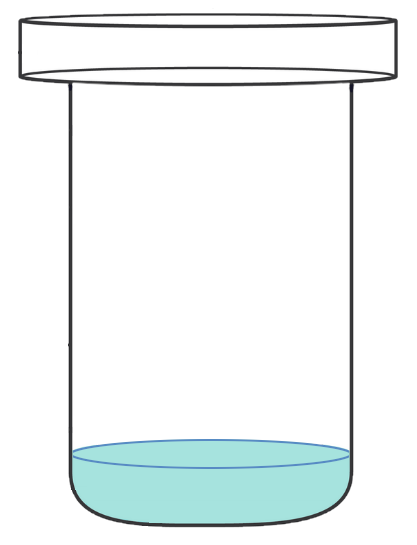
\includegraphics[height=0.15\textheight]{images/chimie/CCM/CCM_etapes_cuve.png}
    \end{center}
    
    \vspace*{-12pt}
    Remplir jusqu'à environ 0,5 cm de hauteur d'éluant la cuve à CCM.
  }{
    \begin{center}
      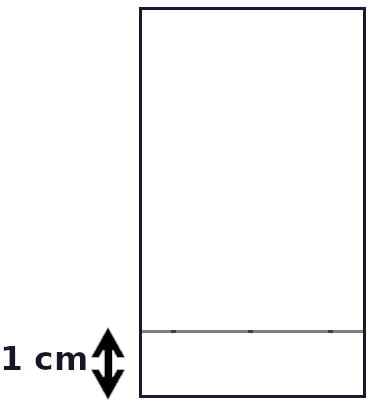
\includegraphics[height=0.15\textheight]{images/chimie/CCM/CCM_etapes_trait.png}
    \end{center}
    
    \vspace*{-12pt}
    À environ 1 cm du bord inférieur, tracer au crayon à papier un trait fin.
    Vérifier que le trait est au-dessus du niveau de l'éluant.
  }{
    \begin{center}
      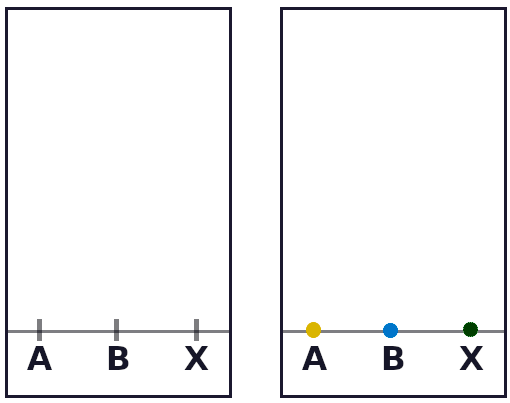
\includegraphics[height=0.15\textheight]{images/chimie/CCM/CCM_etapes_depot.png}
    \end{center}
    
    \vspace*{-12pt}
    Marquer les emplacements des échantillons à déposer.
    Prélever chaque échantillon avec un cure dent et les déposer sur l'emplacement prévu.
  }
  
  \bigskip
  
  \separationBlocs{
    \begin{center}
      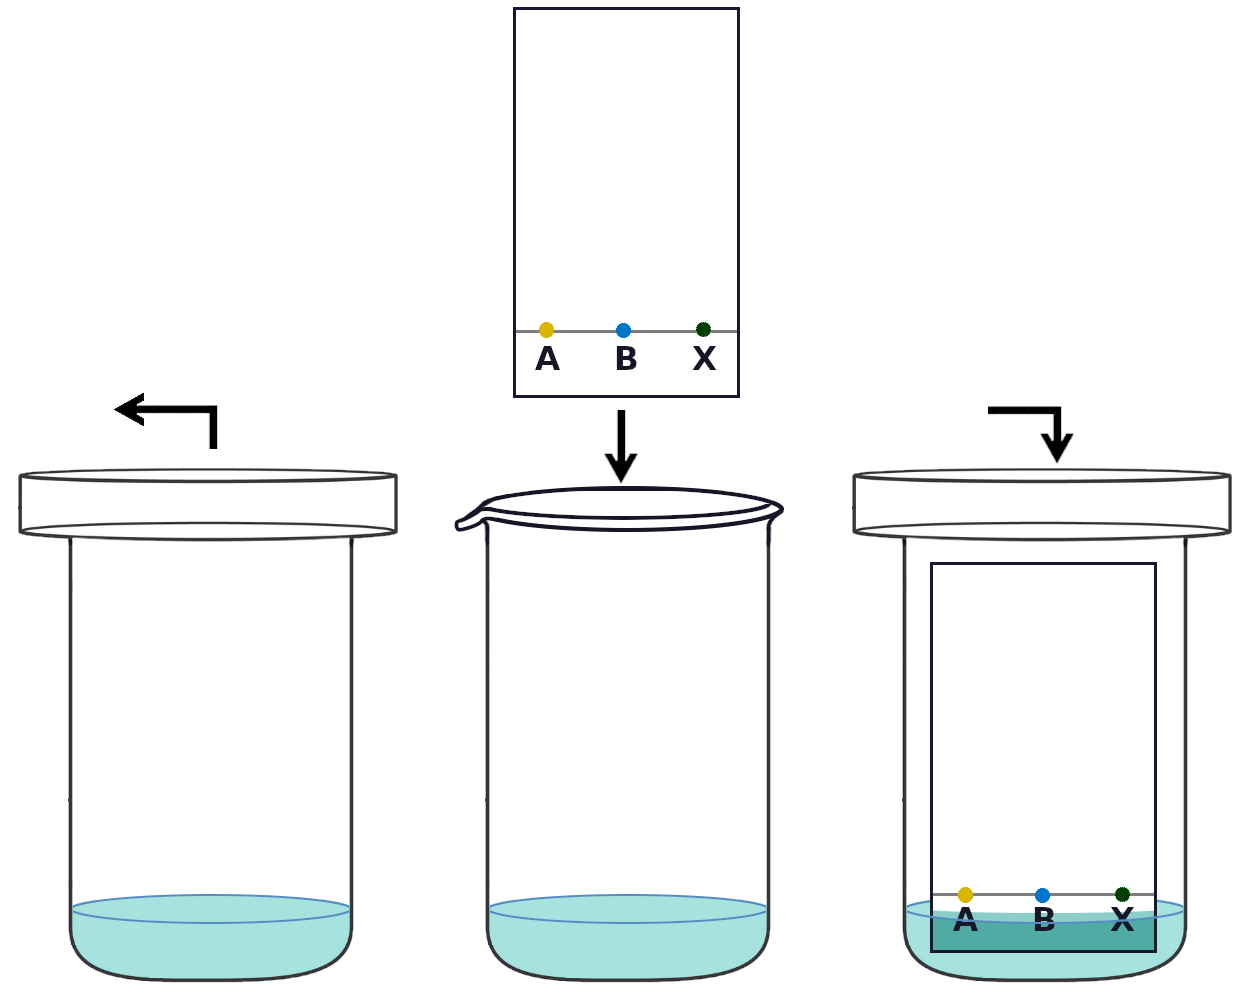
\includegraphics[height=0.25\textheight]{images/chimie/CCM/CCM_etapes_ajout.png}
    \end{center}
    
    \vspace*{-12pt}
    Introduire délicatement la plaque dans la cuve en la tenant par les côtés.
    Refermer la cuve.
    \textbf{Ne jamais déplacer la cuve} et attendre que l'éluant monte.
  }{
    \begin{center}
      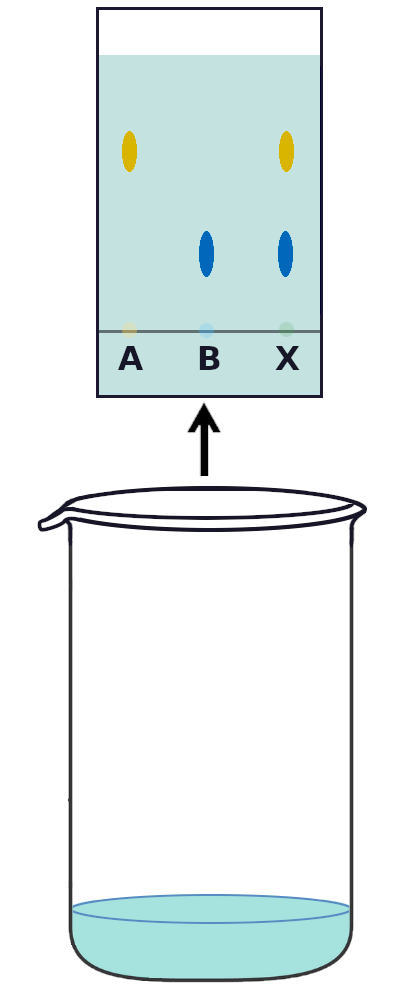
\includegraphics[height=0.25\textheight]{images/chimie/CCM/CCM_etapes_retrait}
    \end{center}
    
    \vspace*{-12pt}
    Quand le front de l'éluant s'approche du bord supérieur, sortir la plaque.
    Tracer immédiatement une ligne indiquant la hauteur où l'éluant est monté.
  }
\end{doc}


%%%% questions
\question{
  Placer quelques gouttes de sirop vert dans un bécher de $50\unit{mL}$. Ajouter environ $10\unit{mL}$ d'eau distillée et agiter.\competence{REA}
}{}{0}

\question{
  Réaliser le protocole du document 3, avec un dépôt de colorant jaune, un dépôt de colorant bleu et  et un dépôt de la solution préparée à la question 1.\competence{REA}
}{}{0}

\question{
  Coller ici le chromatogramme \textbf{sec} et entourer les différentes tâches au crayon à papier.\competence{REA}
}{}{0}
\vspace*{240pt}

\question{
  Pourquoi doit-on placer la ligne de dépôt au dessus du niveau de l'éluant ?\competence{ANA/RAI}
}{}{2}

\question{
  Pourquoi ne doit-on pas déplacer la cuve pendant la montée de l'éluant ?\competence{ANA/RAI}
}{}{2}

\question{
  En analysant le chromatogramme à l'aide du document 2, indiquer si les échantillons sont des corps purs ou des mélanges.\competence{APP}
}{}{3}

\question{
  En utilisant le chromatogramme, que contient le colorant vert du sirop ? Justifier avec des arguments simples.\competence{APP, VAL}
}{}{2}
  % %%%%
\teteSndCorp

%%%% titre
%\vspace*{-36pt}
\numeroActivite{2}
\titreActivite{Mesure de la masse volumique de l'air}


%%%% objectifs
\begin{objectifs}
  \item Calculer la masse volumique de l'air.
\end{objectifs}

\begin{contexte}
  L'atmosphère est un mélange de plusieurs gaz : dioxygène, diazote, dioxyde de carbone, etc.
  
  \problematique{
    Comment calculer la masse volumique de l'air à partir de sa composition ou d'une expérience ?
  }
\end{contexte}


%%%% docs
\begin{doc}{Mesure de la masse volumique de l'air}{doc:A2_masse_volumique_air}
  \begin{wrapfigure}{r}{0.1\linewidth}
    \vspace*{-29pt}
    \qrcode{https://www.youtube.com/watch?v=isEo51ncsKU&t=26s}
  \end{wrapfigure}
  On peut mesurer la masse volumique de l'air en dégonflant un ballon dans une bouteille d'eau.
  La bouteille d'eau permet de mesurer le volume d'air expulsé.
  En pesant le ballon avant et après le dégonflage, on peut calculer la masse d'air expulsée.
\end{doc}

\numeroQuestion 
Schématiser les 3 étapes de l'expérience réalisée.
\vspace*{200pt}

\numeroQuestion
Remplir le tableau ci-dessous 
\begin{tableau}{|c |c |c |c |}
  Grandeur & Masse du ballon plein $m_1 $ & Masse du ballon dégonflé $m_2$ & Volume d'air expulsé $V$ \\
  \SetCell{couleurPrim!10} Valeur & \vphantom{$\dfrac{1}{2}$} & &
\end{tableau}

\question{
  Calculer la masse volumique mesurée $\rho_\text{mes}(\text{air})$.
}{}{3}

%%
\begin{doc}{Masse volumique d'un mélange}{doc:A2_composition_atmo}
  Pour un mélange de gaz, la masse volumique du mélange est simplement la somme des masses volumique de chaque gaz pondérée par la fraction volumique de chaque gaz du mélange.

  Pour l'air, on aura donc
  \begin{equation*}
    \rho(\text{air}) = p_v(\chemfig{O_2}) \rho(\chemfig{O_2}) + p_v(\chemfig{N_2}) \rho(\chemfig{N_2}) + p_v(\chemfig{Ar}) \rho(\chemfig{Ar}) + p_v(\chemfig{CO_2}) \rho(\chemfig{CO_2})
  \end{equation*}
\end{doc}

\newpage
\question{
  Rappeler les fractions volumique des gaz composant l'air (\chemfig{O_2}, \chemfig{N_2}, \chemfig{CO_2}, \chemfig{Ar}).
}{}{2}

\begin{doc}{Masse volumique des gaz composant l'air}{doc:A2_masse_volumique_air}
  \textbf{Données :}
  \begin{listeTirets}
    \item Masse volumique du \chemfig{CO_2} gazeux : $\rho(\chemfig{CO_2}) = \qty{1,87}{\g/\litre}$.
    \item Masse volumique du \chemfig{O_2}  gazeux : $\rho(\chemfig{O_2})  = \qty{1,35}{\g/\litre}$.
    \item Masse volumique du \chemfig{N_2}  gazeux : $\rho(\chemfig{N_2})  = \qty{1,18}{\g/\litre}$.
    \item Masse volumique de \chemfig{Ar}   gazeux : $\rho(\chemfig{Ar})   = \qty{1,78}{\g/\litre}$.
  \end{listeTirets}
\end{doc}


%%%%
\question{
  Calculer la masse volumique théorique de l'air $\rho_\text{theo}(\text{air})$.
}{
}{4}

\question{
  Comparer la valeur théorique et la valeur mesurée. Est-ce qu'elles sont égales ? Est-ce qu'elles sont cohérentes ?
}{}{2}
  %% Chapitre 2
  % %%%% début de la page
\teteSndSolu

%%%% titre
\vspace*{-36pt}
\numeroActivite{1}
\titreTP{Dosage du sucre par étalonnage}

%%%% objectifs
\begin{objectifs}
  \item Apprendre le vocabulaire sur les solutions.
  \item Comprendre la notion de concentration massique
  \item Comprendre le principe de la dilution et de la dissolution
\end{objectifs}


%%%% contexte
\begin{contexte}
  Le sucre couramment présent dans notre alimentation est le saccharose.
  Cette espèce chimique peut entraîner des risques pour la santé si on en consomme trop.
  Il est donc important de pouvoir déterminer la quantité de sucre consommée par jour.

  \problematique{Comment déterminer la masse de saccharose présent dans un sirop ?}
\end{contexte}


%%%% documents
\begin{doc}{Solution, solvant et soluté}{doc:TP1_solution}
  \begin{encart}
    \chevron Une \important{solution} est un mélange homogène. \\
    Le \important{solvant} est le composant majoritaire du mélange.
    Les \important{solutés} sont les espèces qui sont dispersées dans le solvant.
  \end{encart}
  
  \begin{center}
    \important{Solvant + Soluté(s) = Solution}
  \end{center}
  
  \begin{encart}
    On parle de \important{solution aqueuse} si le solvant est l'eau \chemfig{H_2 O}.
  \end{encart}
\end{doc}

\begin{doc}{Composition d'un sirop}{doc:TP1_sirop}
  Le constructeur annonce que le sirop est composé d'\textit{eau}, de \textit{sucre} de \textit{jus de citron} et d'\textit{acide citrique} principalement.
\end{doc}


\question{
  Donner le solvant et les solutés présents dans le sirop.
}{}{2}


%%%%
\begin{doc}{Concentration en soluté}{doc:TP1_concentration}
  \begin{encart}
    La \important{concentration massique $\mathbf{c}$} mesure la quantité de soluté présent dans une solution.
    C'est le rapport de la masse $m$ de \textbf{soluté} dissous dans le volume $V$ de la \textbf{solution}
    \begin{equation*}
      c = \frac{m_\text{soluté}}{V_\text{solution}}
    \end{equation*} 
  \end{encart}
  % \attention Il faut bien distinguer \textbf{concentration massique} et \textbf{masse volumique}.
  % La concentration mesure la masse de soluté contenue dans une solution.
  % La masse volumique mesure la masse d'un échantillon contenue dans un volume donné.
\end{doc}


\begin{doc}{Dissolution du sucre dans l'eau}{doc:TP1_protocole_dissolution}
  \begin{protocole}
      \item Peser une masse donnée de sucre avec une balance de précision.
      \item Mettre le sucre dans une fiole jaugée de 50 mL.
      \item Compléter la fiole jaugée jusqu'à mi-hauteur avec de l'eau distillée, agiter.
      \item Compléter jusqu'au trait de jauge avec de l'eau distillée.
      \item Verser le mélange dans un bêcher de 100 mL.
  \end{protocole}
\end{doc}


%%%% questions
\newpage
\vspace*{-28pt}

\mesure
En utilisant le Document~\ref{doc:TP1_protocole_dissolution}, préparer un mélange de \qty{50}{\ml} d'eau et de de sucre.

\mesure
Mesurer et noter la masse volumique du mélange préparé $\rho =$ \texteTrou[0.1]{\qty{0,15}{\g/\ml}}

\question{
  Calculer la concentration massique de sucre dans la solution aqueuse préparé.
}{}{1}


%%%%
\begin{doc}{Mesure de concentration}{doc:TP1_dosage}
  \begin{encart}
    On parle de \important{dosage} quand on mesure la concentration d'une espèce chimique présente dans une solution.
  \end{encart}
  \begin{encart}
    Un \important{dosage par étalonnage} consiste à déterminer la concentration d’une espèce chimique en comparant une grandeur physique caractéristique de la solution, à la même grandeur physique mesurée pour des solutions étalon.
  \end{encart}
\end{doc}
 
\numeroQuestion 
En utilisant le papier millimétré, tracer la masse volumique en fonction de la concentration massique de sucre dans l'eau.

\numeroQuestion
  En déduire la concentration massique de sucre dans la sirop $c_\text{sirop} =$ \texteTrou[0.1]{\qty{0,6}{\g/\ml}}


%%%%
\begin{doc}{Principe d'une dilution}{doc:TP1_principe_dilution}
  \begin{wrapfigure}[5]{r}{0.5\linewidth}
    \vspace*{-48pt}
    \centering
    \begin{multicols}{4}
    \image{1}{images/chimie/protocoles/dilution0001} \\[-12pt]
    \footnotesize{$S_0$}
    
    \image{1}{images/chimie/protocoles/dilution0002}
    
    \image{1}{images/chimie/protocoles/dilution0003}
    
    \image{1}{images/chimie/protocoles/dilution0004} \\[-12pt]
    \footnotesize{$S_1$}
    \end{multicols}
  \end{wrapfigure}
  \vAligne{-40pt}
  
  \begin{encart}
    Le principe de la \important{dilution} est de \important{diminuer la concentration} en soluté dans une solution en rajoutant du \important{solvant.}
  \end{encart}
  La solution de départ est appelée \important{solution mère}, notée $S_0$.
  La solution obtenue après dilution est appelée \important{solution fille}, notée $S_1$.

  Pour diluer une solution, il faut
  \begin{protocole}
    \item Prélever un volume $V_0$ de la solution à l'aide de la pipette graduée.
    Le bas du ménisque doit atteindre la graduation supérieure.
    \item Introduire la solution prélevée dans la fiole jaugée de volume $V_1$.
    \item Ajouter de l'eau distillée dans la fiole jaugée jusqu'aux $2/3$ et agiter doucement. Compléter jusqu'à ce que le bas du ménisque atteigne le trait de jauge.
    \item Fermer la fiole et l'agiter en la retournant plusieurs fois.
    \item Verser la solution fille obtenue dans un bécher.
  \end{protocole}
\end{doc}


%%%%
\begin{doc}{Facteur de dilution}{doc:TP1_dilution}  
  Le \important{facteur de dilution} est le rapport du volume de la solution fille sur le volume de la solution mère
  \begin{equation*}
    F = \frac{V_\text{1}}{V_\text{0}}
  \end{equation*}
  On dit qu'on a dilué $F$ fois une solution.
\end{doc}

\mesure 
Diluer 2 fois le sirop et mesurer sa masse volumique. 

\numeroQuestion
En en déduire la concentration massique en sucre.
Que constatez-vous ?
  % \input{Seconde/C1_corps_melanges/corp1B_dosage_dakin}
  % \input{Seconde/C1_corps_melanges/corp1B_dosage_identification}
  %% Chapitre 3
  % %%%% début de la page
\sndEnTeteDeux

%%%%
\nomPrenomClasse


%%%% titre
\numeroActivite{1}
\titreActivite{Décrire le mouvement}


%%%% objectifs
\begin{objectifs}
  \item Décrire un mouvement.
  \item Comprendre la notion de référentiel.
  \item Comprendre que le mouvement dépend du référentiel.
\end{objectifs}


%%%% evaluation
\begin{tableauCompetences}
  \centering APP &
  Rechercher l'information.
  
  Représenter la situation par un schéma.
  & & & &
  \\ \hline
  \centering ANA/RAI &
  Proposer une stratégie de résolution.
  & & & &
\end{tableauCompetences}

%%%%
\vspace*{6pt}
\begin{doc}{Un peu de vocabulaire}
  \vspace*{-24pt}
  \begin{encart}
    \important{Système} : objet dont on étudie le mouvement.
  \end{encart}
  
  \begin{encart}
    \important{Trajectoire} : ensemble des positions successives occupées par le système.
  \end{encart}
  
  Le \important{mouvement} d'un système est donné par la description de sa trajectoire + l'évolution de sa vitesse.
\end{doc} 


\vspace*{2pt}
\begin{doc}{Type de trajectoires}
  \label{doc:trajectoires}

  Trajectoire \important{rectiligne} : trajectoire représentée par \dotfill \\[4pt]
  Trajectoire \dotfill : trajectoire représentée par un cercle. \\[4pt]
  Trajectoire \important{curviligne} : trajectoire représentée par \dotfill
\end{doc}


\vspace*{2pt}
\begin{doc}{Vitesse et accéleration}
  \label{doc:vitesse}

  Vitesse \important{uniforme} (constante) : le système n’accélère pas. \\[4pt]
  La vitesse augmente : le système \dotfill \\[4pt]
  La vitesse diminue : le système \dotfill \\[4pt]
  Si la vitesse est \dotfill on dit que le système est \important{immobile}.
\end{doc}


%%%%
\newpage

\question{Compléter les documents~\ref{doc:trajectoires} et~\ref{doc:vitesse}.}{0}

\fleche Pour la suite de cette activité, vous allez choisir entre l'étude du mouvement des oies ou de la Lune.
Vous présenterez ensuite les résultats de votre étude au reste de la classe à l'oral.


%%%%
\titreSection{\'Etude du mouvement des oies}

Le compteur du bateau affiche une vitesse $v_\text{bateau} = 3,\!6 \times 10^1 \unit{km/h}$.

\vspace*{6pt}
\question{Pour la personne qui filme les oies, quelle est la vitesse des oies ?}{0}
\question{Pour une personne se trouvant sur la berge, quelle est la vitesse des oies ?}{0}
\question{Schématiser la trajectoire des oies si on les observe depuis la berge.}{0}
\question{Indiquer le mouvement des oies depuis le bateau et la berge.}{0}

\titreSection{\'Etude du mouvement de la Lune}

La Lune tourne autour de la Terre à une vitesse $v_\text{Lune} = 3,\!7 \times 10^3 \unit{km/h}$ et la Terre tourne autour du Soleil à une vitesse $v_\text{Terre} = 1,\!1 \times 10^5 \unit{km/h}$.

\begin{figure}[!ht]
  \begin{subfigure}{0.48\linewidth}
    \centering
    \image{0.8}{images/mouvements/terre_lune.png}
    \caption{Point de vue centré sur la Terre}
    \label{fig:terre_lune}
  \end{subfigure}
  \begin{subfigure}{0.48\linewidth}
    \centering
    \image{0.8}{images/mouvements/terre_lune_soleil.png}
    \caption{Point de vue centré sur le Soleil}
    \label{fig:terre_lune_soleil}
  \end{subfigure}
\end{figure}

\vspace*{-6pt}
\question{Depuis le point de vue centré sur la Terre, quelle est la vitesse de la Lune ?}{0}
\question{Schématiser la trajectoire de la Lune depuis ce point de vue et indiquer son mouvement.}{0}
\question{Peut-on décrire la vitesse de la Lune depuis le point de vue centré sur le Soleil ?}{0}
\question{Schématiser la trajectoire de la Lune depuis ce point de vue.}{0}


\titreSection{Notion de référentiel}

\question{Convertir la vitesse $v_\text{Lune}$ en m/s.
\textit{Rappel : } $1\unit{km} = 10^3\unit{m}$, $1\unit{h} = 3,\!6 \times 10^3 \unit{s}$.}{0}
\question{Quelle distance la Lune parcours pendant 1 seconde ? Comparer avec la longueur de sa trajectoire, qui est de $2,4\times 10^6 \unit{km}$}{0}
\question{Est-ce que la seconde est une durée d'observation suffisante pour décrire la trajectoire de la Lune ?}{0}
\question{Conclusion : pourquoi est-il important de définir le référentiel, qui est l’endroit où on se place et le temps passé à observer, avant d'étudier un mouvement ?}{0}

\feuilleBlanche
  % %%%% début de la page
\sndEnTeteDeux

%%
\nomPrenomClasse


%%%% titre
\numeroActivite{2}
\titreActivite{Chute d'une balle}


%%%% objectifs
\begin{objectifs}
  \item Comprendre la notion de vecteur vitesse.
  \item Tracer des vecteurs vitesses.
\end{objectifs}


%%%% evaluation
\begin{tableauCompetences}
  \centering S'Approprier (APP) &
  Représenter la situation par un schéma.
  & & & &
  \\ \hline
  \centering Communication (COM) &
  Travailler en groupe, échanger entre élèves.
  & & & &
\end{tableauCompetences}


%%
\vspace*{6pt}
\problematique{Quelle est l'influence d'une translation sur la description du mouvement d'un objet ?}


%%%% documents
\begin{doc}{Chronophotographie de la chute d'une balle}
  \label{doc:chrono}
  \vspace*{-20pt}
  \begin{center}
    \image{0.9}{images/mouvements/chronophotographie_balle.png}
  \end{center}
  Une chronophotographie est une superposition de plusieurs images prises les unes après les autres avec un intervalle de temps régulier.
  Pour réaliser cette chronophotographie, \textbf{on a pris une image toutes les} $\mathbf{40} \unit{\mathbf{ms}}$.
  \bigskip
  
  Réaliser une chronophotographie permet de repérer des positions par lesquelles passent la balle, ce qui est impossible à l'oeil nu.
  Les ronds indiquent les positions de la balle, les carrés indiquent les positions du centre de masse de l'homme sur la trottinette.
\end{doc}

%%
\begin{doc}{Vecteur}
  \label{doc:vecteur}
  \vspace*{-24pt}
  \begin{encart}
    \important{Vecteur} : objet mathématique représenté par un segment fléché $\longrightarrow$ et noté avec une lettre surmontée d'une flèche $\vv{v}$.
    
    Un vecteur contient quatre information : une \important{direction}, un \important{sens}, une \important{norme,} et un \important{point d'application} (ou origine).
  
    Un vecteur est \important{constant} si sa direction, son sens et sa norme ne varie pas le long du mouvement.
  \end{encart}
\end{doc}

%%
\begin{doc}{Vecteur déplacement et vecteur vitesse d'un point}
  \label{doc:vitesse}
  Soient $P_1$ la position d'un point à l'instant $t_1$ et $P_3$ la position de ce même point à l'instant $t_3$.
  Le déplacement du point matériel entre les dates $t_1$ et $t_3$ est défini par le vecteur déplacement $\vv{P_1 P_3}$.
  Graphiquement, c'est la flèche qui relie $P_1$ à $P_3$. 
  \bigskip
  
  Le vecteur $\vv{P_1 P_3}$ est caractérisé par
  \begin{listePoints}
    \item une direction : celle de la droite $P_1 P_3$.
    \item Un sens : de $P_1$ vers $P_2$.
    \item Une norme : égale à la distance $P_1 P_3$ en mètre (m).
    \item Une origine : le point $P_1$
  \end{listePoints}
  
  \begin{encart}
    Le \important{vecteur vitesse} $\vv{v_2}$ d'un système au point $P_2$ entre les instants $t_1$ et $t_3$ a pour expression
    \begin{equation}
      \vv{v_2} = \frac{\vv{P_1 P_3}}{t_3 - t_1}
    \end{equation}
  \end{encart}
  
  Le vecteur $\vv{v_2}$ est caractérisé par :
  \begin{listePoints}
    \item une direction : parallèle au segment $P_1 P_3$ et tangent à la trajectoire.
    \item Un sens : le sens du mouvement.
    \item Une norme : $v_2 
    = \norm{\vv{v_2}}
    = \displaystyle \norm{\frac{\vv{P_1 P_3}}{t_3 - t_1}}
    = \displaystyle \frac{P_1 P_3}{t_3 - t_1}$.
    \item Une origine : $P_2$.
  \end{listePoints}
  $P_1 P_3$ est la distance entre les points $P_1$ et $P_3$ en mètre (m). $t_3 - t_1$ est la durée séparant les instants $t_1$ et $t_3$ en seconde (s). $v_2$ est la norme de la vitesse en mètre par seconde (m/s).
\end{doc}



%%%%
\newpage
\titreSection{Mouvement dans le référentiel de \lignePointillee{0.2}}

%
\exo{
  Quel est le référentiel utilisé pour décrire le mouvement de la balle et de l'homme sur la trottinette ici ?
}{1}


%%
\titreSousSection{Mouvement de l'homme sur la trottinette}

%
\exo{
  Quelle est la trajectoire de l'homme sur la trottinette ?
}{1}

%
\exo{
  Comment évolue la vitesse de l'homme sur la trottinette ? Indiquer la nature de son mouvement.
}{2}


%%%%
\titreSousSection{Mouvement de la balle}

%
\exo{
  Repérer sur la chronophotographie du document~\ref{doc:chrono}, le point de départ de la balle.
  On notera $P_1$ cette position.
  Numéroter les positions successives de la balle, que l'on notera $P_2, P_3, \ldots P_8$
}{0}

%
\exo{
  Tracer sur la photo du document~\ref{doc:chrono} le vecteur $\vv{P_2 P_3}$ et le vecteur $\vv{P_5 P_7}$.
}{0}

%
\exo{
  En utilisant l'échelle sur la photo, déterminer les normes en mètre de ces deux vecteurs.
  Indiquer si ces normes sont identiques.
}{2}

%
\exo{
  Calculer la norme en mètre par seconde de ces deux vecteurs, en vous aidant du document~\ref{doc:vitesse}.
}{2}

%
\exo{
  Schématiser le vecteur vitesse $\vv{v_2}$ entre les points $P_2$ et $P_3$ et le vecteur vitesse $\vv{v_6}$ entre les points $P_5$ et $P_7$, en vous aidant du document~\ref{doc:vitesse}.
}{0}

\feuilleBlanche

%%%%
% \newpage
% \titreSection{Mouvement dans le référentiel de la trottinette}
% 
% %
% \exo{
%   Ouvrir la vidéo de la de chute balle dans le logiciel Tracker.
% }{0}
% 
% %
% \exo{
%   Repérer dans la vidéo le moment où la balle commence à tomber. 
% }{0}
% 
% %
% \exo{
%   Sur la vidéo, réaliser le pointage de la balle.
% }{0}
% 
% %
% \exo{
%   Tracer la norme de la vitesse, la vitesse selon l'axe $x$ et la vitesse selon l'axe $y$.
%   Que remarquez vous pour la vitesse selon l'axe $x$ ?
% }{2}
% 
% %
% \exo{
%   Que pouvez-vous en déduire sur la nature du mouvement de la balle dans le référentiel de la trottinette ?
%   Représenter avec un schéma sa trajectoire.
% }{2}
% \vspace{200pt}
% 
% %
% \exo{
%   Conclure sur la position de la balle au moment où elle touche le sol par rapport à la trottinette.
% }{2} % 2 séances
  % %%%% début de la page
\sndEnTeteDeux

%%
\nomPrenomClasse


%%%% titre
\numeroActivite{3}
\titreActivite{Modéliser le mouvement}


%%%% objectifs
\vspace{-10pt}
\begin{objectifs}
  \item Comprendre les limites du modèle du point matériel.
  \item Comprendre la notion de référentiel.
  \item Comprendre la notion de vecteur.
\end{objectifs}


%%%% evaluation
\begin{tableauCompetences}
  \centering Communication (COM) &
  Travailler en groupe, échanger entre élèves.
  & & & &
\end{tableauCompetences}


%%%%
\titreSection{Système et référentiel}

%%%%
\vspace{-10pt}
\begin{doc}{Modèle du point matériel}
  \vspace*{-24pt}
  \begin{encart}
    \important{Système} : objet dont on étudie le mouvement.
  
    On ne va s'intéresser qu'au mouvement global du système.
    C'est pourquoi on va modéliser le système par \dotfill \\[8pt]
    \reponse{1}
    \vspace*{-12pt}
    %un point de même masse, localisé en son centre de masse.
    %C'est le \important{modèle du point matériel}.
  \end{encart}

  \fleche Le modèle du point matériel revient à oublier toute information sur la géométrie du système étudié. 
  Les éventuelles rotations et déformations ne sont donc pas prises en compte.
\end{doc}


\begin{tabularx}{\linewidth}{ m{0.2\linewidth} | m{0.2\linewidth} | m{0.25\linewidth} | m{0.26\linewidth} }
  \rowcolor{gray!20}
  \centering Système & Centre de masse & \centering Trajectoire & Informations perdues
  \\ \hline
  %
  \centering
  \phantom{\small b} \newline
  \image{0.8}{images/mouvements/point_balle_tennis.png}
  \newline
  Balle de tennis &
  \centering Centre de la balle & &
  \\ \hline
  %
  \centering
  \phantom{\small b} \newline
  \image{0.8}{images/mouvements/point_roue.jpg} \newline
  Roue &
  \centering Centre de la roue & &
  \\ \hline
\end{tabularx}
\newpage

\vspace*{-30pt}
\begin{tabularx}{\linewidth}{ m{0.2\linewidth} | m{0.2\linewidth} | m{0.25\linewidth} | m{0.3\linewidth} }
  \hline
  %
  \centering
  \phantom{\small b} \newline
  \image{0.8}{images/mouvements/point_humain_course.jpg}
  \newline
  Modèle d'humain &
  \centering Nombril & &
  \\ \hline
\end{tabularx}

%%
\begin{doc}{Référentiel}
  Pour décrire le mouvement, il faut pouvoir le repérer dans l’espace et dans le temps, pour ça on utilise un référentiel.
  
  \begin{encart}
    \important{Référentiel} : objet de référence, muni d'un \dotfill, \newline
    par rapport auquel on étudie le mouvement du système.
  \end{encart}
  
  \begin{encart}
    La description du mouvement dépend du \important{référentiel} choisi. On appelle ça la \important{relativité} du mouvement.
  \end{encart}
\end{doc}


%%%%
\titreSection{Vecteur}

%%
\begin{doc}{Vecteur en physique}
  \label{doc:vecteur}
  \vspace*{-24pt}
  \begin{encart}
    \important{Vecteur} : objet mathématique représenté par un segment fléché $\longrightarrow$ et noté avec une lettre surmontée d'une flèche $\vv{v}$.
    
    Un vecteur contient quatre information : 
    \begin{listePoints}
      \item \dotfill
      \item \dotfill 
      \item \dotfill 
      \item \dotfill 
    \end{listePoints}
  
    Un vecteur est \important{constant} si \dotfill  \\[8pt]
    \reponse{1}
    \vspace{-8pt}
  \end{encart}
  
  \fleche En physique on va se servir des vecteurs pour représenter différentes quantités : \\[8pt]
  \reponse{1}
  
  \attention Un vecteur n'est \textbf{jamais} égal à un nombre, qui contient moins d'information.
\end{doc}
  % %%%% début de la page
\teteSndMouv

%%
\nomPrenomClasse


%%%% titre
\numeroActivite{4}
\titreActivite{Modéliser une action}


%%%% objectifs
\vspace{-10pt}
\begin{objectifs}
  \item Comprendre la notion de force
  \item Connaître la force d'interaction gravitationnelle
  \item Comprendre le lien entre la force d'interaction gravitationnelle et le poids
\end{objectifs}


%%%% evaluation
\begin{tableauCompetences}
  \centering Communication (COM) &
  Travailler en groupe, échanger entre élèves.
  & & & &
\end{tableauCompetences}


%%%%
\titreSection{Système et référentiel}

%%%%
\vspace{-10pt}
\begin{doc}{Satellite Hubble}{doc:satellite_hubble}
  \begin{wrapfigure}{l}{0.4\linewidth}
    \image{1}{images/mouvements/hubble}
  \end{wrapfigure}
  
  Le satellite Hubble est un satellite de masse $m_S = 1,\!1 \times 10^4 \unit{kg}$ conçu par la NASA avec une  participation de l'Agence spatiale européenne, l'ESA.
  
  Ce satellite est opérationnel depuis 1990 et tourne autour de la Terre en 96 min.
  Vu depuis le centre de la Terre, il a un mouvement circulaire uniforme autour de la Terre, à une altitude $h = 590 \unit{km}$.
  
  Ce satellite contient un télescope qui permet d’observer les étoiles et objets de l’univers depuis l’espace !
\end{doc}

%%
\begin{doc}{Force et action mécanique}{doc:force_action_mecanique}
  \chevron Un corps exerce une \important{action mécanique} sur le système étudié si \reponseLigne
  \reponseLigne{1}
  
  Pour modéliser une action mécanique, on utilise le concept de \important{force}.
  
  \begin{encart}
    La force exercée par un corps $A$ sur un corps $B$ est représentée par un vecteur $\vvFAsurB$.
    Ce vecteur possède les caractéristiques suivantes :
    \begin{listePoints}
      \item Une \important{norme} notée $\FAsurB$, qui s'exprime en \dotfill
      \item Une \important{direction} et un \important{sens} qui dépendent de la situation.
      \item Un \important{point d'application} : le centre du système $B$.
    \end{listePoints}
  \end{encart}
\end{doc}

%%
\newpage
\begin{doc}{Force d'interaction gravitationnelle}{doc:interaction_gravitationnelle}
  \chevron Tous les corps qui possèdent une masse s’attirent entre eux : c’est l’attraction gravitationnelle.

  \begin{encart}
    On modélise l'attraction gravitationnelle exercée par le corps $A$ sur le corps $B$ par une force représentée par un vecteur $\vvFAsurB$ :
    
    \vspace*{-12pt}
    \begin{wrapfigure}[6]{r}{0.4\linewidth}
      \vspace*{-20pt}
      \begin{tikzpicture}
        % corps A et B
        \tkzCercle{0}{0}{gray!50!white}{20}
        \tkzLabel{-1.2}{0}{$m_A$}
        \tkzCercle{4}{2}{gray!50!white}{20}
        \tkzLabel{2.8}{2}{$m_B$}
        \tkzPointLabel{0}{0}{$A$}
        \tkzPointLabel{4}{2}{$B$}
        % force et distance
        \tkzVecteur{4}{2}{-1.5}{-0.75}{$\vvFAsurB$}{left}
        \tkzEquiv{0.5}{-1}{4}{2}{\phantom{G}$d$}{right}
      \end{tikzpicture}
    \end{wrapfigure}

    \phantom{b}
    \begin{listePoints}
      \item \important{Point d'application} : centre du corps $B$
      \item \important{Direction} : la droite $AB$.
      \item \important{Sens} : de $B$ vers $A$ (force attractive).
      \item \important{Norme} : $\FAsurB = \ldots\ldots\ldots$
    \end{listePoints}
      
    Dans la formule de la norme de la force, les masses s'expriment en kilogramme (kg), la distance en mètre (m) et la \important{constante universelle de gravitation} $G$ en newton mètre carrée par kilogramme carrée ($\!\!\unit{N \cdot m^2 \cdot kg^{-2}}$). Sa valeur (à connaître) est 
    \begin{equation*}
      G = \ldots\ldots\ldots\ldots
      %6,67 \times 10^{-11}
      \unit{N \cdot m^2 \cdot kg^{-2}}
    \end{equation*}
  \end{encart}
\end{doc}

%%%%
\question{
  Compléter les documents \ref{doc:force_action_mecanique} et \ref{doc:interaction_gravitationnelle}.
}{

}{0}

\question{
  Donner trois exemples d'actions mécaniques qu'on peut rencontrer dans la vie quotidienne.
}{

}{5}

\question{
  Quelle différence remarquez-vous entre ces actions de la vie quotidienne et l'action exercée par la Terre sur le satellite Hubble ?
}{

}{3}

\question{
  Sur le schéma ci-dessous, représenter la force d’interaction gravitationnelle F T /S exercée par la Terre T sur le satellite Hubble S.
  La Terre est assimilée à une boule de rayon $R_T = \qty{6,37e3}{\km}$ et de masse $M_T = \qty{5,97e24}{\kg}$.
}{
  bla
}{0}

\question{
   En utilisant le document 3, donner la relation qui relie la norme de la force FT/S et la masse du satellite $m_S$, la masse de la Terre $M_T$, la constante G et la distance d.
}{

}{2} % 2 séances
  % %%%% début de la page
\sndEnTeteDeux


%%%% titre
\numeroActivite{5}
\titreActivite{Mouvement et forces}


%%%% objectifs
\begin{objectifs}
  \item Comprendre la notion de force, connaître des exemples de forces
  \item Comprendre le lien entre mouvement et force
  \item Comprendre le principe d'inertie
\end{objectifs}
\bigskip


%%%%
\begin{doc}{Force et action mécanique}
  \label{doc:action_force_comp}
  \chevron Un corps exerce une \important{action mécanique} sur le système étudié s’il est capable d’en modifier le mouvement.
  Une action mécanique est modélisée par une \important{force.}

  \begin{encart}
    La force exercée par un corps $A$ sur un corps $B$ est représentée par un vecteur $\vvFAsurB$.
    Ce vecteur possède les caractéristiques suivantes :
    \begin{listePoints}
      \item Une \important{norme} notée $\FAsurB$, qui s'exprime en newton (N).
      \item Une \important{direction} et un \important{sens} qui dépendent de la situation.
      \item Un \important{point d'application} : le centre du système $B$.
    \end{listePoints}
  \end{encart}
\end{doc}
\bigskip

%%
\begin{doc}{Exemples de forces}
  \label{doc:exemples_forces}
  On distingue 2 types d'actions : les \important{actions de contact} (contact entre l’objet qui donne la force et l’objet qui la reçoit), et les \important{actions à distance} (pas de contact).
  \smallskip
  
  \begin{tabularx}{\linewidth}{| m{0.3\linewidth} | m{0.275\linewidth} | m{0.35\linewidth} |}
    \hline
    \rowcolor{gray!20}
    \centering Force &
    \centering Norme &
    Direction, sens 
    \\ \hline
    %
    \centering poids $\vv{P}$ &
    \centering $P = m \times g$ &
    verticale, vers le bas
    \\ \hline
    %
    \centering réaction du support $\vv{R}$ &
    \centering égale à celle du poids : \newline $R = P$ &
    perpendiculaire au support, vers le haut
    \\ \hline
    %
    \centering frottements $\vv{f}$ &
    dépend du cas étudié &
    $\vv{f}$ est opposée à la vitesse $\vv{v}$ (opposée au mouvement)
    \\ \hline
  \end{tabularx}
  \smallskip
  
  \begin{listePoints}
    \item Le poids $\vv{P}$ représente l'interaction gravitationnelle de la Terre.
    \item La réaction du support $\vv{R}$ représente l'action exercée par le support sur un objet posé dessus.
    \item Les frottements $\vv{f}$ représentent l'action d'un milieu (gaz, liquide, support solide) sur un objet qui s'y déplace.
  \end{listePoints}
\end{doc}

%%%%
\begin{tabularx}{\linewidth}
{| m{0.2\linewidth} | m{0.37\linewidth} | m{0.36\linewidth} |}
  \hline
  %
  \rowcolor{gray!20}
  \centering
  Système &
  Ballon &
  Curling
  \\ \hline
  %
  Forces appliquées &
  \phantom{\small b} \newline
  \image{1}{images/mouvements/ballon_football} &
  \phantom{\small b} \newline
  \image{1}{images/mouvements/curling}
  \\ \hline
  %
  \centering Mouvement &
  \centering Immobile &
  \phantom{b} \newline
  \\ \hline
  %
  \rowcolor{gray!20}
  \centering
  Système &
  Parachutiste &
  Skieuse
  \\ \hline
  %
  Forces appliquées &
  \phantom{\small b} \newline
  \image{1}{images/mouvements/parachutiste} &
  \phantom{\small b} \newline
  \image{1}{images/mouvements/skieur}
  \\ \hline
  %
  \centering Mouvement &
  &
  \phantom{b} \newline
  \\ \hline
\end{tabularx}

\begin{figure}[!ht]
  \caption{Représentation des forces pour quelques situations sportives}
  \label{tab:situations_sportives}
\end{figure}


%%%%
\newpage
\vspace*{-36pt}
\titreSection{Forces et mouvement}

%%
\question{
  Parmi les forces $\vv{P}$, $\vv{R}$ et $\vv{f}$, indiquer celles qui sont des forces de contact et celles qui sont des forces à distance.
}{3}

\question{
  En vous aidant des documents~\ref{doc:action_force_comp} et~\ref{doc:exemples_forces}, compléter la figure~\ref{tab:situations_sportives} :
}{0}

\vspace*{-6pt}
\sousQuestion{Sur chaque système étudié, schématiser avec des flèches la ou les forces entrant en jeu, en faisant attention à son point d'application.}{0}

\vspace*{-6pt}
\sousQuestion{Pour chaque système, indiquer son mouvement pour un ou une observatrice extérieure (trajectoire + évolution de la vitesse).}{0}


%%%%
\titreSection{Principe d'inertie}

\question{
  Répondre par vrai ou faux en justifiant à l'aide d'exemples ou de contre exemples.
}{0}

\vspace*{-6pt}
\sousQuestion{Si un objet est en mouvement, alors il est forcément accéléré.}{2}

\sousQuestion{Si un objet est en mouvement, alors il subit une force dans le sens du mouvement.}{2}

\sousQuestion{Si deux objets sont animés par les mêmes forces, alors ils suivent la même trajectoire.}{2}

\question{
  On dit que deux forces se compensent si leur sommes vectorielle est nulle.
  Pour quels systèmes de la figure~\ref{tab:situations_sportives} les forces se compensent-elles ?
}{2}

\question{
  Quel est le mouvement du système dans chaque cas où les forces se compensent ?
}{2}



\begin{doc}{Conclusion : Le principe d'inertie}
  \phantom{b}
  \vspace*{-12pt}
  
  \chevron Le \important{principe d'inertie} a été formulé pour la première fois par Newton en 1687.
  Newton s'appuyait sur les travaux de Descartes et de Galilée, et parfois on appelle ce principe la \important{première loi de Newton}.
  Sa formulation moderne est la suivante :
  
  \begin{encart}
    Si les forces qui s'exercent sur un système se compensent, alors ce système est \\[6pt]
    soit \lignePointillee{0.2}, 
    soit en mouvement \dotfill
  \end{encart}
  
  \begin{encart}
    Réciproquement, si un système est \dotfill \\[6pt]
    .\dotfill, alors les forces\\[6pt]
    . \dotfill
  \end{encart}
\end{doc}


%%%%
\titreSection{Variation du vecteur vitesse}

\question{
  Comment varie $\vv{v}$ pour un système qui a un mouvement rectiligne uniforme ?
  En déduire la variation de $\vv{v}$ pour un système soumis à des forces qui se compensent.
}{3}

\begin{doc}{Principe d'inertie et vitesse}
  \vspace*{-24pt}
  \begin{encart}
    Le principe d'inertie dit que si le vecteur vitesse \dotfill \\[6pt]
    au cours de la trajectoire, alors \dotfill \\[6pt]
    \reponse{1}
    %les forces exercées sur le système se compensent.
  \end{encart}
\end{doc} % 3 séances
  % %%%% début de la page
\sndEnTeteDeux

%%
\nomPrenomClasse


%%%% titre
\numeroActivite{6}
\titreActivite{Principe des actions réciproques}


%%%% evaluation
\vspace*{-8pt}
\begin{tableauCompetences}
  %
  \centering ANA/RAI &
  Analyser les forces qui s'exercent sur un système.
  & & & &
  \\ \hline
  %
  \centering REA &
  Schématiser une situation.
  & & & &
  \\ \hline
  %
  \centering COM &
  Travailler en groupe.
  & & & &
\end{tableauCompetences}


%%%% objectifs
\begin{objectifs}
  \item Analyser et schématiser un système en mouvement
  \item Comprendre le principe des actions réciproques
\end{objectifs}


%%%%
\begin{doc}{Forces qui se compensent}
  \vspace*{-22pt}
  \begin{encart}
    On dit que les forces exercées sur un système \important{se compensent}, si leur somme vectorielle est nulle (égale à $\vv{0}$ le vecteur de norme nulle).
    
    La somme de deux vecteurs est nulle s'ils ont
    
    \begin{wrapfigure}[1]{r}{0.5\linewidth}
      \vspace*{-55pt}
      \begin{center}
        \begin{tikzpicture}
          % système 
          \tkzCercle{0}{0}{gray!50!white}{20}
          \tkzPointLabel{0}{0}{$A$}
          % forces
          \tkzVecteur{0}{0}{-1.7}{-0.75}{$\vv{F}_1$}{left}
          \tkzVecteur{0}{0}{1.7}{0.75}{$\vv{F}_2$}{right}
        \end{tikzpicture}
      
        $\vv{F}_1 + \vv{F}_2 = \vv{0}$, les forces exercée sur le système $A$ se compensent.
      \end{center}
    \end{wrapfigure}
    \phantom{b} 
    
    \vspace*{-24pt}
    \begin{listePoints}
      \item \important{même point d'application},
      \item \important{même direction},
      \item \important{même norme},
      \item mais des \important{sens opposés}.
    \end{listePoints}
  \end{encart}
\end{doc}


%%%%
\begin{doc}{\href{https://www.youtube.com/watch?v=Kf0bBxmNeec}{Ballon lancé depuis un skateboard}}
  \vspace*{-22pt}
  \begin{center}
    \image{0.31}{images/mouvements/lancer_balle_reciproque_1.jpg}
    \image{0.31}{images/mouvements/lancer_balle_reciproque_2.jpg}
    \image{0.31}{images/mouvements/lancer_balle_reciproque_3.jpg}
  \end{center}
\end{doc}


%%%
\problematique{Quelle est la force qui met en mouvement la personne sur le skateboard ?}

\question{
  Étudier le mouvement du système $A$ \og personne sur le skateboard \fg\; et du système $B$ \og ballon \fg\; avant, pendant et après le lancé du ballon.
}{0}
\vspace*{-8pt}
\question{
  Décrire les propriétés de la force qui met en mouvement le système $A$.
}{0}

\fleche Détaillez soigneusement les étapes de vos raisonnements par écrits au dos de cette feuille.

\feuilleBlanche
  % %%%% début de la page
\sndEnTeteDeux

%%
\nomPrenomClasse


%%%% titre
\numeroActivite{7}
\titreActivite{Chute d'une goutte d'encre}


%%%% evaluation
\begin{tableauCompetences}
  %
  \centering APP &
  Analyser un programme python.
  & & & &
  \\ \hline
  %
  \centering REA &
  Mesurer des positions avec un logiciel de pointage.
  & & & &
  \\ \hline
  %
  \centering COM &
  Travailler en groupe.
  & & & &
\end{tableauCompetences}


%%%% objectifs
\begin{objectifs}
  \item Utiliser des outils numériques pour analyser un mouvement.
\end{objectifs}


%%%%
\begin{doc}{Mesurer les positions avec Cineris}
  \label{doc:cineris}
  Pour mesurer les positions d'un objet, dans Cineris il faut cliquer sur :
  \begin{enumeration}
    \item \texttt{Montage} (1), puis \texttt{choix du fichier} et ouvrir \url{chute_goutte.avi}.
    \item Cliquer sur \texttt{Traitement manuel} (2) puis sur \texttt{étalonnage} (3)
    \begin{listePoints}
      \item maintenir appuyé le clic-gauche de la souris sur la vidéo
      \item glisser verticalement le long d'un objet de référence et relâcher pour régler l'échelle verticale.
    \end{listePoints}
    \item Cliquer sur le bouton vert dans \texttt{traitement} (4), puis 
    \begin{listePoints}
      \item cliquer sur le centre de l'objet pour mesurer sa position ;
      \item répéter pour chaque instants de la vidéo ;
      \item appuyer sur le bouton rouge pour arrêter le traitement.
    \end{listePoints}
    \item Cliquer sur \texttt{Tableau} (5) pour accéder aux positions mesurée.
  \end{enumeration}
  
  \centering
  \image{0.6}{images/logiciel_cineris.jpg}
\end{doc}


%%%%
\newpage
\phantom{b}
\vspace*{-44pt}
\begin{doc}{Programme python pour tracer la trajectoire}
  \label{doc:code_python}
  \vspace*{-20pt}
  \lstset{style=codePython, language=python}
  \begin{lstlisting}
    import numpy as np # bibliotheque de calcul
    import matplotlib.pyplot as plt # bibliotheque d'affichage
    
    # dessine une fleche partant du point 'depart' et allant au point 'fin'
    def traceFleche (depart, fin) :
        taille = 0.1 # taille de la pointe de la fleche
        plt.arrow (depart[0], depart[1], fin[0], fin[1], # coordonnees
                   head_length=taille, head_width=taille) # apparence
    
    # calcul et trace le vecteur vitesse
    def traceVitesses (x, y, Dt) :
        for i in range (1, len (x) - 1) :
            vx = (x[i + 1] - x[i - 1]) / (2*Dt)
            vy = (y[i + 1] - y[i - 1]) / (2*Dt)
            traceFleche ((x[i], y[i]), (vx, vy))
    
    # reglage du graphique
    plt.axis('equal') # pour avoir des vecteurs symetriques
    plt.xlabel (r'$x$ (en cm)') # legende de l'abscisse
    plt.ylabel (r'$y$ (en cm)') # legende de l'ordonnee
    plt.title ("Trajectoire d'une goutte d'encre") # titre du graphique
    
    # definition de la trajectoire
    Dt = 1
    x = [0, 0, 0, 0, 0, 0, 0, 0, 0, 0, 0, 0, 0, 0, 0, 0, 0, 0, 0, 0]
    y = []
    
    # trace les positions et les vecteurs vitesses
    plt.plot (x, y, 'go') # g : vert (green), o : cercle
    traceVitesses (x, y, Dt) # trace les vitesses
    plt.show () # affiche le graphique\end{lstlisting}
  \vspace*{-8pt}
\end{doc}


%%%%
\exo{
  À l'aide du document~\ref{doc:cineris}, mesurer les positions de la goutte d'encre avec Cineris.
}{0}

%%
\exo{
  Dans le programme python du document~\ref{doc:code_python}, repérer la ligne qui indique les positions successives de la goutte d'encre. Compléter cette ligne avec les positions que vous avez mesuré-es sur Cineris, puis exécuter le programme.
}{0}

%%
\exo{
  Décrire le mouvement de la goutte d'encre.
}{1}

%%
\exo{
  Que pouvez-vous en déduire sur les forces qui s'exercent sur la goutte d'encre ?
}{2}

%%
\exo{
  Expliquer pourquoi le programme ne peut pas calculer la vitesse initiale et finale.
}{2}
  % %%%% début de la page
\sndEnTeteDeux


%%%% titre
\numeroActivite{8}
\titreActivite{Vol d'oie et saut en parachute}


%%%% objectifs
\begin{objectifs}
  \item Remobiliser les notions de référentiel, forces, vitesses
  \item Utiliser le principe d'inertie pour calculer des forces
\end{objectifs}


%%%%
\begin{doc}{Référentiel terrestre}
  \vspace*{-24pt}
  \begin{encart}
   % Pour étudier des mouvements, sur Terre on va généralement utiliser le \important{référentiel terrestre}. Ce référentiel est lié à la surface de la Terre.
     Sur Terre on utilise souvent le \important{référentiel terrestre} pour étudier des mouvements. Ce référentiel est lié à la surface de la Terre.
  \end{encart}
\end{doc}


%%%%
\vspace*{-12pt}
\titreSection{Vol d'une oie}

%%
\vspace{-12pt}
\begin{doc}{Énoncé}
  \vspace*{-20pt}
  \begin{center}
    \image{0.5}{images/mouvements/oie.png}
  \end{center}
  
  
  On considère que deux forces s'exercent sur une oie qui plane avec un mouvement rectiligne uniforme : son poids et la portance de l'air.
  L'étude se fait dans le référentiel terrestre et on néglige les forces de frottements ($\vv{f} \approx \vv{0})$.

  \textbf{Données :}
  \begin{listePoints}
    \item Masse de l'oie $m = 400 \unit{g}$.
    \item Accélération de la pesanteur terrestre $g = 9,\!81 \unit{N/kg}$.
  \end{listePoints}
\end{doc}

\question{
  Les forces exercées sur l'oie se compensent-elles ? Justifier.
}{0}

\question{
  En déduire une relation entre les valeurs de ces deux forces.
}{0}

\question{
  Calculer la norme du poids P de l'oie.
}{0}

\question{
  En déduire la norme de la force de portance $F_\text{air}$.
}{0}

\question{
  Représenter la situation sur un schéma, en modélisant l'oie par un point matériel et en représentant les forces qui s'exercent sur elle, sans souci d'échelle.
}{0}


%%%%
\newpage
\vspace*{-36pt}
\titreSection{Saut en parachute}

%%
\vspace{-12pt}
\begin{doc}{Énoncé}
  Une parachutiste saute sans vitesse initiale d'un hélicoptère en vol stationnaire.
  Après quelques secondes en chute libre, elle ouvre son parachute.
  Les frottements dus à l'air sur la toile s'expriment par une force opposée au mouvement. 

  \begin{wrapfigure}{r}{0.45\linewidth}
    \vspace*{-34pt}
    \begin{center}
      \image{1}{images/mouvements/norme_vitesse_parachute.png}
      \small{
        Vitesse du système en fonction du temps.
      }
    \end{center}
  \end{wrapfigure}
  
  Dans ce cas la norme de cette force est proportionnelle au carré de la vitesse
  \begin{equation*}
    f = k \times v^2
  \end{equation*}
  avec $f$ la force de frottements, $k$ le coefficient de frottements et $v$ la vitesse du système.

  \textbf{Données :}
  \begin{listePoints}
    \item Masse du système (parachutiste + parachute) $m = 90\unit{kg}$.
    \item Accélération de la pesanteur terrestre $g = 9,\!81 \unit{N \cdot kg^{-1}}$.
  \end{listePoints}
\end{doc}


%%
\question{
  Décrire les différentes phases du mouvement, la trajectoire étant tout le temps rectiligne.
}{0}

%%
\question{
  Comment varie la norme du vecteur vitesse entre 0 et 15 s ? Commenter.
}{0}

%%
\question{
  À quelle(s) force(s) est soumis le système entre 0 et 12 s ?
}{0}

%%
\question{
  Lorsque le parachute est ouvert, $k = 10 \unit{N\cdot s^2\cdot m^{-2}}$.
  Calculer l'intensité (la norme) de la force de frottements à l'instant où la parachutiste ouvre son parachute.
}{0}

%%
\question{
  Expliquer le mouvement à partir de l'instant $t = 16 \unit{s}$.
}{0}

%%
\question{
  Calculer la valeur du coefficient de frottements $k$ à l'instant $t = 20 \unit{s}$.
}{0}

\begin{doc}{Vitesse de chute libre}
  Pour un objet tombant dans le vide sans vitesse initiale, sa vitesse au moment de toucher le sol vaut
  \begin{equation*}
    v = \sqrt{2\cdot g \cdot h}
    \qq{ou}
    h = \Frac{v^2}{2 \cdot g}
  \end{equation*}
  où $g$ est l'accélération de pesanteur terrestre et $h$ la hauteur du point de chute.
\end{doc}

%%
\question{
  En utilisant la relation entre $h$ et la vitesse $v$, calculer de quelle hauteur tomberait la parachutiste avec sa vitesse à l'instant $t = 20\unit{s}$.
  Calculer la hauteur pour la vitesse à l'instant $t = 12\unit{s}$.
  Conclure sur l'intérêt du parachute.
}{0}
  %% Chapitre 4
  % %%%%
\teteSndAtom

%%%% titre
\numeroActivite{1}
\titreActivite{Ordre de grandeur}


%%%%
\vspace*{-24pt}
\titreSection{Notation scientifique}

%%
\begin{doc}{Les puissances de 10}{doc:A1_puissance_10}
  \begin{encart}
  \begin{listePoints}
    \item Écrire le nombre $10^n$ (avec $n = 0, 1, 2, 3, \ldots$), revient à écrire ``$1$'' suivi de $n = 0, 1, 2, 3, \ldots$ zéros. \textit{Exemple : $10^3 = 1000$}
    \item Écrire le nombre $10^{-n}$ (avec $n = 1, 2, 3, \ldots$), revient à écrire ``$0,$'' suivi de $n - 1 = 0, 1, 2, \ldots$ zéros et d'un $1$. \textit{Exemple : $10^{-2} = 0,\!01$}
    \item $10^a \times 10^b = 10^{a + b}$
    \item $\Frac{1}{10^n} 
    = \Frac{10^{-n}}{10^{-n}} \times \frac{1}{10^n} 
    = \Frac{10^{-n}}{10^{n - n}}
    = \Frac{10^{-n}}{10^0}
    = 10^{-n}$
  \end{listePoints}
  \end{encart}
\end{doc}
\bigskip

\begin{doc}{Moyen mnémotechnique}{doc:A1_decalage_virgule}
  \begin{listePoints}
    \item Si je décale la virgule de 1 rang vers la gauche, alors \texteTrouAuto{je réduis de 1 unité} la puissance de dix.
    \item Si je décale la virgule de 1 rang vers la droite, alors \dotfill \\
    de 1 unité la puissance de dix.
  \end{listePoints}
\end{doc}

\begin{doc}{La notation scientifique}{doc:A1_notation_scientifique}
  \begin{encart}
  La notation scientifique d'une quantité se présente de la façon suivante :
  \begin{equation*}
    \texteEncadre{chiffre différent de zéro}
    \;,\;
    \texteEncadre{autres chiffres} 
    \; \vphantom{\frac{1}{10}}^{\times} \;
    \texteEncadre{puissance de dix}
    \;
    \texteEncadre{\important{unité}}
  \end{equation*}
  \end{encart}
\end{doc}

\numeroQuestion Écrire les quantités suivantes en notation scientifique :
  
\separationDeuxBlocs{
  $288 \unit{h} = \dotfill$ \\[4pt]
  $1 \unit{m} = \dotfill$ \\[4pt]
  $756\, 864\, 000 \unit{s} = \dotfill$ \\[4pt]
  $638 \unit{N} = \dotfill$
}{
  $0,\!1 = \dotfill$ \\[4pt]
  $0,\!9997 \unit{g/mL} = \dotfill$ \\[4pt]
  $0,\!436 \unit{s} = \dotfill$ \\[4pt]
  $0,\!336 \unit{s} = \dotfill$
}


%%
\titreSection{Les ordres de grandeurs}

\begin{doc}{Définition d'un ordre de grandeur}{doc:A1_def_ordre_grandeur}
  \begin{wrapfigure}[3]{r}{0.1\linewidth}
    \vspace*{-32pt}
    \qrcode{https://www.youtube.com/watch?v=xTV47tuv_Fg}
  \end{wrapfigure}

  \vAligne{-36pt}
  \begin{encart}
    L'ordre de grandeur d'une quantité est la puissance de 10 la plus proche de cette quantité.
  \end{encart}
  %
  \exemple L'ordre de grandeur de \qty{60}{\s} est \qty{e2}{\s} (60 est plus proche de 100 que de 10). 
\end{doc}

\numeroQuestion Donner l'ordre de grandeur des quantités suivantes :

\separationDeuxBlocs{
  $3,\!00 \cdot 10^8 \unit{m.s^{-1}} = \dotfill$ \\[4pt]
  $1,\!67 \cdot 10^{-27} \unit{kg} = \dotfill$
}{
  $9,\!11 \cdot 10^{-31} \unit{kg} = \dotfill$ \\[4pt]
  $53 \cdot 10^{-12} \unit{m} = \dotfill$
}


%%%%
\titreSection{Le système international de mesure}

%%
\vspace*{-12pt}
\titreSousSection{Le système international}

Pour comparer des grandeurs entre elles, il faut les exprimer avec les \important{mêmes unités de mesures}. % exemple centime et euros

Pour pouvoir communiquer facilement d'un pays à un autre, le \important{système international (SI)} a été développé par la Conférence Générale des Poids et Mesures (CGPM). % histoire des sciences système métrique

Le système international est composé de \important{sept unités de base,} que l'on retrouve quotidiennement. Une part importante de nos technologies modernes dépendent de la précision avec laquelle ces unités sont définies.

\begin{center}
  \begin{tblr}{
    hlines, row{1} = {couleurPrim!20}, colspec = {|c |c |c |}
  }
    Grandeur             & Unité      & Symbole de l'unité \\
    Masse                & kilogramme & kg \\
    Temps                & seconde    & s \\
    Longueur             & mètre      & m \\
    Température          & kelvin     & K \\
    Quantité de matière  & mole       & mol \\
    Intensité électrique & ampère     & A \\
    Intensité lumineuse  & candela    & cd
  \end{tblr}
\end{center}


%%
\titreSousSection{De l’échelle microscopique à l’échelle astronomique}

\numeroQuestion
Compléter le tableau en associant à chaque objet sa longueur, puis l'ordre de grandeur de cette longueur. Pour ça, utilisez six de ces huit longueurs (attention aux unités !) :
%
\begin{center}
  \begin{tblr}{c}
  \qty{10e16}{\m} &
  \qty{6400}{\km} &
  \qty{10e20}{\m} &
  \qty{0,1}{\nm} &
  \qty{60}{\micro\m} &
  \qty{6}{\mm} &
  \qty{1000}{\km} &
  \qty{10e12}{\m}
  \end{tblr}
\end{center}

\begin{tblr}{
  colspec = {|X[-1] |X[1] |X[1] |X[1] |X[1] |X[1] |X[1] |},
  hlines, columns = {c}, row{1} = {couleurPrim!20, m}, width = \linewidth
}
  Objet &
  Épaisseur cheveux & Voie Lactée & Système solaire &
  Hexagone & Fourmi & Atome \\
  % 
  \vAligne{25pt} Image & 
  \image{1}{images/taille_objet/taille_cheveux} &
  \image{1}{images/taille_objet/taille_galaxie} &
  \image{1}{images/taille_objet/taille_systeme_solaire} &
  \image{1}{images/taille_objet/taille_france} &
  \image{1}{images/taille_objet/taille_fourmi} &
  \image{1}{images/taille_objet/taille_atome} \\
  %
  Taille & \vphantom{$\Frac{1}{1}$} & & & & & \\
  %
  Ordre de grandeur & \vphantom{$\Frac{1}{1}$} & & & & & \\
\end{tblr}
  % %%%%
\sndEnTeteTrois

%%%% titre
\numeroActivite{2}
\titreActivite{Taille d'un atome}


%%%% evaluation
\begin{tableauCompetences}
  \centering APP &
  Extraire une information.
  & & & &
  \\ \hline
  \centering REA &
  Utiliser les puissances de 10 et les ordres de grandeurs.
  & & & &
  \\ \hline
  \centering COM &
  Travailler en groupe en se répartissant le travail.
  & & & &
\end{tableauCompetences}
\smallskip


%%%% Objectifs
\begin{contexte}
  La matière est constituée d'objets très petits, comme les atomes.
  Visualiser la taille réelle d'un atome et la répartition de sa masse dans le volume qu'il occupe est une tâche difficile.

  \problematique{
    On va utiliser les ordres de grandeurs pour mieux appréhender les caractéristiques d'un atome, en utilisant des objets du quotidien.
  }
\end{contexte}
\smallskip


%%%% Documents
\begin{doc}  {Extrait de \textit{La vie à fil tendu} de Georges \textsc{Charpak} (1924-2010, prix Nobel de physique 1992)}
  Lorsque j'entrai au laboratoire dirigé par Joliot au Collège de France, la connaissance que j'avais de la structure de la matière ne devait guère dépasser celle  acquise par un lycéen de 1993 abonné à de bonnes revues de vulgarisation.
  Je les résume rapidement : la matière est composée de molécules, elles-mêmes constituées d'atomes, eux-mêmes constitués de noyaux entourés d'un cortège d'électrons.
  Les noyaux portent une charge électrique positive qui est de même valeur et de signe opposé à la charge des électrons qui gravitent autour du noyau.
  \bigskip   

  Le noyau de l'hydrogène ne contient qu’un seul proton et un seul neutron.
  Le proton porte une charge électrique positive, c'est la charge électrique élémentaire notée \og e \fg ; le neutron, quant à lui, est neutre électriquement et a sensiblement la même masse.
  Tous deux s'associent de façon très compacte pour constituer les noyaux qui sont au coeur des atomes peuplant notre univers.
  Ils s'entourent d'un cortège d'électrons dont la charge compense exactement celle des protons.
  En effet, la matière est neutre, sinon elle exploserait en raison de la répulsion qu'exercent l'une sur l'autre des charges de même signe, positif ou négatif.
  \bigskip   
             
  Il faut avoir en tête l'échelle des dimensions.
  Le diamètre d'un atome est voisin d'un centième de millionième de centimètre.
  Celui d'un noyau est cent mille fois plus petit.
  On voit donc que presque toute la masse d'un atome est concentrée en un noyau central et que, loin sur la périphérie, se trouve un cortège qui est fait de particules de charge électrique négative, les électrons.
  C'est ce cortège seul qui gouverne le contact des atomes entre eux et donc tous les phénomènes perceptibles de notre vie quotidienne.
\end{doc}    

%%
\begin{doc}{Propriétés des constituants d'un atome}
 \label{doc:propriete_atome}
  \vspace*{-24pt}
  \begin{encart}
    \begin{center}
      \begin{tabular}{| c | c | c | c |}
        \hline
        %
        \rowcolor{gray!20}
        & Proton & Neutron & Électron
        \\ \hline
        % 
        Nombre dans un atome &
        Z & A - Z & Z
        \\ \hline
        %
        Charge &
        Positive $(+ e)$ & &
        \\ \hline
        %
        Masse &
        $1,\!67 \times 10^{-27} \unit{kg}$ &
        $1,\!67 \times 10^{-27} \unit{kg}$ &
        $9,\!11 \times 10^{-31} \unit{kg}$
        \\ \hline
      \end{tabular}
    \end{center}
  \end{encart}
\end{doc}


%%%%
\question{
  Compléter la ligne \og charge \fg\; du tableau du document~\ref{doc:propriete_atome}.
}{0}

\question{
  De quoi est constitué un atome ?
}{2}

\question{
  Un éléphant d'Asie a en moyenne une masse de $4000 \unit{kg}$. Quelle est l'ordre de grandeur de sa masse ?
}{1}

\question{
  Si un atome d'hydrogène avait la masse d'un éléphant, quelle serait la masse d'un électron en ordre de grandeur ? Quel animal pourrait avoir cette masse ?
}{3}

\question{
  Quelle est le diamètre d'un atome et de son noyau ? Exprimer ces distances en mètre à l'aide des puissances de 10.
}{3}

\question{
  Si le diamètre d'un noyau était égal à la taille d'une fourmi de $1 \unit{mm}$, quelle serait la taille en mètre du diamètre d'un atome ?
}{3}
  % %%%%
\sndEnTeteTrois

%%%% titre
\vspace*{-44pt}
\numeroActivite{3}
\titreActivite{L'élément chimique}


%%%% Objectifs
\begin{objectifs}
  \item Apprendre la composition d'un atome.
  \item Comprendre la différence entre ion et atome.
\end{objectifs}

\begin{contexte}
  Au cours du \siecle{19}, la communauté scientifique considérait que l'atome était la plus petite \og brique \fg\, de la matière.
  Au début du \siecle{20}, deux expériences vont montrer que l'atome est composé de particules plus élémentaires :
  \begin{listePoints}
    \item en 1897, Thomson montre que l'on peut arracher des particules de charges négatives d'un atome ;
    \item en 1911, Rutherford montre que l'atome possède un noyau très petit devant la taille d'un atome, avec une charge positive.
  \end{listePoints}
  
  \problematique{
    Quelles entités composent les atomes ?
  }
\end{contexte}


%%%% Documents
\begin{doc}{Fabriquer des élément chimique}
  L'université du Colorado a créé une animation pour fabriquer des atomes à l'aide de leurs constituants.
  
  \important{Lancer l'application \og Symbole \fg\, sur : \url{https://tinyurl.com/nrenzhzh}}
\end{doc}


%%%%
\titreSection{L'atome}

%%%%
\question{
  Légender cette représentation d'un atome en utilisant les mots proton, neutron, électron, nucléons et noyau.
}{0}

\begin{flushleft}  
  \image{0.4}{images/atome/atome.jpg}
\end{flushleft}

\vspace*{-30pt}
\question{
  Dans l'application le cadre \og symbole \fg\, indique l'élément chimique fabriqué.
  Que faut-il ajouter pour changer d'élément chimique ?
}{2}

\question{
  Pour distinguer les atomes on utilise la notation \isotope{A}{Z}{X}. Compléter l'encadré ci-dessous.
}{0}

\vspace*{-8pt}
\begin{encart}
  \begin{listePoints}
    \item \chemfig{X} est le symbole de l'atome considéré.
    \item $Z$ est le nombre de \lignePointillee{0.2}, appelé \important{numéro atomique.}
    \item $A$ est le nombre de \lignePointillee{0.2}, appelé \important{nombre de masse.}
  \end{listePoints}
\end{encart}

\question{
  \isotope{23}{11}{Na} : le sodium \chemfig{Na} possède \lignePointillee{0.05} protons, \lignePointillee{0.05} nucléons, \lignePointillee{0.05} neutrons.
}{0}


%%%%
\titreSection{Les ions}

\question{
  Vérifier que la case \og Neutralité/Ionisation\fg\, est cochée.
  Dans quel cas un élément chimique est un atome neutre ?
  Comment appelle-t-on cet élément sinon ?
}{2}

\question{
  Que signifie le \og + \fg\, de \chemfig{Na^+} ? Donner la composition de l'élément.
}{2}

\question{
  Que peut-on dire de l'ion chlorure \chemfig{Cl^{-}} et de l'ion cuivrique \chemfig{Cu^{2+}} ?
}{1}


%%%%
\titreSection{Les isotopes}

\question{
  Vérifier que la case \og Stabilité/Instabilité \fg\, est cochée.
  Deux atomes du même élément peuvent-ils avoir des noyaux différents ?
}{2}

\question{
  Que manque-t-il à l'élément \isotope{2}{2}{He} pour être stable ?
}{1}
  % %%%%
\sndEnTeteTrois

%%%% titre
\vspace*{-36pt}
\numeroActivite{4}
\titreActivite{Le modèle de l'atome}


%%%% Objectifs
\begin{objectifs}
  \item Utiliser la méthode scientifique pour comprendre l'évolution d'un modèle.
\end{objectifs}

\begin{contexte}
  La description de la matière a considérablement évolué au cours des 3 derniers millénaires.
  \`A partir du \siecle{19} une séries d'observations expérimentales ont permis d'affiner le modèle de l'atome.
  
  \problematique{
    Comment la communauté scientifique a établi le modèle de l'atome moderne ?
  }
\end{contexte}


%%%% Documents
\begin{doc}{La méthode scientifique}
  Pour expliquer le monde dans lequel nous vivons, en science on fait appel à des \important{modèles.} 
  Les modèles permettent de décrire un phénomène, ce sont donc des \textbf{image} de la réalité.

  Pour valider ou améliorer la description d'un phénomène par un modèle, les scientifiques s'appuient sur la \important{méthode scientifique} :
  \begin{enumeration}
    \item Observation d'un phénomène et formulation d'une problématique.\competence{RCO, APP}
    \item Proposition d'hypothèses, choix d'un modèle de description.\competence{ANA/RAI}
    \item Tests expérimentaux des hypothèses et du modèle.\competence{REA}
    \item Analyse des résultats.\competence{VAL}
    \item Communication des résultats.\competence{COM}
  \end{enumeration}

  \flecheLongue Il faut changer de modèle si une observation expérimentale le contredit.
\end{doc}


\begin{doc}{Quelques observations expérimentales}
  \label{doc:observations_exp_atome}
  \vspace*{-20pt}
  \begin{listePoints}
    \item \textbf{1783 :} Lavoisier observe que lors d'une réaction chimique il n'y a pas de perte de matière \og Rien ne se perd, rien ne se crée, tout se transforme \fg.
    Il décompose l'eau en deux composants qu'il nomme l'oxygène et l'hydrogène. 
    %L'hydrogène vient du grec \og \textit{hydro} \fg\; (eau) et \og \textit{gene} \fg\; (engendrer).
    \item \textbf{1897 :} Thomson observe que l’on peut arracher des particules de charges négatives d’un atome.
    Il nomme ces particules \textit{électrons}.
    \item \textbf{1900 :} Planck observe que les échanges d'énergies entre lumière et matière sont \textit{quantifiés}.
    C'est-à-dire que les échanges n'ont lieu que si la lumière a certaines énergies bien précises.
    \item \textbf{1911 :} Rutherford observe que l'atome possède un noyau très petit devant la taille d’un atome, avec une charge positive.
    Il nomme les particules de charges positives composant le noyau \textit{protons}.
    \item \textbf{1927 :} Davisson et Germer observent que les électrons sont délocalisés dans un \textit{cortège électronique}.
  \end{listePoints}
\end{doc}

\begin{doc}{Quelques modèles de l'atome}
  \label{doc:modeles_atomes}
  \vspace*{18pt}
  \separationDeuxBlocs{
    \centering
    \image{0.48}{images/atome/modele_sphere_dure} \\
    A : Sphère dure pleine et indivisible.
    \vspace*{20pt}

    \image{0.48}{images/atome/modele_bohr} \\
    C : Noyau positif avec des électrons négatifs qui orbitent autour.
    Les orbites sont à des distances bien définies et on les appelle couches, avec du vide entre deux couches.
  }{
    \centering
    \image{0.48}{images/atome/modele_orbite} \\
    B : Noyau positif avec des électrons négatifs qui orbitent autour.
    
    \image{0.48}{images/atome/modele_plum_pudding} \\
    D : Atome neutre avec des électrons négatifs qui baignent dans un volume chargés positivement.
  }
  
  \centering
  \image{0.24}{images/atome/modele_quantique} \\
  E : Noyau positif avec un cortège électronique organisé en couches appelées orbitale.
  Les électrons sont \textit{délocalisés} dans ces couches : tout se passe comme si les électrons étaient à plusieurs endroits en même temps.
\end{doc}


%%%%
\exo{
  À l'aide des documents~\ref{doc:observations_exp_atome} et~\ref{doc:modeles_atomes}, associer à chaque modèle une observation qui le contredit, si cette observation existe.
}{0}

\exo{
  Réaliser une frise chronologique sur laquelle apparaît chaque modèle de l'atome, en utilisant les dates des observations expérimentales.
}{0}
  % %%%%
\sndEnTeteTrois

%%%% titre
\vspace*{-36pt}
\numeroActivite{5}
\titreActivite{Le cortège électronique}


%%%% Objectifs
\vspace*{-8pt}
\begin{objectifs}
  \item Comprendre la structure du cortège électronique.
  \item Comprendre la règle de remplissage des couches électroniques.
\end{objectifs}

\begin{contexte}
  Un atome est constitué d'un noyau positif entouré d'électrons négatifs, avec autant d'électrons que de protons, l'atome étant neutre.
  
  \problematique{
    Comment les électron s'organisent autour du noyau ?
  }
\end{contexte}


%%%% Documents
\begin{doc}{Rangement des électrons}
  Quand on s'appelle Hydrogène et qu'on a qu'un électron, pas besoin de ranger ses affaires.
  Mais quand on s'appelle Uranium et qu'on en a 92 autour de soi, mieux vaut mettre un peu d'ordre dans ses électrons !
  
  C'est en 1913 que Bohr a eu l'idée de répartir les électrons d'un atome en différentes couches et sous-couches, en se basant sur les travaux de Planck.
  
  \begin{wrapfigure}{r}{0.45\linewidth}
    \centering
    \vspace*{-16pt}
    \image{0.82}{images/atome/schema_couche}
    {\small Schéma des premières couches}
  \end{wrapfigure}
  
  Les couches électroniques sont numérotées $\mathbf{1, 2, 3,\ldots}$ alors que les sous couches sont repérées par des lettres : \important{s} ou \important{p}.
  Les sous-couches ne peuvent contenir qu'un nombre limité d'électrons.
  
  Ainsi, la \important{sous-couche s} ne pourra accueillir que \important{2 électrons} au maximum, alors que la \important{sous-couche p} ne pourra accueillir que \important{6 électrons} au maximum.
  
  La couche qui accueille les derniers électrons s'appelle la couche externe, les autres couches sont appelées les couches internes.
\end{doc}

\begin{doc}{Remplissage des couches électroniques}
  \vspace*{-16pt}
  \begin{wrapfigure}[6]{l}{0.2\linewidth}
    \centering
    \vspace*{-8pt}
    \image{0.6}{images/atome/klechkowski}
  \end{wrapfigure}
  Le remplissage des couches et des sous-couches se fait par ordre croissant de couches (1 puis 2 puis 3) et par ordre croissant de sous-couches (s puis p).
  
  Il suffit alors de suivre les flèches comme sur la figure de gauche.
  La première couche est la seule à ne pas posséder de couche p.
  Cette règle de remplissage s'appelle \textbf{la règle de Klechkowski}.
  
  Pour les premières couches, l'ordre de remplissage est donc \important{1s} \flecheLongue \important{2s} \flecheLongue \important{2p} \flecheLongue \important{3s} \flecheLongue \important{3p}.  On appelle \important{configuration électronique} la donnée du nombres d'électrons dans chaque couches et sous-couches. \textit{Exemple :} la configuration électronique de l'atome d'oxygène \isotope{}{8}{O} est 1s$^2$ 2s$^2$ 2p$^4$.
\end{doc}


%%%%
\newpage
\vspace*{-24pt}
\exo{
  Compléter le tableau ci-dessous pour résumer l'occupation des différentes couches électroniques 
}{0}

\vspace*{-12pt}
\begin{center}
  \begin{tabular}{| l | c | c | c | c | c |}
    \hline \rowcolor{gray!20}
    \centering Couche &
    1 & \multicolumn{2}{c|}{2} &  \multicolumn{2}{c|}{3} \\ \hline
    Sous-couche &
      \hspace{30pt} & \hspace{30pt} & \hspace{90pt} &
      \hspace{30pt} & \hspace{90pt} \\ \hline
    Nombre maximal d'électrons & & & & & \\ \hline
  \end{tabular}
\end{center}

\exo{
  L'atome de Silicium \chemfig{Si} possède $Z = 14$ protons.
  Schématiser ci-dessous la répartition de ses électrons.
}{0}

\begin{center}
  \image{0.4}{images/atome/schema_silicium}
\end{center}

\exo{
  Donner la configuration électronique de l'atome de Silicium
}{1}

\exo{ 
  Indiquer, en justifiant, la couche externe de cet atome de Silicium, ainsi que la ou les couches internes.
}{3}

\exo{
  Reprendre les questions 3 et 4 pour l'atome de Carbone \chemfig{C} ($Z = 6$). Quelles différences et ressemblances avec le Silicium peut-on remarquer ?
}{4}
  % %%%%
\sndEnTeteTrois

%%%% titre
\vspace*{-36pt}
\numeroActivite{6}
\titreActivite{Le Tableau périodique}


%%%% Objectifs
\vspace*{-8pt}
\begin{objectifs}
  \item Comprendre la construction du tableau périodique.
\end{objectifs}

\begin{contexte}
  Le tableau périodique des éléments, également appelé classification périodique des éléments ou simplement tableau périodique, représente tous les éléments chimiques découverts à ce jour.
  
 C'est le chimiste russe Dmitri Mendeleïev qui créa le tableau périodique moderne en 1869, en proposant de classer les éléments par numéro atomique croissant.

  \problematique{
    Comment construire le tableau périodique à partir des configurations électroniques des éléments ?
  }
\end{contexte}


%%%% question
\question{
  Compléter chaque carte en lui associant son élément et en indiquant sa configuration électronique.
}{0}

\question{
  Séparer les éléments dont la couche externe est de type s et les éléments dont la couche externe est de type p.
}{0}

\question{
  En utilisant les configurations électronique, construire le tableau périodique des éléments en formant un \og bloc s\fg\, et un \og bloc p \fg, en classant les éléments par numéro atomique croissant.
}{0} 

\question{
  Une ligne du tableau s'appelle une période.
  Quel est le point commun entre tous les éléments d'une même période ?
%}{2}
}{0}
\correction{
  Tous les atomes d'une même période ont la même couche externe, avec le même nombre d'électron sur leurs couches internes.
}

\question{
  Une colonne du tableau s'appelle une famille.
  Quel est le point commun entre tous les éléments d'une même famille ? (à l'exception de l'Hélium)
%}{3}
}{0}
\correction{
  Tous les atomes d'une même famille ont le même nombre d'électrons sur leur couche externe.
  Les atomes d'une même famille auront tendance à former des molécules avec le même nombre de liaisons et des ions avec le même nombre de charges.
}

\begin{encart}
  Quelques familles à connaître : 
  \begin{listePoints}
    \item Première colonne (sauf hydrogène) : 
    %\dotfill \vspace{4pt}
    les \important{alcalins}.
    \item Avant-dernière colonne : 
    les \important{halogènes}.
    %\dotfill \vspace{4pt}
    \item Dernière colonne : 
    les \important{gaz nobles}.
    %\dotfill \vspace{4pt}
  \end{listePoints}
\end{encart}

%\feuilleBlanche
  % %%%%
\sndEnTeteTrois

%%%% titre
\vspace*{-36pt}
\numeroActivite{7}
\titreActivite{En quête de stabilité : les ions}


%%%% Objectifs
\vspace*{-8pt}
\begin{objectifs}
  \item Comprendre la règle du duet et de l'octet.
\end{objectifs}

\begin{contexte}
  Dans la nature la plupart des atomes vont spontanément perdre ou gagner des électrons pour former des ions.
  
  Seuls les gaz nobles de la 18$^\text{ème}$ colonne du tableau périodique (\chemfig{He}, \chemfig{Ne}, \chemfig{Ar}, \chemfig{Kr}, etc.) se trouvent le plus souvent sous forme de gaz monoatomiques.
  C'est parce qu'ils ont une grande stabilité, on dit qu'ils ont une grande inertie chimique.
  
  \problematique{
    Comment expliquer la formation d'ions monoatomique et la charge qu'ils portent à partir de la configuration électronique des gaz nobles ?
  }
\end{contexte}


%%%% exo
\titreSection{Les gaz rares}

\exo{
  Compléter le tableau suivant
}{0}

\begin{center}
  \begin{tabular}{|c | c | c | c |}
    \hline \rowcolor{gray!20}
     Gaz noble &
     Numéro atomique & Nombre d'électrons &
     Configuration électronique 
     \\ \hline
     Hélium \chemfig{He} & $Z = 2$  & &
     \\ \hline
     Néon \chemfig{Ne}   & $Z = 10$ & &
     \\ \hline
     Argon \chemfig{Ar}  & $Z = 18$ & &
     \\ \hline
  \end{tabular}
\end{center}

\exo{
  Comment est la couche externe pour ces trois gaz nobles ?
}{1}


%%
\titreSection{La règle du duet et de l'octet}

Pour augmenter leur stabilité, les atomes adoptent la configuration électronique du gaz noble avec le numéro atomique le plus proche.

\begin{encart}
  \pointCyan \important{Règle du duet :} les atomes de numéro atomique $Z \leq 6$ tendent à adopter la \\[6pt]
  configuration électronique de \dotfill \\[6pt]
  %l'hélium à deux électrons : \textbf{1s$^2$}.
  Ils ont \lignePointillee{0.2} 
  %2 (duet)
  électrons sur leur couche externe.
  \bigskip
  
  \pointCyan \important{Règle de l'octet :} les atomes de numéro atomique $Z > 6$ tendent à adopter \\[6pt]
  la configuration électronique externe du gaz noble le plus proche avec
  \dotfill \\[6pt]
  % huit électrons : \textbf{ns$^2$ ns$^6$}.
  Ils ont \lignePointillee{0.2}
  %8 (octet)
  électrons sur leur couche externe.
\end{encart}


%%
\titreSection{Les ions monoatomiques}

Pour adopter une configuration électronique plus stable, les atomes vont spontanément perdre ou gagner des électrons et ainsi former des ions.
\bigskip

\exo{
  Le lithium \chemfig{Li} a pour numéro atomique $Z = 3$.
  Rappeler sa configuration électronique.
  Pour devenir stable, quelle règle doit-il respecter ? 
  Combien d'électrons doit-il perdre pour la respecter ?
  Quel ion formera-t-il ?
}{4}


\exo{
  Mêmes questions pour le soufre \isotope{}{16}{S} ($Z = 16$).
}{4}


\exo{
  Par analogie avec le soufre \isotope{}{16}{S}, pouvez-vous répondre simplement aux mêmes questions pour l'oxygène \isotope{}{8}{O} ?
}{4}


\exo{
  Comment répondre à ces questions en regardant simplement le tableau périodique ?
}{4}
  % %%%%
\sndEnTeteTrois

%%%% titre
\vspace*{-20pt}
\numeroActivite{8}
\titreActivite{En quête de stabilité : formation des molécules}


%%%% Objectifs
\begin{objectifs}
  \item Comprendre la liaison covalente et les notions de doublet liant et non-liant.
  \item Comprendre que la stabilité d'une molécule est liée à la règle du duet et de l'octet (couche externe complète).
  \item Savoir analyser un schéma de Lewis pour expliquer la stabilité d'une molécule.
\end{objectifs}

\begin{contexte}
  En dehors des gaz nobles de la 18$^\text{ème}$ colonne du tableau périodique (\chemfig{He}, \chemfig{Ne}, \chemfig{Ar}, \chemfig{Kr}, etc.), les atomes ont tendance à s'associer spontanément pour former des molécules. 
  %Comme pour la formation des ions, les atomes gagnent en stabilité en complétant leur couche externe, en respectant la règle du duet ou de l'octet.
  
  \problematique{
    Quelles règles régissent la formation des molécules ?
  }
\end{contexte}


%%%% docs
\titreSection{Le modèle de Lewis}

\begin{doc}{Doublet liant}
  Les atomes ont tendance à s'associer en molécule, afin de gagner en stabilité en complétant leur couches électronique externe.
  
  En 1916, Lewis propose un modèle simple pour schématiser la formation des liaisons entre atomes.
  Dans ce modèle, les atomes qui s'associent en molécule vont mettre en commun un des électrons de leur couche externe.
  Ces électrons mis en commun forment une paire appelée \og \important{doublet liant} \fg.
  
  En partageant leurs électrons les atomes deviennent liés, on parle de \important{liaison covalente.}
  
  \exemple Formation de la molécule de dihydrogène \chemfig{H_2} à partir de deux atomes \isotope{}{1}{H} :
  \vspace{8pt}
  
  \separationDeuxBlocs{
    \begin{center}
      {\small Schéma des deux atomes d'hydrogènes}
      \vspace{8pt}
      
      \image{0.5}{images/molecules/molecule_H2}
    \end{center}
  }{
    \begin{center}
      {\small Schéma de Lewis de la liaison}
      \vspace{8pt}
      
      \image{0.4}{images/molecules/Lewis_H2}
    \end{center}
  }
\end{doc}

\newpage
\begin{doc}{Doublet non-liant}
  Les électrons de la couche externe sont appelés \important{électrons de valence.}
  Lors de la formation d'une molécule, les électrons de valence qui ne sont pas partagés forment des paires appelées \og \important{doublet non-liant} \fg.
  
  \exemple Formation de la molécule d'eau \chemfig{H_2 O} à partir de 2 atomes \isotope{}{1}{H} et d'un atome \isotope{}{8}{O} :
  \vspace{8pt}
  
  \separationDeuxBlocs{
    \begin{center}
      {\small Schéma des trois atomes associés}
      \vspace{8pt}
      
      \image{1}{images/molecules/molecule_H2O}
    \end{center}
  }{
    \begin{center}
      {\small Schéma de Lewis des doublets liants et des doublets non-liants (en noir)}
      \vspace{20pt}
      
      \image{0.4}{images/molecules/Lewis_H2O}
    \end{center}
  }
\end{doc}

\begin{doc}{Liaisons multiples}
  Pour être stables, les atomes peuvent partager plusieurs paires d’électrons et ainsi créer une liaison multiple.
  Celle-ci peut être double, comme dans le cas du dioxygène ; ou triple comme dans le cas du diazote.
  
  \centering
  \separationDeuxBlocs{
    \begin{center}
      {\small Schéma de Lewis}
      \vspace{36pt}
      
      \image{0.4}{images/molecules/Lewis_O2}
    \end{center}
  }{
    \begin{center}
      {\small Schéma des deux atomes d'oxygène}
      \vspace{8pt}
      
      \image{1}{images/molecules/molecule_O2}
    \end{center}
  }
  \vspace{12pt}
  
  \separationDeuxBlocs{
    \begin{center}
      {\small Schéma des deux atomes d'azote}
      \vspace{8pt}
      
      \image{1}{images/molecules/molecule_N2}
    \end{center}
  }{
    \begin{center}
      {\small Schéma de Lewis}
      \vspace{36pt}
      
      \image{0.4}{images/molecules/Lewis_N2}
    \end{center}
  }
\end{doc}


%%%% questions
\newpage
\question{
  Rappeler la configuration électronique de l’hydrogène \isotope{}{1}{H}, du carbone \isotope{}{6}{C}, de l’azote \isotope{}{7}{N} et de l'oxygène \isotope{}{8}{O}.
  Identifier pour chacun de ces atomes leurs électrons de valence.
}{5}

\question{
  Donner le nombre d'électrons manquant à chaque atome pour que leur couche externe soit pleine.
  Comment peuvent-ils gagner en stabilité ?
}{3}

\question{
  Quelle molécule stable peut-on former à partir d'un atome de carbone et plusieurs atomes d'hydrogènes ?
}{2}

\question{
  Même question pour un atome d'azote et plusieurs atomes d'hydrogènes.
}{2}

% \question{
%   Construire ces molécules à partir des modèles moléculaires.
% }{0}

\begin{encart}
  Pour gagner en stabilité, les atomes peuvent partager les électrons de leur couche \\[8pt]
  externe en créant \dotfill \\[8pt] % des liaisons covalentes
  De cette manière, les atomes \dotfill \\[8pt]
  \reponse{1} %complètent leur couche externe et sont donc stables.
  
  Pour savoir combien de liaisons un atome peut former, il suffit de \dotfill \\[8pt] % compter le nombre d'électrons de valence et le nombre d'électrons manquant pour qu'elle soit complète
  \reponse{1}
\end{encart}

\feuilleBlanche
  % %%%%
\sndEnTeteTrois

%%%% titre
\vspace*{-32pt}
\numeroActivite{9}
\titreActivite{Du microscopique au macroscopique}


%%%% Objectifs
\begin{objectifs}
  \item Savoir utiliser le vocabulaire adapté entre atome, ion et molécule.
  \item Comprendre qu'une \textbf{espèce chimique} est constituée d'un très (très) grand nombre d'\textbf{entités chimiques}.
  \item Comprendre l'utilité et le concept de mole.
\end{objectifs}

\begin{contexte}
  % Le nombre d'électrons définit la configuration électronique d'un atome.
  % Cette configuration électronique définit combien d'électrons un atome pourra perdre ou gagner pour former un ion plus stable. \\
  % La configuration électronique définit aussi combien d'électrons un atome pourra partager dans des liaisons covalentes pour former des molécules.
  
  Les atomes, ions et molécules sont des entités chimique.
  
  \problematique{
    Comment passe-t-on d'une \textbf{entité chimique} microscopique à une \textbf{espèce chimique} macroscopique ?
    Comment dénombrer ces entités ?
  }
\end{contexte}


%%%% docs
\titreSection{Les espèces chimiques}

\begin{doc}{Entités chimiques}
  Il existe trois type d'entités chimiques :
  \begin{listePoints}
    \item les atomes (par exemple le cuivre \chemfig{Cu}).
    \item les ions (par exemple l'ion fluorure \chemfig{F^{-}}).
    \item les molécules (par exemple le méthane \chemfig{CH_{4}}).
  \end{listePoints}
  
  \begin{encart}
    Les ions positifs ($+$) \reponseLigne % sont appelés \important{cations}.
    
    Les ions négatifs ($-$) \dotfill % sont appelés \important{anions}. On ajoute le suffixe -ure.
  \end{encart}
\end{doc}

%%
\begin{doc}{Espèces chimiques}
  La matière macroscopique qui nous entoure est composé d'un très (très) grand nombre d'entités chimique identiques.
  
  \begin{encart}
    Au niveau macroscopique, la matière est électriquement neutre.
  \end{encart}
  
  Elle a une charge électrique globale nulle : on parle d'\important{électroneutralité.}
\end{doc}

%%
\begin{doc}{Espèces ioniques}
  \vspace*{-24pt}
  \begin{encart}
    Les ions vont toujours s'associer par groupe de charges opposées pour former des espèces neutres appelées \textbf{espèces ioniques}.
  \end{encart}
  
  Mis en solution dans de l'eau, les espèces ioniques se dissocient en \textbf{cations} (ions $+$) et en \textbf{anions} (ions $-$).
  
  \exemple le sel est composé d'ions sodium \chemfig{Na^{+}} et d'ions chlorure \chemfig{Cl^{-}}.
\end{doc}


%%%%
\titreSection{Dénombrer les entités}

%%
\begin{doc}{Masse d'une entité}
  \label{doc:masse_entite}
  La masse d'une entité composée de plusieurs atomes est égale à la somme des masses des atomes de l'entité.
  
  \exemple 
  $m(\chemfig{C_2 H_6 O}) = 2\times m(\chemfig{C}) + 6\times m(\chemfig{H}) + m(\chemfig{O})$
  

  \begin{multicols}{2}
    \begin{donnees}
      \item $m(\chemfig{H}) = 1,\!67 \times 10^{-24} \unit{g}$
      \item $m(\chemfig{C}) = 1,\!99 \times 10^{-23} \unit{g}$
      \item[\phantom{.}] 
      \item $m(\chemfig{O}) = 2,\!66 \times 10^{-23} \unit{g}$
      \item $m(\chemfig{Ca^{2+}}) = 6,\!66 \times 10^{-23} \unit{g}$
    \end{donnees}
  \end{multicols}
\end{doc}

%%
\begin{doc}{Composition de la coriandre pour 100 g}
  \label{doc:coriandre}
  \centering
  \begin{tabular}{|c|c|c|c|c|}
    \hline
    \rowcolor{gray!20!white}
    Constituant &
    Eau (\chemfig{H_2 O}) & 
    Ion calcium (\chemfig{Ca^{2+}}) &
    \saccha &
    Autres
    \\ \hline
    \cellcolor{gray!20!white}
    Masse &
    $92,2 \unit{g}$ &
    $67 \times 10^{-3} \unit{g}$ &
    $0,\!82 \unit{g}$ &
    $6,\!91 \unit{g}$
    \\ \hline
  \end{tabular}
\end{doc}


%%%%
\exo{
  Classer les trois constituants de la coriandre du document~\ref{doc:coriandre} selon leur type (atome, molécule ou ion).
}{3}

\exo{
  Dans la formule de la Saccharose, qu'indiquent les nombres en indice ?
}{1}

\exo{
  En vous aidant du document~\ref{doc:masse_entite}, calculer la masse d'\textbf{une seule entité} pour les espèces chimiques constituant la coriandre.
}{4}

\newpage
\vspace*{-12pt}
\exo{
  Calculer le nombre $N$ de molécules d'eau dans 100 g de coriandre. 
  Calculer de même le nombre d'ions calcium et de molécules de Saccharose.
}{5}

\begin{center}
  \begin{tabular}{|c|c|c|c|}
    \hline
    \rowcolor{gray!20!white}
    Constituant &
    Eau (\chemfig{H_2 O}) & 
    Ion calcium (\chemfig{Ca^{2+}}) &
    \saccha
    \\ \hline
    \cellcolor{gray!20!white}
    Nombre $N$ &
    \phantom{\ionsCa}& 
    \phantom{\ionsCa}&
    \\ \hline
  \end{tabular}
\end{center}

\exo{
  Quel constituant contient le plus d'entités ?
  Ces nombres vous semblent-ils simple à manipuler ?
}{2}


\begin{doc}{La mole}
  Pour compter le grand nombre d’entités que contient un échantillon de matière, il faut regrouper toutes ces entités en paquets.
  Il est plus facile de compter des paquets d’atomes que tous les atomes
  
  \exemple   
  \begin{itemize}
    \item Avec 24 \oe{}ufs, on fait 4 boîtes de 6 \oe{}ufs chacune.
    \item Avec 236 Dragibus, on fait 9,4 paquets de 25 Dragibus chacun.
  \end{itemize}
  \begin{equation*}
    N_\text{paquets} = \Frac{N_\text{tous les Dragibus}}{N_\text{Dragibus dans un paquet}}
  \end{equation*}
  
  En chimie, on ne fait pas de paquets de 6 ou de 25, mais des paquets de $\avogadro$ !
  Un tel paquet s’appelle une mole.
  Une mole contient donc $\avogadro$ atomes !
  
  \begin{encart}
    Le nombre de paquets s’appelle le \important{nombre de moles} ou la \important{quantité de matière}.
    On la note $n$ et son unité dans le système international s’écrit \og mol \fg.
    
    La taille du paquet s’appelle le \important{nombre d’Avogadro} : 
    \begin{equation*}
      N_A = \avogadro \unit{mol}^{-1}
    \end{equation*}
    
    L’unité \og mol$^{-1}$ \fg\, signifie \og par mole \fg, c’est le nombre d’atomes dans une mole.
\end{encart}
\end{doc}


\exo{
  Calculer $n$ le nombre de moles que contient chaque constituant de la coriandre.
}{5}

\begin{center}
  \begin{tabular}{|c|c|c|c|}
    \hline
    \rowcolor{gray!20!white}
    Constituant &
    Eau (\chemfig{H_2 O}) & 
    Ion calcium (\chemfig{Ca^{2+}}) &
    \saccha
    \\ \hline
    \cellcolor{gray!20!white}
    Nombre $n$ &
    \phantom{\ionsCa}&
    \phantom{\ionsCa}&
    \\ \hline
  \end{tabular}
\end{center}


\exo{
  Bilan : quel est l'intérêt d'utiliser les moles pour compter le nombre d'entités chimiques ?
}{3}
  %% Chapitre 5
  % %%%%
\sndEnTeteQuatre

%%%% titre
\vspace*{-32pt}
\numeroActivite{1}
\titreActivite{Onde lumineuse}


%%%% Objectifs
\begin{objectifs}
  \item Connaître la vitesse de la lumière.
  \item Comprendre la notion de longueur d'onde.
  \item Comprendre la notion de rayonnement monochromatique.
\end{objectifs}

\begin{contexte}
  La lumière est en fait une onde électromagnétique, constitué d'un champs électrique et d'un champs magnétique.
  
  \problematique{
    Quelles sont les propriétés de cette onde électromagnétique ?
  }
\end{contexte}


%%%% docs
\begin{doc}{Onde électromagnétique}
  \vspace*{-24pt}
  \begin{encart}
    Une onde est une perturbation qui se propage.
  \end{encart}
  
  Une onde électromagnétique a un certain nombre de propriétés qui la définisse.
  Cette année on va se concentrer sur sa \important{vitesse de propagation} et sur sa \important{longueur d'onde,} notée $\lambda$.
  
  \begin{encart}
    Une onde est dite \important{monochromatique} (une couleur) si elle a une longueur d'onde bien définie.
    
    Une onde est dite \important{polychromatique} (plusieurs couleurs) si elle est la superposition de plusieurs ondes monochromatique.
  \end{encart}
\end{doc}

%%
\begin{doc}{Vitesse de propagation}
  \vspace*{-24pt}
  \begin{encart}
    Dans le vide, une onde électromagnétique se propage à la vitesse de la lumière notée $c$
    \begin{equation*}
      c = 3,\!00 \times 10^8 \unit{m.s}^{-1}
    \end{equation*}
  \end{encart}
\end{doc}

%%
\begin{doc}{Spectre électromagnétique}
  Le spectre électromagnétique est le classement des ondes électromagnétique par longueur d'onde. 
  \begin{center}
    \image{1}{images/lumière/spectre_EM.jpg}
  \end{center}
  Le domaine visible se trouve entre \textbf{380 nm (bleu)} et \textbf{700 nm (rouge)} de longueur d'onde et représente une petite partie du spectre électromagnétique.
\end{doc}


%%%%
\question{
  Le soleil est une source de lumière qui émet une onde électromagnétique
}{0}
\vspace*{-12pt}
\begin{qcm}
  \item monochromatique, avec une longueur d'onde.
  \item polychromatique, avec plusieurs longueurs d'onde.
\end{qcm}

Pour mieux visualiser la vitesse de la lumière, on va la comparer avec la vitesse d'un TGV.
Un TGV a une vitesse de pointe de $300 \unit{km.h}^{-1} = 1080 \unit{m.s}^{-1}$.
  
\question{
  Calculer le temps que met le TGV pour parcourir $1000 \unit{km} = 10^6 \unit{m}$ (distance Paris-Marseille).
}{2}

\question{
  Calculer le temps que met la lumière pour parcourir $10^6 \unit{m}$.
  Comparer les deux temps de parcours.
}{5}


%%
\begin{doc}{Longueur d'onde et énergie}
  L'énergie d'une onde électromagnétique est liée à sa longueur d'onde.
  Plus la longueur d'onde est petite et plus l'énergie d'une onde électromagnétique est élevée. 
  Il peut être dangereux d'être exposé à une onde électromagnétique avec une énergie élevée, qui pourrait endommager les tissus vivants.
  
  Une onde électromagnétique très énergétique, dans le domaine des rayons X, peut briser les liaisons covalentes d'une molécules ou arracher des électrons d'un atome, ce qui peut tuer des cellules vivantes.
\end{doc}

\question{
  Expliquer pourquoi un laser rouge est moins dangereux qu'un laser bleu.
}{3}
  % %%%%
\sndEnTeteQuatre

%%%% titre
\vspace*{-36pt}
\numeroActivite{1}
\titreTP{Spectre d'émission}


%%%% Objectifs
\begin{objectifs}
  \item Comprendre la notion de spectre d'émission
\end{objectifs}

\begin{contexte}
  Il existe différentes sources lumineuse, comme le Soleil, les lampadaires, les néons, les écrans de téléphones, etc.
  
  \problematique{
    Comment caractériser la lumière émise par une source ?
  }
\end{contexte}

\vspace*{-12pt}
\titrePartie{Spectre d'émission}
\vspace*{-12pt}


%%%% docs
\begin{doc}{Spectre d'émission}
  La lumière est une onde électromagnétique, qui peut avoir plusieurs longueurs d'ondes.
  Nos yeux captent certaines longueurs d'ondes et y associent une couleur : c'est le domaine visible.
  
  \begin{encart}
    La donnée de toutes les longueurs d'ondes présentes dans une source lumineuse s'appelle le \important{spectre d'émission}.
    Le spectre dans le domaine visible est représenté de la manière suivante :
  \end{encart}
  \vspace{-22pt}
  \begin{center}
    \image{0.5}{images/lumière/spectre_lumineux.jpg}
  \end{center}
\end{doc}

%%
\vspace*{-12pt}
\titreSection{Les spectre d'émissions continus}
\vspace*{-12pt}

\begin{doc}{Spectre continu}
  \vspace*{-24pt}
  \begin{encart}
    Un spectre d'émission continu présente une suite de raies colorées.
    Un spectre continu prend la forme d'une bande colorée unique.
  \end{encart}
\end{doc}
  
\textbf{Influence de la température :} en augmentant la tension d'alimentation d'une lampe à incandescence, on augmente sa température.

\question{
  Alimenter la lampe avec le générateur.
  Celui-ci propose deux tensions : $6\unit{V}$ ou $12\unit{V}$ : essayer les deux cas en les observant au spectroscope.
  Quelle différence remarquez-vous ? 
  Schématisez vos observations ci-dessous :
}{0}

\separationDeuxBlocs{
  \centering 
  Lampe sous-alimentée ($6 \unit{V}$)
  
  \image{1}{images/lumière/spectre_lumineux_graduee.jpg}
}{
  \centering
  Lampe correctement alimentée ($12 \unit{V}$)
  
  \image{1}{images/lumière/spectre_lumineux_graduee.jpg}
}

\begin{doc}{Émission d'un corps chaud}
  \vspace*{-24pt}
  \begin{encart}
    Un corps chaud émet un rayonnement lumineux de spectre \reponseLigne
    \lignePointillee{0.3}
    Les propriétés du rayonnement lumineux dépendent \\[8pt] \lignePointillee{0.5} \\[8pt]
    Plus la température s'élève et plus le spectre s'enrichit en couleur \reponseLigne
    \lignePointillee{0.3}, donc avec des \lignePointillee{0.2} longueurs d'onde.
  \end{encart}
\end{doc}

\question{
  Utilisons ce résultat pour estimer la température de surface d'une étoile.
  Bételgeuse est une étoile de couleur rouge-orange, sa température de surface vaut $3800 \degreCelsius$. 
  L’étoile Rigel est de couleur bleue. Sa température sera-t-elle plus élevée ou plus faible ? 
}{2}


%%
\titreSection{Les spectres d’émission de raies}

\question{
  En utilisant le spectroscope, observer le spectre de la lumière émise par les deux lampes disponibles : celle à vapeur de mercure et celle à vapeur de sodium.
  Schématiser vos observations ci-dessous, en faisant apparaître les espaces noirs :
}{0}

\separationDeuxBlocs{
  \centering 
  Lampe à vapeur de mercure \chemfig{Hg}
  
  \image{1}{images/lumière/spectre_lumineux_graduee.jpg}
}{
  \centering
  Lampe à vapeur de sodium \chemfig{Na}
  
  \image{1}{images/lumière/spectre_lumineux_graduee.jpg}
}

\begin{doc}{Émission atomique ou moléculaire}
  \vspace{-24pt}
  \begin{encart}
    Lorsque les entités chimiques (atomes, ions, molécules), qui composent un gaz \\[8pt]
    sont excitées, elles émettent seulement \reponseLigne
    \reponse{1} % des radiations avec des longueurs d'ondes précises
    
    Cela correspond à \dotfill %des raies bien définies
  \end{encart}
    
  Chaque élément chimique possède son propre \important{spectre d'émission} caractérisé par quelques longueurs d'ondes précises.
\end{doc}
  % %%%%
\teteSndLumi
\vspace*{-6pt}
\nomPrenomClasse

%%%% titre
\numeroActivite{2}
\titreActivite{Spectre d'une lampe}


%%%% Objectifs
\vspace*{-12pt}
\begin{objectifs}
  \item Analyser le spectre d'émission de raies d'une lampe pour déterminer les entités chimiques qui le composent.
\end{objectifs}


%%%% evaluation
\begin{tableauCompetences}
  \centering APP &
  Rechercher l'information, schématiser une situation.
  & & & &
  \\ \hline
  %
  \centering VAL &
  Comparer avec des valeurs de références.
  & & & &
  \\ \hline
\end{tableauCompetences}

\begin{contexte}
  Les gaz atomiques excitées émettent des raies d'émissions avec des longueurs d'onde précises.
  Chaque raie correspond à une onde monochromatique. 
  
  \problematique{
    Comment utiliser le spectre d'émission d'une lampe pour déterminer sa composition en entités chimiques ?
  }
\end{contexte}


%%%% docs
\begin{doc}{Spectre de raies de quelques éléments chimiques}
  \label{doc:spectre_H_Hg_Ne}
  Les éléments chimiques ont des spectres d'émission de raies qui leur sont propres.
  En regardant le spectre d'une source lumineuse, on peut donc déterminer les éléments chimiques qui composent la source.
  \vspace*{-8pt}
  \begin{center}
    \image{0.65}{images/lumière/spectre_gaz.jpg}
  \end{center}
\end{doc}


%%%%
\begin{boite}
  \textbf{Question version \og expert \fg}
\end{boite}
\numeroQuestion
  En utilisant le spectroscope, rédiger un rapport sur la composition du gaz se trouvant dans les tubes fluorescentes (aussi appelée \og tube néon \fg) éclairant la salle de classe.
  Ce rapport devra être argumenté à partir des données de spectre d'émission fournies dans les documents.


%%%%
\newpage
\begin{boite}
  \textbf{Questions version \og intermédiaire \fg}
\end{boite}

\numeroQuestion
  Observer avec le spectroscope la lumière provenant d'un tube fluorescent installé au plafond.
  Schématiser son spectre ci-dessous en respectant les graduations :
\begin{center}
  \image{0.75}{images/lumière/spectre_lumineux_graduee.jpg}
\end{center}  

\question{
  Décrire le spectre obtenu en choisissant parmi les mots suivants : \og raies \fg, \og continu \fg, \og polychromatique \fg, \og monochromatique \fg.
}{
  On obtient un spectre polychromatique, composé de plusieurs raies d'émissions. Chaque raie correspond à une longueur d'onde bien définie.
}{4}

\question{
  À l’aide des spectres du document~\ref{doc:spectre_H_Hg_Ne}, donner la composition du gaz contenu dans le tube fluorescent
}{
  Un élément chimique est présent dans le tube fluorescent, si toute les raies du spectre d'émission de l'élément chimique se retrouvent dans le spectre d'émission du tube fluorescent. \\
  Ici le tube fluorescent contient du mercure \chemfig{Hg}, car toutes ces raies peuvent être observée dans le spectre d'émission du tube.
}{4}

\question{
  Est-il approprié d'appeler \og tube néon \fg\; ce type d'éclairage ?
  Justifier à l'aide de vos observations.
}{
  Non, car il ne contient pas de néon.
}{4}
  % %%%%
\sndEnTeteQuatre
\nomPrenomClasse

%%%% titre
\numeroActivite{2}
\titreTP{La réfraction}

\begin{tableauCompetences}
  \centering REA &
  Réaliser une série de mesures avec précision.
  & & & &
\end{tableauCompetences}


%%%% Objectifs
\begin{objectifs}
  \item Comprendre le phénomène de réfraction
  \item Découvrir la loi de Snell-Descartes
\end{objectifs}

\begin{contexte}
  La lumière se propage en ligne droite dans un même milieu.
  
  Lorsque la lumière passe d'un milieu à un autre sa direction de propagation change : on dit qu'elle est \textbf{réfractée}.
  
  Pour notre cerveaux, la lumière se déplace toujours en ligne droite : c'est pour cela que les objets immergés dans de l'eau nous apparaissent déformés.
  
  \problematique{
    Comment décrire mathématiquement le phénomène de réfraction ?
  }
\end{contexte}


%%%% docs
\begin{doc}{Indice de réfraction}
  Quand la lumière se propage dans un milieu, sa vitesse est réduite.
  
  \begin{encart}
    La capacité d'un milieu à réduire la vitesse de la lumière est mesurée par un nombre que l'on appelle \important{l'indice de réfraction} et que l'on note $n_\text{milieu}$.
    
    Dans le milieu, la vitesse de la lumière est
    \begin{equation*}
      c_\text{milieu} = \Frac{c}{n_\text{milieu}}
    \end{equation*}
  \end{encart}
  
  \exemples
  \begin{listePoints}
    \item L'air a un indice de réfraction $n_\text{air} = 1,\!00$ et donc $c_\text{air} = c = 3,\!00 \times 10^8 \unit{m.s}^{-1}$.
    \item L'eau a un indice de réfraction $n_\text{eau} = 1,\!33$ et donc $c_\text{eau} = 2,\!26 \times 10^8 \unit{m.s}^{-1}$.
  \end{listePoints}
\end{doc}

\begin{doc}{La proportionnalité}
  Deux grandeurs ($a$ et $b$ par exemple) sont \textbf{proportionnelles} si le graphique représentant la grandeur $a$ en fonction de la grandeur $b$ est une droite passant par l'origine du repère.
  Ces deux grandeurs $a$ et $b$ sont alors reliées par l'égalité 
  \begin{equation*}
    a = k\times b
  \end{equation*}
  Dans cette égalité, $k$ est une constante, le coefficient directeur de la droite.
\end{doc}

\newpage
\vspace*{-36pt}
\begin{doc}{Schéma expérimental}
  \label{doc:schema_exp_disque_optique}
  \begin{wrapfigure}[2]{r}{0.52\linewidth}
    \vspace*{-54pt}
    \centering
    \image{1}{images/lumière/disque_optique_refraction.png}
  \end{wrapfigure}
  \textbf{Matériel disponible :}
  \begin{itemize}
    \item 1 source de lumière alimentée en 6-12 V continu ;
    \item 1 demi-cylindre de plexiglas sur son disque-support gradué en degrés.
  \end{itemize}
  \bigskip
  
  \phantom{b}
  % \attention Il ne faut \textbf{jamais} pointer le laser vers son oeil ou l'oeil de quelqu'un d'autre.
  % Une exposition directe du laser sur l'oeil risque de l'endommager de manière définitive.
\end{doc}


%%%%
\mesure
  Brancher la source lumineuse. Appeler le professeur pour vérifier le branchement.

\mesure
  Mesurer la valeur de l'angle de réfraction $i_2$ pour dix angles d'incidence $i_1$ différents.
  Noter les deux valeurs $i_1$ et $i_2$ pour chaque mesure.
  Appeler le professeur pour une des mesures.

\question{
  Utiliser le premier programme python pour tracer $i_1$ en fonction de $i_2$.
  Ces grandeurs sont-elles proportionnelles ?
}{
  ...
}{1}

\question{
  Utiliser le second programme python pour tracer $\sin(i_1)$ en fonction de $\sin(i_2)$.
  Ces grandeurs sont-elles proportionnelles ?
}{
  ...
}{1}


%%%%
\vspace*{-8pt}
\begin{doc}{Loi de Snell-Descartes}
  \vspace*{-24pt}
  \begin{encart}
    Lorsque la lumière passe d'un milieu d'indice $n_1$ à un milieu d'indice $n_2$, alors
    \begin{listePoints}
      \item le rayon incident, le rayon réfracté et la normale sont \dotfill %dans le même plan.
      \item \dotfill
      %$n_1 \sin(i_1) = n_2 \sin(i_2)$ pour la réfraction.
    \end{listePoints}
    
    Cette relation entre l'angle d'incidence $i_1$ et l'angle de réfraction $i_2$ s'appelle la \textbf{loi de Snell-Descartes}.
  \end{encart}
  
  On retrouve bien la relation de proportionnalité mesurée :
  \begin{equation*}
    \sin(i_1) = \Frac{n_2}{n_1} \times \sin(i_2)
  \end{equation*}
\end{doc}

\question{
  En utilisant la valeur du coefficient directeur 
  $k = n_\text{plexiglas} / n_\text{air}$
  calculée par le second programme python, calculer la valeur de l'indice de réfraction $n_\text{plexiglas}$.
}{
  ...
}{1}
  % %%%%
\sndEnTeteQuatre
\vspace*{-32pt}

%%%% titre
\numeroActivite{3}
\titreActivite{Modélisation d'un oeil humain}


%%%% Objectifs
\vspace*{-12pt}
\begin{objectifs}
  \item Comprendre la modélisation de l'oeil
  \item Apprendre les propriétés d'une lentille convergente
\end{objectifs}

\begin{contexte}
  L'oeil humain permet de construire l'image d'un objet observé sur la rétine, qui contient des cellules capable de percevoir les couleurs (cônes) ou l'intensité lumineuse (bâtonnets).
  
  \problematique{
    Comment modéliser la formation d'une image par un oeil ?
  }
\end{contexte}


%%%% docs
\begin{doc}{Modèle simplifié de l'oeil}
  \label{doc:modele_oeil}
  L'oeil humain est un organe complexe (et fragile !) composé de plusieurs éléments.
 
  On peut modéliser un oeil humain en trois parties :
  
  \begin{wrapfigure}[8]{r}{0.45\linewidth}
    \centering
    \vspace*{-12pt}
    \image{0.95}{images/lumière/modele_oeil.png}
  \end{wrapfigure}
  \pointCyan \important{l'iris}, avec un trou central (la pupille) de taille variable. L'iris permet de contrôler la quantité de rayons lumineux arrivant dans l'oeil. \\
  \pointCyan \important{le cristallin}, qui dévie les rayon lumineux comme une lentille mince convergente. \\
  \pointCyan \important{la rétine}, qui reçoit les rayons lumineux et sur laquelle l'image est formée.
  Elle est composée de cônes pour percevoir les couleurs et de bâtonnets pour percevoir l'intensité lumineuse.
\end{doc}

\begin{doc}{Quelques conventions d'optique}
  \label{doc:convention_optique}
  \vspace{-24pt}
  \begin{encart}
    Une \important{lentille convergente} possède
    \begin{listePoints}
      \item un \important{centre optique} noté $O$, au centre de la lentille. 
      \item un \important{foyer image} noté $F'$, que l'on positionne à droite de la lentille.
      \item un \important{foyer objet} noté $F$, qui est le symétrique de $F'$ par rapport à $O$.
    \end{listePoints}
  \end{encart}
  
  La droite perpendiculaire à la lentille passant par $O$ est appelée \important{l'axe optique}.
  
  L'image d'un objet $AB$ est notée $A'B'$.
  \begin{encart}
    En optique les longueurs sont \important{algébriques}, c'est-à-dire qu'elles sont positives ou négatives en fonction de leur sens, on les note avec une barre $\algebrique{AB}$.
  \end{encart}
  \exemple $\algebrique{AB} > 0$ si B est au dessus de A et $\algebrique{AB} < 0$ si B est en dessous de A.
\end{doc}

\begin{doc}{Rayons particuliers à travers une lentille convergente}
  \label{doc:rayons_lentille}
  \centering
  \image{0.9}{images/lumière/image_lentille_convergente.png}
\end{doc}

\begin{doc}{Grandissement}
  \label{doc:grandissement}
  \vspace*{-24pt}
  \begin{encart}
    Le \important{grandissement} noté $\gamma$ (gamma) est le rapport entre la hauteur algébrique de l'image par celle de l'objet :
    \begin{equation*}
        \gamma = \Frac{\algebrique{A'B'}}{\algebrique{AB}}
    \end{equation*}
  \end{encart}
\end{doc}

%%%%
\question{
  \docu{\ref{doc:modele_oeil}}
  Associer chaque composant de l'oeil avec l'objet permettant de le modéliser
  \begin{center}
    \begin{tabular}{|c|c|c|c|c}
      \hline
      Optique & \centering diaphragme & lentille & écran 
      \\ \hline
      Oeil & \hspace{40pt} iris \hspace{40pt} & \hspace{100pt} & \hspace{100pt} 
      \\ \hline
    \end{tabular}
  \end{center}
}{0}

\question{
  \docu{\ref{doc:rayons_lentille}} Décrire le trajet des trois rayons particuliers construit pour une lentilles convergentes (``le rayon passant par $\ldots$ ressort de la lentille $\ldots$'').
}{7}

\question{
  \docu{\ref{doc:convention_optique}} Indiquer le signe (positif ou négatif) de $\algebrique{AB}$ et $\algebrique{A'B'}$ sur la figure du document~\ref{doc:rayons_lentille}.
}{3}

\question{
  \label{exo:thales_grandissement}
  \docu{\ref{doc:convention_optique}, \ref{doc:rayons_lentille} et \ref{doc:grandissement}}
  Appliquer le théorème de Thalès sur les triangles OAB et OA'B' pour établir la relation entre $\gamma$, $\algebrique{OA'}$ et $\algebrique{OA}$.
}{8}

\question{
  Un objet a une hauteur $\algebrique{AB} = 1,\!20 \unit{m}$ et est placé à $6,\!00\unit{m}$ d'une lentille.
  L'image formé de l'objet a une hauteur $\algebrique{A'B'} = -0,\!01 \unit{m}$.
  En utilisant la relation calculée question~\ref{exo:thales_grandissement}, calculer la distance $OA'$ entre la lentille et l'écran.
}{5}

\begin{doc}{Synthèse}
  \vspace*{-24pt}
  \begin{encart}
    Le signe du grandissement $\gamma$ indique si l'image obtenue est droite ($\gamma > 0$) ou inversée ($\gamma < 0$).
    
    La valeur du grandissement indique si l'image est plus petite ($|\gamma| < 1$) ou plus grande ($|\gamma| > 1$) que l'objet.
  \end{encart}
\end{doc}

\feuilleBlanche

  % %%%%
\sndEnTeteQuatre

%%%% titre
\vspace*{-36pt}
\numeroActivite{3}
\titreTP{Formation d'une image}


%%%% Objectifs
\begin{objectifs}
  \item Utiliser une lentille convergente pour former une image.
  \item Vérifier la modélisation d'une lentille convergente.
\end{objectifs}

\begin{contexte}
  Une lentille mince convergente est un objet en verre, plus épais au centre qu'au niveau de sa bordure.
  Ce système à la propriété de faire converger les rayons lumineux qui le traverse.
  
  \problematique{
    Comment utiliser une lentille convergente pour former l'image d'un objet ?
  }
\end{contexte}
\bigskip


%%%%
\begin{doc}{Rappel sur la détermination graphique d'une image}
  \label{doc:formation image}
  \vspace*{-24pt}
  
  \begin{encart}
    Une lentille convergente possède un \important{centre optique} O, un \important{foyer image} $F'$ et un \important{foyer objet} $F$.
  \end{encart}
  La droite perpendiculaire à la lentille passant par le centre optique $O$ est appelée \important{l'axe optique}.
  L'image d'un objet $AB$ est notée $A'B'$.
  
  \begin{center}
    \image{0.8}{images/lumière/image_lentille_convergente.png}
  \end{center}
  
  \begin{encart}
    Trois rayons ont des propriétés particulières pour une lentille convergente :
    \begin{listePoints}
      \item un rayon passant par le centre optique $O$ n'est pas dévié ;
      \item un rayon qui arrive parallèle à l'axe optique sort de la lentille en passant par le foyer image $F'$ ;
      \item un rayon qui arrive en passant par le foyer objet $F$ sort de la lentille parallèlement à l'axe optique.
    \end{listePoints}
  \end{encart}
\end{doc}

%%
\begin{doc}{Rappel sur le grandissement}
  \label{doc:grandissement}
  \vspace*{-24pt}
  \begin{encart}
    Le \important{grandissement} noté $\gamma$ (gamma) est le rapport entre la hauteur algébrique de l'image par celle de l'objet
    $\gamma = \Frac{\algebrique{A'B'}}{\algebrique{AB}}$
  \end{encart}
  Si $\gamma < 0$ l'image est renversée.
  Si $\gamma > 1$ l'image est plus grande que l'objet. 
  Si $\gamma < 1$ l'image est plus petite que l'objet.
  
  \begin{encart}
    En optique les longueurs sont \important{algébriques}, c'est-à-dire qu'elles sont positives ou négatives en fonction de leur sens, on les note avec une barre $\algebrique{AB}$.
  \end{encart}
  \exemple $\algebrique{AB} > 0$ si B est au dessus de A (ou si B est à droite de A) et $\algebrique{AB} < 0$ si B est en dessous de A (ou si B est à gauche de A).
\end{doc}
\bigskip


%%%%
\mesure
Fixer la bague représentant le \og d \fg\, à la lampe, placer l’écran le plus loin possible et placer la lentille convergente entre la lampe et l’écran.

Sans toucher à la lampe ou l'écran, trouver les deux positions de la lentille pour former l’image du \og d \fg\, la plus nette possible sur l’écran.
  
Choisir la position nette pour laquelle la lentille est proche de l’écran et \textbf{ne plus bouger la lentille}.

\exo{
  \label{exo:grandissement_definition}
  Mesurer avec le mètre la taille de l’image $\algebrique{A'B'}$ sur l’écran et la taille $\algebrique{AB}$ de l’objet (lettre d) sur la lampe.
  Calculer $\gamma$ à l'aide de ces mesures.
}{0}
\vspace*{-8pt}
\begin{equation*}
  \algebrique{A'B'} = \ldots \ldots \ldots
  \qq{}
  \algebrique{AB} = \ldots \ldots \ldots
  \qq{}
  \gamma = \ldots \ldots \ldots
\end{equation*}

\exo{
  En utilisant le théorème de Thalès dans le document~\ref{doc:formation image}, montrer que 
  $\gamma = \Frac{\algebrique{OA'}}{\algebrique{OA}}$
}{3}

\exo{
  \label{exo:grandissement_thales}
  Mesurer les distance $\algebrique{OA'}$ et $\algebrique{OA}$ et calculer de nouveau $\gamma$.
}{0}
\vspace*{-8pt}
\begin{equation*}
  \algebrique{OA'} = \ldots \ldots \ldots
  \qq{}
  \algebrique{OA} = \ldots \ldots \ldots
  \qq{}
  \gamma = \ldots \ldots \ldots
\end{equation*}

\exo{
  En comparant les valeurs de $\gamma$ calculées question~\ref{exo:grandissement_definition} et~\ref{exo:grandissement_thales}, est-ce que la modélisation proposée dans le document~\ref{doc:formation image} vous semble valide ?
}{2}
  % %%%%
\sndEnTeteQuatre
\vspace*{-40pt}

%%%% titre
\numeroActivite{4}
\titreActivite{Formation d'un arc-en-ciel}


%%%% Objectifs
\vspace*{-12pt}
\begin{objectifs}
  \item Expliquer la formation d'un arc-en-ciel à l'aide de la loi de Snell-Descartes
  \item Comprendre que l'indice de réfraction dépend de la longueur d'onde
\end{objectifs}

\begin{contexte}
  Quand le soleil brille pendant la pluie, on peut observer un arc-en-ciel.
  C'est aussi le cas quand de la lumière blanche traverse un prisme.
  
  \problematique{
    Quel phénomène physique est à l'origine de la formation d'un arc-en-ciel ?
  }
\end{contexte}


%%%% docs
\begin{doc}{L'expérience de Newton}
  \label{doc:exp_newton}
  %\og Au début de l’année 1666, je me procurai un prisme de verre pour réaliser la célèbre expérience des couleurs.
  %Ayant à cet effet obscurci ma chambre, et fait un petit trou dans les volets, pour laisser entrer une quantité convenable de rayons de soleil, je plaçai mon prisme contre ce trou, pour réfracter les rayons sur le mur opposé.
  %Ce fut d’abord très plaisant de contempler les couleurs vives et intenses ainsi produites. \fg
  
  \vspace*{-16pt}
  En 1666, Newton étudie la lumière.
  Au cours d'une expérience, il parvient à former un arc-en-ciel à partir d'une source de lumière blanche et d'un prisme de verre.
 
  Pour enrichir son étude, Newton réalise une autre expérience : il isole la partie bleue de la lumière formée par son prisme et éclaire un second prisme avec.
  \textbf{La lumière bleue est déviée, mais pas étalée et ne change pas de couleur !}
  Newton en déduit que la lumière \og blanche \fg\, du soleil est une superposition de lumière de toutes les couleurs et le prisme dévie différemment ces lumières.
  
  \vspace*{-8pt}
  \begin{center}
    \separationDeuxBlocs{
      \begin{center}
        \image{0.45}{images/lumière/prisme_blanc} \\
        \small{Lumière blanche}
      \end{center}
    }{
      \begin{center}
        \image{0.45}{images/lumière/prisme_bleu} \\
        \small{Lumière bleue}
      \end{center}
    }
  \end{center}
\end{doc}

\begin{doc}{Évolution de l'indice de réfraction $n$ d'un verre}
  \label{doc:indice_verre}
  \vspace*{-24pt}
  \begin{center}
    \image{0.75}{images/lumière/indice_refraction_verre} \\
    Évolution de $n$ en fonction de la longueur d'onde $\lambda$ pour le verre \og Flint \fg
  \end{center}
\end{doc}

\newpage
\vspace*{-36pt}
\begin{doc}{Rappel sur la réfraction}
  \label{doc:rappel_refraction}
  \vspace*{-16pt}
  
  \begin{wrapfigure}{r}{0.45\linewidth}
    \vspace*{-14pt}
    \centering
    \image{1}{images/lumière/angles_refraction.png}
  \end{wrapfigure}
  D'après la loi de Snell-Descartes, on a 
  \begin{equation*}
       n_2 \sin (i_2) = n_1 \sin (i_1)
  \end{equation*}
  Si on veut calculer la valeur de l’angle de réfraction $i_2$, on commence par isoler
  $\sin(i_2)$ dans l’équation, puis on inverse la fonction sinus pour obtenir l'expression de $i_2$
  \begin{equation*}
    \sin(i_2) = \frac{n_1}{n_2} \sin (i_1)
    \quad \Rightarrow \quad
    i_2 = \arcsin \left(\Frac{n_1}{n_2} \sin(i_2) \right)
  \end{equation*}
\end{doc}


%%%%
\question{
  Quel phénomène subit la lumière en passant de l'air (milieu 1) au verre du prisme  (milieu 2) ?
  Et en passant du verre à l'air ?
}{
  ...
}{1}

\question{
  Les couleurs composant la lumière blanche sont-elles déviées de la même façon en traversant le prisme ?
}{
  ...
}{2}

\question{
  En utilisant le document~\ref{doc:indice_verre}, indiquer l'indice de réfraction $n_\text{rouge}$ pour le rouge ($\lambda \approx 650 \unit{nm}$) et $n_\text{bleu}$ pour le bleu ($\lambda \approx 450 \unit{nm}$).
}{
  ...
}{1}

\question{
  En supposant que l'angle d'incidence de la lumière soit $i_1 = 35^\circ$, calculer l'angle de réfraction $i_2$ \textbf{pour le passage du verre à l'air} pour la lumière bleu $i_{2,\text{bleu}}$ et la lumière rouge $i_{2,\text{rouge}}$ à la sortie du prisme. \textbf{Rappel:} $n_2 = n_\text{air} = 1,\!00$.
}{
  ...
}{2}

\question{
  En comparant ces deux déviations, conclure sur la formation d'un arc-en-ciel par un prisme.
}{
  ...
}{4}
  %% Chapitre 6
  % %%%%
\teteSndTran

%%%% titre
\vspace*{-32pt}
\numeroActivite{1}
\titreTP{Fusion de la glace}

%%%% Objectifs
\begin{objectifs}
  \item Comprendre le lien entre énergie et température.
  \item Comprendre la notion de transformation endothermique et exothermique.
\end{objectifs}

\begin{contexte}
  Si on veut refroidir une boisson tiède, on peut la placer dans un réfrigérateur, mais une solution bien plus rapide est de rajouter des glaçons dedans.
  
  \problematique{
    Comment modéliser le changement de température lié à l'ajout des glaçons ?
  }
\end{contexte}


%%%% docs
\begin{doc}{Un peu de vocabulaire}
  Dans ce chapitre on va s'intéresser à l'évolution de la température et des états des objets.
  Cette branche de la physique s'appelle la \textbf{thermodynamique} (\og \textit{thermos} \fg : \textit{chaud} en grec ``thermodynamique'' = ``évolution de la chaleur'').
  Pour pouvoir définir précisément ce que l'on étudie, on utilise un vocabulaire particulier en thermodynamique.
  
  \begin{encart}
    \begin{listePoints}
      \item \important{Corps :} objet macroscopique continu avec des propriétés physiques bien définies (température, pression, état).
      \item \important{Système :} ensemble de corps dont on étudie l'évolution.
      \item \important{Milieu extérieur :} tous les corps qui ne sont pas le système.
    \end{listePoints}
  \end{encart}
  \attention Il faut faire attention à bien définir le système étudié et le milieu extérieur !
\end{doc}

%%
\begin{doc}{Transfert thermique}
  \vspace*{-20pt}
  \begin{encart}
    Un corps chaud en contact avec un corps froid lui transfert de l'énergie, ce qui se traduit par une modification de la température des deux corps : on parle de \important{transfert thermique}.
  \end{encart}
  L'énergie transférée se note $Q$, son unité est le Joule \unit{\joule}.
  Un corps qui \textbf{reçoit un transfert thermique positif} ($Q > 0$) voit \textbf{sa température augmenter.}
  
  \begin{encart}
    Sous certaines conditions, ce transfert thermique peut mener un des deux corps à changer d'état (solide à liquide par exemple) : on parle de \important{transformation physique}.
  \end{encart}
  \attention le transfert thermique va \textbf{toujours} du corps chaud vers le corps froid !
  Si un corps pur change d'état, sa température ne varie pas au cours du transfert thermique.
\end{doc}

%%
\begin{doc}{Calorimètre}
  \vspace*{-34pt}
  \begin{wrapfigure}{r}{0.15\linewidth}
    \centering
    \vspace*{-8pt}
    \image{0.9}{images/transformations/calorimetre}
  \end{wrapfigure}
  
  Un calorimètre (\og \textit{calor} \fg : \textit{chaleur} en latin) est un récipient qui sert à mesurer des transferts thermiques.
  \textbf{Un calorimètre est un vase qui isole son contenu de tous transfert thermique avec l'extérieur :} aucune chaleur n'y rentre ni n'en sort.
  Tous les transferts thermiques se passent donc entre les corps que contient le calorimètre.
\end{doc}

%%
\begin{doc}{Protocole de mesure de la variation de température}
  \label{doc:protocole_fusion_eau}
  \vspace*{-20pt}
  \begin{protocole}
    \item Placer le calorimètre sur la balance et appuyer sur ``tare''.
    \item Verser environ 
    $\SI{200}{\ml}$
    d'eau et mesurer la masse $m_\text{eau}$ introduite.
    \item Fermer le calorimètre et introduire le thermomètre. Mesurer la température initiale de l'eau $T_i$.
    \item Mesurer la masse $m_\text{glaçons}$ d'au moins deux glaçons sur une balance.
    \item Introduire rapidement ces glaçons dans le calorimètre et le refermer.
    \item Quand les glaçons ont entièrement fondus, agiter l'eau et mesurer sa température finale $T_f$.
  \end{protocole}
  
  \textbf{Mesures réalisées :}
  \begin{center}
    \newcommand{\tailleTableau}{\hspace{60pt}\phantom{$\Frac{1}{8}$}}
    \begin{tblr}{
      colspec = {|c|c|c|c|c|},
      row{1} = {gray!20!white}
    }
      \hline
      Grandeur mesurée & $m_\text{eau}$ & $m_\text{glaçons}$ & $T_i$ & $T_f$ 
      \\ \hline
      Mesure & \tailleTableau & \tailleTableau & \tailleTableau & \tailleTableau
      \\ \hline
    \end{tblr}
  \end{center}
\end{doc}

%%
\begin{doc}{Énergie de changement d'état}
  \label{doc:energie_changement_etat}
  Pour faire fondre de la glace, il faut un transfert thermique entre la glace et un autre corps.
  \begin{encart}
    L'énergie nécessaire pour changer d'état s'appelle \important{l'énergie de changement d'état} et on la note $L$, son unité est le Joule \unit{\joule}.
  \end{encart}
  Plus la masse de la glace est élevée et plus l'énergie de changement d'état sera élevée.
  
  \begin{encart}
    On peut définir \important{l'énergie de changement d'état massique} notée $L_m$, qui est propre à chaque corps pur et s'exprime en Joule par gramme \unit{\joule\per\g} :
    \begin{equation*}
      L_m = \Frac{L}{m_\text{glace}}
    \end{equation*}
  \end{encart}
\end{doc}


%%%%
\vspace*{-12pt}
\titreSection{Premier système étudié : l'eau liquide}

\mesure
Réaliser le protocole du document~\ref{doc:protocole_fusion_eau} en notant les valeurs des mesures expérimentales.

\question{
  L'eau liquide a-t-elle gagné ou perdu de l'énergie par transfert thermique ?
}{
  La température de l'eau a diminué, l'eau liquide a donc perdu de l'énergie par transfert thermique.
}{1}

\question{
  On peut calculer le transfert thermique reçu par l'eau liquide à partir de sa masse et de sa variation de température
  \begin{equation*}
    Q = m_\text{eau} \times c_\text{eau} \times (T_f - T_i)
  \end{equation*}
  où $c_\text{eau} = \qty{4,180}{\joule\per\g\per\degreeCelsius}$ est la capacité calorifique de l'eau.
  Cette constante mesure la quantité d'énergie nécessaire pour augmenter la température de \qty{1}{\degreeCelsius} pour \qty{1}{\g} d'eau.
  
  Calculer la valeur de $Q$ avec vos mesures.
}{
  \vspace*{-18pt}
  \begin{align*}
    Q
    & = c_\text{eau} \times m_\text{eau} \times (T_f - T_i) \\
    & = \qty{4,180}{\joule\per\g\per\degreeCelsius}
      \times \qty{199}{\g}
      \times (\num{6,3} - \num{17,4}) \unit{\degreeCelsius} \\
    & = \qty{-9233}{\joule}
  \end{align*}
  \vspace*{-24pt}
}{2}


\titreSection{Second système étudié : les glaçons}

\question{
  \label{exo:energie_L_fusion}
  Comme on utilise un calorimètre, on va considérer que tous le transfert thermique $Q$ fourni par l'eau liquide a servi à faire fondre les glaçons.
  Donner la valeur de $L$ l'énergie de changement d'état de fusion de la glace.
}{
  Toute l'énergie perdue par l'eau est transférée aux glaçons, qui gagne donc une énergie $- Q$.
  Toute cette énergie fait fondre les glaçons, on a donc
  \begin{equation*}
    L = -Q
  \end{equation*}
  \vspace*{-12pt}
}{2}

\question{
  En vous aidant du document~\ref{doc:energie_changement_etat}, calculer la valeur $L_m$ de l'énergie de changement d'état massique de fusion de la glace.
}{
  \vspace*{-18pt}
  \begin{align*}
    L_m
    = \Frac{L}{m_\text{glaçon}}
    = \Frac{\qty{9233}{\joule}}{\qty{27,92}{\g}}
    = \qty{330,7}{\joule\per\g}
  \end{align*}
  \vspace*{-12pt}
}{2}

\question{
  Comparer avec la valeur de référence $L_{m, \text{référence}} = \qty{334}{\joule\per\g}$.
  L'hypothèse de la question~\ref{exo:energie_L_fusion} vous semble-t-elle valide ?
}{
  On trouve une énergie de changement d'état massique plus petite que la valeur de référence.
  On peut expliquer cette différence par le fait que le glaçon commence à fondre avant d'être placé dans le calorimètre.
}{2}


%%%%
\newpage
\vspace*{-12pt}
\titreSection{Bilan}

On voit que pour fondre, les glaçons ont dû recevoir de l'énergie sous forme de transfert thermique par l'eau liquide autour d'eux.
On parle de \texteTrouMultiLignes{transformation endothermique.}{1}

%%
\begin{doc}{Transformations endothermique et exothermique}
  \vspace*{-20pt}
  \begin{encart}
    \begin{listePoints}
      \item Si l'énergie du système \textbf{augmente}, $Q > 0$, pendant une transformation physique, on parle de \important{transformation endothermique}.
      \item Si l'énergie du système \textbf{diminue}, $Q < 0$, pendant une transformation physique, on parle de \important{transformation exothermique}.
    \end{listePoints}
  \end{encart}
  \begin{center}
     \image{1}{images/transformations/transformation_energie}
  \end{center}
  \attention Attention aux signes !
  
  \begin{listePoints}
    \item Pour une réaction \textbf{endothermique} le système reçoit de l'énergie et $Q > 0$, ce qui implique que le milieu extérieur va se refroidir. 
    \item Au contrainte pour une réaction \textbf{exothermique} le système perd de l'énergie et $Q < 0$, ce qui implique que le milieu extérieur va se réchauffer.
  \end{listePoints}
\end{doc}

  % %%%%
\sndEnTeteCinq

%%%% titre
\vspace*{-40pt}
\numeroActivite{1}
\titreActivite{Rester frais l'été}

%%%% Objectifs
\begin{objectifs}
  \item Savoir écrire symboliquement un changement d'état.
  \item Comprendre pourquoi l'évaporation de l'eau rafraîchit.
\end{objectifs}

\begin{contexte}
  Les étés étant de plus en plus chaud, il devient vital de comprendre comment se refroidir efficacement en perdant de l'énergie.
  Pour ça, il est essentiel de comprendre l'impact des changements d'états courant dans la vie quotidienne.
  
  \problematique{
    Quels changements d'états physiques absorbent de l'énergie ?
  }
\end{contexte}


%%%% docs
\begin{doc}{Transfert thermique}
  \vspace*{-22pt}
  \begin{encart}
    Un corps chaud en contact avec un corps froid lui transfert de l'énergie, ce qui se traduit par une modification de la température des deux corps : on parle de \important{transfert thermique}.
  \end{encart}
  L'énergie transférée se note $Q$, son unité est le Joule$\unit{J}$.
  Un corps qui \textbf{reçoit un transfert thermique positif} ($Q > 0$) voit \textbf{sa température augmenter.}
  
  \begin{encart}
    Sous certaines conditions, ce transfert thermique peut mener un des deux corps à changer d'état (liquide à gaz par exemple) : on parle de \important{transformation physique}.
  \end{encart}
  \attention Le transfert thermique va \textbf{toujours} du corps chaud vers le corps froid !
\end{doc}

%%
\begin{doc}{Notation symbolique d'un changement d'état}
  \vspace*{-22pt}
  \begin{encart}
    Le changement d'état d'une espèce chimique \chemfig{X} est noté symboliquement
    \begin{equation*}
      \chemfig{X} (\text{état physique initial}) \reaction
      \chemfig{X} (\text{état physique final})
    \end{equation*}
  \end{encart}
  
  \exemple $\chemfig{H_2O}(s) \reaction \chemfig{H_2O}(l)$.
\end{doc}

%%
\begin{doc}{Transformations endothermique et exothermique}
  \vspace*{-20pt}
  \begin{encart}
    \begin{listePoints}
      \item Pendant une \important{transformation endothermique}, l'énergie du corps diminue. 
      Le corps reçoit un transfert thermique positif $Q > 0$.
      \item Pendant une \important{transformation endothermique}, l'énergie du corps augmente.
      Le corps reçoit un transfert thermique négatif $Q < 0$.
    \end{listePoints}
  \end{encart}
\end{doc}


%%
\begin{doc}{L'éco-climatisation}
  \label{doc:climatisation}
  \vspace*{-18pt}
  \begin{wrapfigure}{l}{0.3\linewidth}
    \vspace*{-15pt}
    \centering
    \image{1}{images/transformations/eco_climatisation}
  \end{wrapfigure}
  À cause du réchauffement climatique, la consommation d'énergie liée à la climatisation ne fait qu'augmenter, avec un impact fort sur l'environnement.
  
  Des solutions plus écologiques existent : quand de l'air chaud arrive au contact de gouttelettes d'eau liquide, les gouttelettes s'évaporent.
  L'air chaud se refroidit alors rapidement grâce à l'évaporation.
\end{doc}

%%
\begin{doc}{Sueur et fraîcheur}
  \label{doc:evaporation}
  Quand l'eau s'évapore, elle passe de l'état liquide à l'état gazeux.
  Ce phénomène absorbe de l'énergie dans l'environnement proche.
  Lorsqu'on est mouillé, le transfert thermique se fait avec notre corps, qui se refroidit alors.
\end{doc}

%%
\begin{doc}{Un glaçon dans ma boisson}
  \label{doc:glacons}
  Si on veut refroidir une boisson tiède, on peut la placer dans un réfrigérateur, mais une solution bien plus rapide est de rajouter des glaçons dedans.
  
  Le principe est très simple : en fondant, les glaçons vont absorber de l'énergie, ce qui va refroidir l'eau qui les entoure.
\end{doc}


%%%% Questions
\question{
  Pour chaque documents (\ref{doc:climatisation}, \ref{doc:evaporation}, \ref{doc:glacons}), indiquer quel est le corps qui change d'état, avec l'état initial et l'état final.
}{
  bla
}{3}

\question{
  Pour chaque documents, indiquer si la transformation physique est endothermique ou exothermique, en donnant le signe du transfert thermique $Q$.
}{
  bla
}{3}

\question{
  Pour chaque documents, écrire la notation symbolique du changement d'état.
}{
  bla
}{3}
  % %%%%
\sndEnTeteCinq

%%%% titre
\vspace*{-40pt}
\numeroActivite{2}
\titreActivite{Transformations nucléaires et production d'énergie électrique}

%%%% Objectifs
\begin{objectifs}
  \item Connaître l'écriture symbolique d'une transformation nucléaire
  \item Comprendre la différence entre fission et fusion nucléaire.
  \item Comprendre dans les grandes lignes le fonctionnement d'une centrale électrique.
\end{objectifs}

\begin{contexte}
  Nos sociétés modernes sont gourmandes en énergies et notamment en énergie électrique pour faire fonctionner des usines, des trains, internet ou encore pour nous éclairer.
  
  \problematique{
    Comment les réactions nucléaires permettent de produire de l'énergie électrique ?
  }
\end{contexte}


%%%% docs
\begin{doc}{Rappel sur les isotopes}
  \vspace*{-22pt}
  \begin{encart}
    Des \important{isotopes} sont des noyaux ayant le même nombre de protons, mais un nombre différents de neutrons.
  \end{encart}
  Deux isotopes ont les mêmes propriétés chimiques, mais leurs propriétés physiques sont différentes.
  
  \exemples \isotope{16}{8}{O}, \isotope{17}{8}{O} et \isotope{18}{8}{O} sont des isotopes de l'oxygène.
\end{doc}

%%
\begin{doc}{Radioactivité}
  Sous certaines conditions, un noyau peut spontanément se transformer en émettant des particules très énergétiques.
  C'est la \important{radioactivité}, le noyau est dit radioactif.
  \begin{encart}
    Il existe trois types de radioactivité, par ordre croissant de dangerosité :
    \begin{listePoints}
      \item $\alpha$, avec émission d'un noyau d'hélium \isotope{4}{2}{He};
      \item $\beta$, avec émission d'un électron \chemfig{e^{-}} ou un positron \chemfig{e^+};
      \item $\gamma$, avec émission d'un photon \chemfig{\gamma}.
    \end{listePoints}
  \end{encart}
\end{doc}

%%
\begin{doc}{Fusion et fission nucléaire}
  \vspace*{-20pt}
  \begin{encart}
    La \important{fission nucléaire} est une transformation où un noyau massif est séparé en deux noyaux plus petit sous l'action d'un neutron $\chemfig{n}$.
  \end{encart}
  \exemple Fission de l'uranium $\isotope{1}{0}{n} + \isotope{235}{92}{U} \reaction \isotope{94}{38}{Sr} + \isotope{139}{54}{Xe} + 3\isotope{1}{0}{n}$.
  
  \begin{encart}
    La \important{fusion nucléaire} est une transformation où deux noyaux légers s'associent pour former un noyau plus lourd.
  \end{encart}
  \exemple Fusion du deutérium et du tritium au c\oe{}ur d'une étoile
  \begin{equation*}
    \isotope{2}{1}{H} + \isotope{3}{1}{H} \reaction \isotope{4}{2}{He} + \isotope{1}{0}{n}
  \end{equation*}
  
  \begin{encart}
    La fusion et la fission sont des \important{transformations exothermiques}.
  \end{encart}
  
  Pour plus de détails : \url{https://www.youtube.com/watch?v=1MUcizMqVAc}
\end{doc}

%%
\begin{doc}{Fonctionnement d'une centrale nucléaire à fission}
  Une centrale nucléaire à fission est une machine thermique, qui fonctionne sur le même principe qu'une centrale à charbon ou à gaz.
  
  La réaction de fission génère de la chaleur, qui sert à chauffer de l'eau pour la transformer en vapeur.
  Cette vapeur va venir faire tourner un alternateur qui va générer de l'énergie électrique : \url{https://youtu.be/pFgTPZpjiqs?t=15}
  \bigskip
  
  D'un point de vue énergétique, on transforme de l'énergie thermique en énergie mécanique, puis en énergie électrique.
  La conversion de l'énergie thermique en énergie mécanique à un rendement assez faible, autour de $30\%$.
  En revanche la conversion de l'énergie mécanique en énergie électrique a un rendement supérieure à $95 \%$ : \url{https://www.youtube.com/watch?v=ScP-uPIEpl8}
\end{doc}


%%
\begin{doc}{Déchet nucléaire}
  Lors de la fission de l'uranium, plusieurs noyaux plus légers peuvent être formés.
  Ces noyaux sont souvent instables et donc radioactifs.
  $99 \%$ des déchets sont sans dangers, car très faiblement radioactif, mais le reste des déchets peuvent être mortels si on y est exposé trop longtemps.
  
  Il est donc important d'entreposer de manière sécurisé ces déchets, ce qui s'avère être un véritable casse-tête : aucun pays au monde n'a de solutions fiable sur le long terme pour stocker les déchets les plus dangereux.
\end{doc}


%%%% Questions
  %% Chapitre 7
  % %%%%
\sndEnTeteSix

%%%% titre
\vspace*{-28pt}
\numeroActivite{1}
\titreTP{Dissolution et transfert d'énergie}

%%%% Objectifs
\begin{objectifs}
  \item Comprendre la notion de réaction endothermique et exothermique.
  \item Réaliser des dissolutions en respectant les consignes de sécurité.
\end{objectifs}

\begin{contexte}
  Quand on ajoute de l'acide chlorhydrique dans de la soude, une réaction chimique a lieu et la température de la solution augmente.
  On dit que la réaction est \important{exothermique} : de l'énergie a été libérée.
  
  \problematique{
    Peut-on contrôler la température à la fin de la réaction en changeant les conditions initiales ?
  }
\end{contexte}
\bigskip


%%%% docs
\begin{doc}{Réaction endothermique et exothermique}
  Une transformation endothermique nécessite d'absorber de l'énergie pour avoir lieu.
  Cette perte d'énergie sous forme de transfert thermique implique un abaissement de la température du milieu extérieur.
  
  \begin{encart}
    Pour une réaction chimique en solution, la solution va donc voir sa \important{température diminuer} si la réaction est \important{endothermique.}
  \end{encart}
  
  Il est ainsi possible de faire baisser la température chimiquement, par exemple si on dissout dans de l'eau une espèce chimique dont la dissolution est endothermique.
  \attention Toutes les transformations de dissolution ne sont pas endothermique !
  
  \begin{encart}
    Inversement, la solution va voir sa \important{température augmenter} si la réaction chimique est \important{exothermique.}
  \end{encart}
\end{doc}
\bigskip

%%
\begin{doc}{Le chlorure d'ammonium}
  \label{doc:chlorure_ammonium}
  Le chlorure d'ammonium \chemfig{NH_4Cl}, est un solide blanc à température ambiante.
  Il est irritant pour les yeux et nocif en cas d'ingestion.
  \textbf{On portera donc des lunettes de protection pendant toute les manipulations}.
  
  Le chlorure d'ammonium est soluble dans l'eau jusqu'à une certaine limite : on ne pourra dissoudre que $37,\!2 \unit{g}$ dans $100 \unit{mL}$ d'eau à $20 \degreCelsius$.

  Lors de la dissolution du chlorure d'ammonium dans l'eau, il se dissocie en ses ions constitutifs : les ions ammonium \chemfig{NH_4^+}, et les ions chlorure \chemfig{Cl^{-}}.

  \smallskip
  \attention Danger du \chemfig{NH_4Cl} : H302 (toxicité aiguë) ; H319 (irritation des yeux).
\end{doc}
\newpage

%%
\vspace*{-36pt}
\begin{doc}{Dissolution à réaliser}
  \label{doc:dissolution_protocole}
  Pour réaliser la réaction de dissolution décrite dans le document~\ref{doc:chlorure_ammonium}, prendre 2 béchers et verser dans chacun $50 \unit{mL}$ d’eau distillée.
  
  Mesurer la masse d'eau distillée versée $m_\text{eau} =$ \texteTrou{$50,0\unit{g}$}{0.1}
  
  Ajouter les masses suivantes de chlorure d'ammoniun \chemfig{NH_4 Cl} :
  \begin{listePoints}
    \item bécher 1 : $m = 5,\!0 \unit{g}$
    \item bécher 2 : $m = 10,\!0 \unit{g}$
    % \item bécher 3 : $10,0 \unit{g}$
  \end{listePoints}
\end{doc}


%%%% Questions
\question{
  Écrire la réaction de dissolution du chlorure d'ammonium dans l'eau.
}{
  \chemfig{NH_4 Cl}(s) \reaction \chemfig{NH_4^+} + \chemfig{Cl^{-}}
}{1}

%%
\mesure
Réaliser les dissolutions demandées dans le document~\ref{doc:dissolution_protocole}. 
Mesurer la température initiale $T_i$ avant l’ajout du solide, puis la température finale $T_f$ lorsque celle-ci ne varie plus.
Noter les résultats dans le tableau suivant :
\begin{center}
  \begin{tabularx}{\linewidth}{| c | c | c | X |}
    \hline \rowcolor{gray!20} 
    & Température initiale $T_i$
    & Température finale $T_f$
    & Variation de température \phantom{b}\hspace*{14pt} $\Delta T = T_f - T_i$
    \\ \hline
    Bécher 1 & \correction{$20,0 \unit{\degreCelsius}$} & \correction{$15,8 \unit{\degreCelsius}$} & \correction{$-4,2 (\degreCelsius)$}
    \\ \hline
    Bécher 2 & \correction{$20,0 \unit{\degreCelsius}$} & \correction{$7,4 \unit{\degreCelsius}$} & \correction{$-12,6 \unit{\degreCelsius}$}
    \\ \hline
    % Bécher 3 & & &
    % \\ \hline
  \end{tabularx}
\end{center}

%%
\question{
  La réaction de dissolution est-elle endothermique ou exothermique ? Justifier.
}{
  La réaction est endothermique, car la température de la solution baisse pendant la dissolution.
}{2}

%%
\question{
  Quel est l'impact de la masse de \chemfig{NH_4Cl} sur la variation de la température ?
}{
  La variation de température augmente avec la masse : plus la masse est élevée et plus la température diminue.
}{1}

%%
\question{
  Calculer l’énergie absorbée par la réaction de dissolution $E = m_\text{eau} \times c_\text{eau} \times \Delta T$. \textbf{Donnée :} La capacité thermique de l’eau vaut $c_\text{eau} = 4,\!180 \unit{J\cdot g^{-1}\cdot \degreCelsius^{-1}}$
}{
  $E_1 = 875 \unit{J}$,
  %$E_2 = 1750 \unit{J}$,
  $E_2 = 2625 \unit{J}$
}{3}

%%
\question{
  Calculer l'énergie de dissolution massique $E_m = - E / m$, avec $m$ la masse de chlorure d'ammonium dissoute.
  Comparer avec la valeur de référence $E_m = 276,\!3 \unit{J \cdot g^{-1}}$.
}{
  ...
}{2}
  % %%%%
\sndEnTeteSix

%%%% titre
\vspace*{-40pt}
\numeroActivite{1}
\titreActivite{Réaction chimique}

%%%% Objectifs
\begin{objectifs}
  \item Comprendre qu'une réaction chimique modélise une transformation.
  \item Savoir utiliser l'écriture symbolique d'une réaction chimique.
\end{objectifs}

% \begin{contexte}
  
%   \problematique{
%   }
% \end{contexte}


%%%% docs
\begin{doc}{Observations macroscopiques}
  Pendant une transformation chimiques, des espèces chimiques interagissent, réarrangent leurs atomes, et forment d'autres espèces chimiques.
  Les espèces présentes initialement sont les \important{réactifs}. Celle présentes au final après la transformation sont les \important{produits.}
  
  Pour modéliser la transformation, il faut \important{identifier} les espèces chimiques qui réagissent et celles qui se forment.
  Pour ça, on observe ce qu'il se passe d'un point de vue macroscopique : formation d'un gaz ou d'un solide, disparition d'un solide, changement de couleur, etc.
  %Il est aussi possible d'utiliser des tests d'identification des espèces chimiques.
  
  \begin{encart}
    Les observations expérimentales macroscopiques permettent d'écrire l'équation de la \important{réaction} modélisant la transformation chimique microscopique, en identifiant les \important{réactifs} et les \important{produits.}
  \end{encart}
\end{doc}

\begin{doc}{Modélisation de la réaction}
  L'écriture de la réaction chimique permet de transcrire la transformation des réactifs en produit.
  
  \begin{encart}
    La réaction est symbolisée par une flèche. À gauche de la flèche se trouvent les \important{réactifs} qui se transforment et à droite de la flèche se trouvent les \important{produits} formés :
    \begin{center}
      réactif 1 + réactif 2 + \ldots \reaction produit 1 + produit 2 + \ldots
    \end{center}
  \end{encart}
  
  Au cours d'une réaction chimique, rien ne se perd, rien ne se crée. \textbf{Il doit donc y avoir le même nombre d'atomes et de charges de chaque côté de la réaction}.
  Seuls les liaisons des molécules peuvent être modifiées pendant une réaction chimique.
\end{doc}
\begin{doc}{Notation des états physiques}
  Les réactifs et les produits peuvent se trouver dans différents états physiques.
  Pour indiquer dans quel état se trouve une espèce chimiques, on écrit son état entre parenthèse à côté de sa formule chimique : $(g)$ pour un gaz, $(l)$ pour un liquide, $(s)$ pour un solide et $(aq)$ pour des solutés en solution aqueuse.
\end{doc}

\newpage
\vspace*{-40pt}
\begin{doc}{Combustion du charbon}
  On modélise la combustion du charbon avec du dioxygène par la réaction chimique suivante :
  \begin{equation*}
    \chemfig{C}(s) + \chemfig{O_2}(g) \reaction \chemfig{CO_2}(g)
  \end{equation*}
  On vérifie bien qu'il y a le même nombre d'atome de carbone et d'oxygène des deux côté de la réaction chimique.
\end{doc}


%%%% Questions
\question{
  Lister les réactifs et les produits pour la combustion du charbon en présence d'oxygène, en indiquant leurs état physique.
}{
  Réactifs : carbone solide et dioxygène gazeux.
  
  Produits : dioxyde de carbone gazeux.
}{2}


%%
\vspace*{-8pt}
\begin{doc}{Pile Daniell}
  La pile Daniell est une des premières pile inventée pour fournir de l'énergie électrique.
  Dans cette pile, des ions cuivre II \chemfig{Cu^{2+}} en solution aqueuse et du zinc solide \chemfig{Zn} réagissent pour former du cuivre solide \chemfig{Cu} et des ions zinc II \chemfig{Zn^{2+}} en solution aqueuse.
  Cette transformation permet de générer une tension électrique.
\end{doc}

\question{
  Lister les réactifs et les produits dans la pile Daniell.
}{
  Réactifs : ion cuivre II, zinc solide.
  
  Produits : cuivre solide, ion zinc II.
}{2}

\question{
  Écrire la réaction chimique modélisant la transformation dans la pile Daniell.
}{
  {\centering
    $\chemfig{Cu^{2+}} + \chemfig{Zn}(s) \reaction \chemfig{Zn^{2+}} + \chemfig{Cu}(s)$
  }
}{1}


%%
\vspace*{-8pt}
\begin{doc}{Test de reconnaissance des ions chlorure}
  En ajoutant du nitrate d'argent \chemfig{AgNO_3}, dans une solution aqueuse contenant des ions chlorure \chemfig{Cl^{-}}, il y a formation d'un précipité blanc qui noircit à la lumière.
\end{doc}

\question{
  Lorsque l'on met du nitrate d'argent en solution aqueuse, il se dissocie en ses ions constitutifs : \chemfig{Ag^+} et \chemfig{NO_3^{-}}.
  Écrire la réaction chimique qui modélise cette dissolution.
}{
  {\centering 
    $\chemfig{AgNO_3}(s) \reaction \chemfig{Ag^{+}} + \chemfig{NO_3^{-}}$
  }
}{1}

\question{
  Écrire la réaction chimique qui modélise la formation du précipité blanc.
}{
  {\centering 
    $\chemfig{Ag^{+}} + \chemfig{Cl^{-}} \reaction \chemfig{AgCl}(s)$
  }
}{1}

\vspace*{-12pt}
\begin{encart}
  Les espèces chimiques qui n'interviennent pas au cours de la réaction sont appelées des \important{espèces spectatrices}.
\end{encart}
  % %%%%
\sndEnTeteSix

%%%% titre
\vspace*{-44pt}
\numeroActivite{2}
\titreActivite{Combustion du méthane}

%%%% Objectifs
\begin{objectifs}
  \item Déterminer les produits d'une réaction chimique à partir de tests d'identification.
  \item Équilibrer une réaction chimique à l'aide de coefficients stoechiométrique.
\end{objectifs}

\begin{contexte}
  Dans les chaudière à gaz (chauffe-eau) ou dans les cuisinières à gaz, on utilise la combustion du méthane pour chauffer des aliments ou de l'eau.
  
  \problematique{
    Quelle est la réaction chimique de la combustion du méthane ?
  }
\end{contexte}


%%%% docs
\begin{doc}{Expérience}
  Le méthane \chemfig{CH_4} réagit avec le dioxygène \chemfig{O_2} lors de sa combustion pour former deux produits.
  On peut identifier ces produits en réalisant l'expérience suivante :
  
  \vspace*{-12pt}
  \begin{center}
    \image{0.4}{images/chimie/combustion_methane}
  \end{center}
\end{doc}


%%%% Questions
\question{
  Lister les réactifs de la réaction de combustion du méthane.
}{
  Le méthane \chemfig{CH_4} et le dioxygène \chemfig{O_2}
}{1}

\question{
  En présence de quelle espèce chimique l’eau de chaux devient-elle trouble ?
  Donner le nom de l'espèce et sa formule chimique.
}{
  Le dioxyde de carbone \chemfig{C_2 O}.
}{1}

\question{
  En présence de quelle espèce chimique le sulfate de cuivre anhydre devient-il bleu ?
  Donner le nom de l'espèce et sa formule chimique.
}{
  L'eau \chemfig{H_2 O}.
}{1}

\question{
  Conclusion : quels sont les produits formés lors de la combustion du méthane ?
}{
  L'eau et le dioxyde de carbone.
}{1}

\question{
  Écrire la réaction chimique de combustion du méthane.
}{
  \begin{center}
      \chemfig{CH_4}(g) + \chemfig{O_2}(g)
      \reaction
      \chemfig{CO_2}(g) + \chemfig{H_2O}(g)
  \end{center}
}{1}

%%
\begin{doc}{Équilibrage d'une réaction}
  \label{doc:equlibrage_reaction}
  Au cours d'une réaction chimique, les éléments chimiques présents dans les réactifs se réarrangent pour former des produits et les liaisons chimiques changent.
  \begin{encart}
    Il y a \important{conservation} 
    \begin{listePoints}
      \item \textbf{des éléments chimiques} ;
      \item \textbf{de la charge électrique} totale.
    \end{listePoints}
  \end{encart}
  \begin{encart}
    Pour assurer cette \important{conservation}, il faut \important{équilibrer} la réaction chimique avec des coefficients devant les éléments chimiques.
    Ces coefficients sont appelés \important{coefficient stoechiométrique.}
  \end{encart}
  
  Exemple de la réaction d'un acide avec du magnésium :
  \vspace*{-10pt}
  \begin{equation*}
    \underset{\text{1 atome de magnésium}}{\chemfig{Mg}(s)}
    + \underset{\text{\important{2} ions hydrogènes}}{\important{2} \;\; \chemfig{H^+ }(aq)}
    \reaction
    \underset{\text{1 ion magnésium II}}{\chemfig{Mg^{2+}}(aq)}
    + \underset{\text{1 molécule de dihydrogène}}{\chemfig{H_2}(g)}
  \end{equation*}
  On vérifie bien qu'il y a le même nombre de charges positives, de magnésium \chemfig{Mg} et d'hydrogène \chemfig{H}, dans l'état initial et dans l'état final.
\end{doc}

\question{
  Équilibrer la réaction de combustion du méthane à l'aide de coefficients stoechiométriques.
  Commencer par équilibrer le nombre d'atomes d'hydrogène.
}{
  \begin{equation*}
    \chemfig{CH_4}(g) + 2\chemfig{O_2}(g)
    \reaction
    \chemfig{CO_2}(g) + 2\chemfig{H_2O}(g)
  \end{equation*}
}{3}


%%%% bonus
\vspace*{-8pt}
\begin{doc}{Le butane}
  Parfois le gaz utilisé pour se chauffer est du butane et non du méthane.
  La formule chimique de la molécule de butane est \chemfig{C_4 H_{10}}.
  Le butane réagit avec le dioxygène et sa combustion forme les mêmes produits que la combustion du méthane.
\end{doc}

\question{
  Écrire la réaction de combustion du butane équilibrée avec des coefficients stoechiométriques.
  Préciser l'état physique des réactifs et des produits.
}{
  ...
}{3}

\vspace*{-8pt}
\begin{doc}{L'eau de chaux}
  L'eau de chaux est une solution aqueuse saturée en ion calcium \chemfig{Ca^{2+}} et en ion hydroxyde \chemfig{HO^{-}}.
  En réagissant avec le dioxyde de carbone \chemfig{CO_2}, l'eau de chaux forme du calcaire \chemfig{Ca CO_3} et de l'eau \chemfig{H_2O}
\end{doc}

\question{
  Écrire la réaction de formation du calcaire dans l'eau de chaux en présence de dioxyde de carbone et l'équilibrer avec des coefficients stoechiométrique.
}{
  ...
}{2}

\numeroQuestion
Équilibrer les réactions chimiques suivantes en écrivant, si nécessaire, les coefficients stoechiométriques devant chaque élément chimique :
\newcommand{\localEcart}{20}
\begin{align*}
  \ldots\chemfig{C}(s) + \ldots\chemfig{O_2}(g)
  &\reaction \ldots\chemfig{CO_2}(g)
  \\[\localEcart pt]
  %
  \ldots\chemfig{Fe}(s) + \ldots\chemfig{H^{+}}(aq)
  &\reaction \ldots\chemfig{Fe^{2+}}(aq) + \ldots\chemfig{H_2}(g)
  \\[\localEcart pt]
  %
  \ldots\chemfig{Fe}(s) + \ldots\chemfig{O_2}(g)
  &\reaction \ldots\chemfig{Fe_2O_3}(s)
  \\[\localEcart pt]
  %
  \ldots\chemfig{C_2H_6O}(l) + \ldots\chemfig{O_2}(g)
  &\reaction \ldots\chemfig{CO_2}(g) + \ldots\chemfig{H_2O}(l)
  \\[\localEcart pt]
  %
  \ldots\chemfig{Cu^{2+}}(aq) + \ldots\chemfig{HO^{-}}(aq)
  &\reaction \ldots\chemfig{Cu{(HO)}_2}(s)
  \\[\localEcart pt]
  %
  \ldots\chemfig{Fe}(s) + \ldots\chemfig{H_2O}(l) + \ldots\chemfig{O_2}(g)
  &\reaction \ldots\chemfig{Fe{(HO)}_2}(s)
  \\[\localEcart pt]
  %
  \ldots\chemfig{Fe{(OH)}_2}(s) + \ldots\chemfig{H_2O}(l) + \ldots\chemfig{O_2}(g)
  &\reaction \ldots\chemfig{Fe{(OH)}_3}(s)
  \\[\localEcart pt]
  %
  \ldots\chemfig{Fe{(OH)}_3}(s)
  &\reaction \ldots\chemfig{Fe_2O_3}(s) + \ldots\chemfig{H_2O}(l)
  %
\end{align*}

%%
\begin{minipage}[t]{0.9\linewidth}\vspace{0pt}
  \numeroQuestion
  Pour travailler les notions vues pendant la séance :
\end{minipage}
\begin{minipage}[t]{0.1\linewidth}\vspace{0pt}
  \centering
  \image{1}{images/chimie/QR_equilibrage_reactions_static}
\end{minipage}

%%
\begin{minipage}[t]{0.9\linewidth}\vspace{0pt}
  \numeroQuestion
  Pour aller plus loin :
\end{minipage}
\begin{minipage}[t]{0.1\linewidth}\vspace{0pt}
  \centering
  \image{1}{images/chimie/QR_equilibrage_reactions_phet}
\end{minipage}

%%
\feuilleBlanche
  % %%%%
\sndEnTeteSix
\numeroActivite{2}
\nomPrenomClasse

%%%% titre
\titreTP{Corrosion d'un métal avec de l'acide}

\begin{tableauCompetences}
  \centering REA &
  Réaliser un protocole. Suivre les règles de sécurités.
  & & & &
  \\ \hline
  %
  \centering VAL &
  Confronter un modèle à des résultats expérimentaux.
  & & & &
  %
\end{tableauCompetences}



%%%% Objectifs
\begin{objectifs}
  \item Comprendre ce qu'est un réactif limitant et savoir l'identifier.
\end{objectifs}

\begin{contexte}
  Quand on met du magnésium solide en contact avec de l'acide chlorhydrique, le magnésium et l'acide réagissent chimiquement, on parle de corrosion.
  
  \problematique{
    Pour quelles conditions initiales le magnésium solide va-t-il être complètement transformé chimiquement ?
  }
\end{contexte}
\bigskip


%%%% docs
\begin{doc}{Protocole expérimental}
  \label{doc:protocole_corrosion_magnesium}
  \vspace*{-20pt}
  \begin{listePoints}
    \item Mettre des gants et des lunettes de protection.
    \item Découper une bande de magnésium de masse $m = \ldots\ldots \unit{g}$.
    \item Casser la bande en petit morceaux et les placer dans un tube à essais.
    \item Verser environ $10\unit{mL}$ d'acide chlorhydrique dans un bécher de $50 \unit{mL}$.
    \item Prélever $6,\!0 \unit{mL}$ d'acide chlorhydrique et les verser dans le tube à essais contenant le magnésium.
  \end{listePoints}
\end{doc}

%%
\mesure 
Réaliser le protocole du document~\ref{doc:protocole_corrosion_magnesium} et attendre la fin de la réaction chimique (plus d'effervescence).
Verser $\sim 1\unit{mL}$ de la solution obtenue dans 3 tubes à essais.


%%
\bigskip
\begin{doc}{Corrosion du magnésium avec un acide}
  \label{doc:corrosion_fer}
  \vspace*{-14pt}
  \begin{equation*}
    \underset{\text{1 atome de magnésium}}{\chemfig{Mg}(s)}
    + \underset{\text{2 ions hydrogènes}}{2\chemfig{H^+}(aq)}
    \reaction
    \underset{\text{1 ion magnésium II}}{\chemfig{Mg^{2+}}(aq)}
    + \underset{\text{1 molécule de dihydrogène}}{\chemfig{H_2}(g)}
  \end{equation*}
  On vérifie bien qu'il y a le même nombre de charges positives, de magnésium \chemfig{Mg} et d'hydrogène \chemfig{H}, dans l'état initial et dans l'état final.
\end{doc}

%%
\question{
  Lister les réactifs et les produits pour la corrosion du magnésium par un acide, en indiquant leurs états physiques.
}{
  Réactifs : magnésium solide et ion hydrogène en solution. \\
  Produits : ion magnésium II en solution et dihydrogène gazeux.
}{2}


\newpage
\question{
  Indiquer s'il reste du magnésium solide à la fin de la réaction.
}{
  ...
}{1}

%%
\begin{doc}{Tests d'identifications}
  \label{doc:tests_identifications_corrosion}
  \vspace*{-24pt}
  \begin{center}
    \begin{tabular}{| c | c | c |}
      \hline
      \rowcolor{gray!20}
      Ion à tester & Solution utilisée & Résultat du test positif
      \\ \hline
      %
      Chlorure \chemfig{Cl^{-}} &
      Nitrate d'argent \chemfig{AgNO_3} &
      Précipité blanc \\ \hline
      %
      Hydrogène \chemfig{H^+} &
      Bleu de thymol &
      Couleur rouge-violette \\ \hline
      %
      Magnésium \chemfig{Mg^{2+}} &
      Solution d'hydroxyde de sodium &
      Précipité blanc \\ \hline
    \end{tabular}
  \end{center}
\end{doc}

\mesure
Réaliser chaque test d'identification du document~\ref{doc:tests_identifications_corrosion} : verser quelques gouttes de la solution utilisée dans \textbf{un} des tubes à essais préparés.

Noter les résultats des tests dans le tableau suivant:
\begin{center}
  \begin{tabular}{| c | c | c |}
    \hline
    \rowcolor{gray!20}
    Ion testé & Résultat démonstration & Résultat élève
    \\ \hline
    %
    \hspace{200pt} & & \phantom{Résultat démonstration}
    \\ \hline
    %
    & & \\ \hline
    %
    & & \\ \hline
  \end{tabular}
\end{center}
\bigskip

\question{
  En vous aidant des tests d'identification, lister toutes les espèces chimiques présentes au début de la réaction et lister celles présentes à la fin de la réaction, dans votre cas comme dans celui de la démonstration.
}{
  ...
}{4}

\question{
  Quelle espèces chimiques ont été transformées au cours de la transformation chimique ?
}{
  ...
}{4}


%%
\question{
  Pouvez-vous valider avec ces tests d'identifications la réaction proposée dans le document~\ref{doc:corrosion_fer} ?
}{
  ...
}{3}


%%
\begin{doc}{Réactif limitant}
  \vspace*{-22pt}
  \begin{encart}
    Dans une réaction chimique, le \important{réactif limitant} est le réactif qui est totalement transformé, qui disparaît complètement.
    Il est dit \og \important{limitant} \fg, car il est responsable de l'arrêt de la réaction.
  \end{encart}
\end{doc}

\question{
  En vous aidant de vos observations, indiquer quel est le réactif limitant de la réaction de corrosion du magnésium avec un acide dans votre cas et dans celui de la démonstration. Justifier.
}{
  ...
}{4}

% Masse molaire HCl : 36,458 g/mol
% 1 mol/L -> 36,458 g/L = 0,036 g/mL
% Masse HCl dans 4 mL : 0,144 g  | dans 10 mL : 0,36 g
% Mole HCl dans 10 mL : 0,01 mol
% Masse molaire Mg : 24,30 g/mol
% Masse magnésium Mg : 0,04 g | 0,03 g | 0,05 g | 0,06 g
% Mole dans 0,05 g : 0,002 mol
%           0,08 g : 0,003 mol
%           0,10 g : 0,004 mol
  % %%%%
\sndEnTeteSix
\vspace*{-6pt}
\nomPrenomClasse

%%%% titre
\numeroActivite{3}
\titreActivite{Détartrage chimique}

%%%% Objectifs
% \begin{objectifs}
%   \item Savoir écrire une réaction chimique équilibrée.
% \end{objectifs}

\begin{contexte}
  Le tartre est un dépôt solide de calcaire, le carbonate de calcium \chemfig{CaCO_3}.
  Lorsqu'une bouilloire est entartrée, ses performances sont réduites.
  Ainsi, il est important de détartrer régulièrement sa bouilloire avec du vinaigre blanc par exemple.
  \problematique{
    Quelle quantité de vinaigre blanc doit-on utiliser pour détartrer complètement le fond d'une bouilloire ?
  }
\end{contexte}


%%%% docs
\begin{doc}{Réaction chimique de détartrage}
  \label{doc:reaction_detartrage}
  Le tartre est un dépôt solide de calcaire, le carbonate de calcium \chemfig{CaCO_3}.
  Pour détartrer, il faut transformer cette espèce solide en espèces solubles dans l'eau ou gazeuses.
  Pour ça, on peut réaliser une réaction acido-basique entre un acide et le carbonate de calcium.
  Le vinaigre blanc ménager contient de l'acide éthanoïque \chemfig{C_2H_4O_2}.

  Lors de la réaction entre le carbonate de calcium et l'acide éthanoïque, on fait les observations suivantes :
  \begin{itemize}
    \item il y a un dégagement gazeux qui trouble l'eau de chaux ;
    \item la quantité d'eau dans le système augmente ;
    \item il se produit des ions calcium \chemfig{Ca^{2+}} et des ions éthanoate \chemfig{C_2H_3O_2^{-}}.
  \end{itemize}
    
  Ainsi, le carbonate de calcium solide s'est transformé en produits solubles dans l'eau ou gazeux.
\end{doc}

%%
\begin{doc}{Masse d'une mole des réactifs}
  La masse d'une mole est appelée la \important{masse molaire}.

  \begin{donnees}
    \item Une mole de calcaire \chemfig{CaCO_3} a une masse de $100 \unit{g}$.
    \item Une mole d'acide éthanoïque \chemfig{C_2H_4O_2} a une masse de $60 \unit{g}$.
  \end{donnees}
\end{doc}

%%
\begin{doc}{Les astuces de mamie}
  \label{doc:astuces_detartrage}
  Internet regorge de trucs et astuces pour le détartrage d'une bouilloire mais peu de sites s'accordent sur les quantités à utiliser.

  Certains recommandent de mettre environ $0,\!2 \unit{L}$ de vinaigre blanc à $12\degree$.
  D'autres conseillent de mettre la moitié de la bouteille de $1,\!0 \unit{L}$.
  D'autres encore proposent de mettre toute la bouteille de $1,\!0 \unit{L}$.
  
  \textbf{Note :} du vinaigre blanc à $12\degree$ contient $120\unit{g}$ d'acide éthanoïque pour $1,\!00\unit{L}$.
  Les degrés correspondent à une concentration massique, ici $c = 120 \unit{g / L}$.
\end{doc}

%%
\begin{doc}{Observations expérimentales}
  \label{doc:observations_detartrage}
  Les trois quantités citées ont été testées dans une bouilloire avec un dépôt pesant $90 \unit{g}$ de carbonate de calcium \chemfig{CaCO_3}.
  Voici les résultats obtenus :
  \begin{listePoints}
    \item avec $0,\!2 \unit{L}$ de vinaigre blanc, il reste un important dépôt solide ;
    \item avec la moitié d'une bouteille de $1,\!0 \unit{L}$, il reste un dépôt solide ;
    \item avec $1,\!0 \unit{L}$, il n'y a plus aucun solide présent au fond de la bouilloire.
  \end{listePoints}
\end{doc}


%%%% Questions
%\vspace*{-24pt}
% \begin{boite}
%   \textbf{Questions version \og découverte \fg}
% \end{boite}
%
\numeroQuestion
En vous aidant des documents, rédiger un rapport complet sur le détartrage chimique qui contiendra :
\begin{itemize}
  \item la réaction chimique qui permet d'éliminer le tartre ;
  \item une conclusion argumentée sur le volume de vinaigre blanc à $12\degree$ à utiliser pour détartrer le fond d'une bouilloire ;
  \item les arguments doivent s'appuyer sur des calculs et être confirmés par des observations expérimentales.
\end{itemize}


%%%%
% \begin{boite}
%   \textbf{Questions version \og guidée \fg}
% \end{boite}
%
% \question{}{}{1}

%%%% Coups de pouce
\newpage
\pasDePagination
\setcounter{countCoupDePouce}{0}
\vspace*{-52pt}

%
\begin{coupDePouce}
  Lister les réactifs et les produits de la réaction en vous aidant du document~\ref{doc:reaction_detartrage}.
  Il y a 2 réactifs et 4 produits.
  L'eau de chaux se trouble en présence de dioxyde de carbone \chemfig{CO_2}.
\end{coupDePouce}

%
\begin{coupDePouce}
  Pour ajuster la réaction chimique, il faut commencer par ajuster la charge électrique totale avec un coefficient stoechiométrique.
  
  Une fois la charge électrique totale ajustée, il faut ajuster chaque éléments chimiques, en se rappelant que les coefficients stoechiométriques s'appliquent à la molécule entière. 
  Par exemple $2\chemfig{H_2O}$ veut dire qu'il y a 4 hydrogènes et 2 oxygènes.
\end{coupDePouce}

%
\begin{coupDePouce}
  Les coefficients stoechiométriques indiquent dans quelle proportion les réactifs sont transformés en produits.
  
  Ici il faut transformer 2 mole d'acide éthanoïque (coefficient stoechiométrique $ = 2$) pour transformer 1 mole de calcaire (coefficient stoechiométrique $ = 1$).
  
  En utilisant la masse d'une mole de calcaire et celle d'une mole d'acide éthanoïque, on peut déterminer la masse d'acide éthanoïque nécessaire pour éliminer le calcaire.
\end{coupDePouce}

%
\begin{coupDePouce}
  Pour obtenir la quantité de matière en mole de calcaire, il faut diviser la masse de calcaire par la masse d'une mole.
  %on a $n = \frac{80 \unit{g}}{100 \unit{g / mol}} = 0,\!8 \unit{mol}$ de calcaire.
  
  La quantité de matière $n$ d'acide éthanoïque est deux fois celle du calcaire.
  La masse d'acide éthanoïque est simplement sa quantité de matière $n$, multiplié par la masse d'une mole $M = 60 \unit{g / mol}$, soit $m = n \times M$.
  % soit $1,\!6 \unit{mol}$. Ces $1,\!6 \unit{mol}$ ont une masse $m = 1,\!6 \unit{mol} \times 60 \unit{g / mol} = 96 \unit{g}$.
\end{coupDePouce}

%
\begin{coupDePouce}
  Une fois que l'on connaît la masse d'acide éthanoïque nécessaire, comme on connaît le degré du vinaigre blanc, on peut en déduire le volume de vinaigre blanc qu'il faut utiliser.
  
  Le degré relie la masse d'acide éthanoïque et le volume de vinaigre blanc.
  Il faut diviser la masse calculée par le degré pour obtenir un volume en litre.
\end{coupDePouce}

%
\begin{coupDePouce}
  En calculant on trouve un volume théorique de vinaigre blanc de $0,\!9 \unit{L}$.
  Pour ce volume, les $90 \unit{g}$ de calcaire auront disparu, car transformés en ions solubles ou en gaz.
  
  En comparant avec ce qui est effectivement observé expérimentalement, on peut conclure sur la validité de la modélisation de la réaction chimique.
\end{coupDePouce}
  % %%%%
\sndEnTeteSix

%%%% titre
\vspace*{-38pt}
\numeroActivite{3}
\titreTP{Synthèse de l'éthanoate d'isoamyle}

%%%% Objectifs
\begin{objectifs}
  \item Synthétiser une molécule naturelle et comprendre le montage à reflux.
  \item Réaliser un protocole en respectant les consignes de sécurités.
\end{objectifs}

\begin{contexte}
  Les arômes des aliments sont liées à des molécules captées par notre nez, auquel notre cerveau associe une odeur.
  
  \problematique{
    Comment synthétiser une molécule naturelle responsable de l'arôme de banane ?
  }
\end{contexte}


%%%% docs
\begin{doc}{Protocole de synthèse}
  \label{doc:protocole_synthese_banane}
  Dans le ballon, introduire :
  \begin{listePoints}
    \item 10,0 mL d'alcool isoamylique ;
    \item 15 mL d'acide éthanoïque ;
    \item 2 ou 3 pierre ponces ;
    \item 1 mL d'acide sulfurique. \attention \textbf{opération réalisée par l'enseignant} \attention
  \end{listePoints}
  
  Fixer le ballon au montage à reflux et lancer la circulation d'eau.
  Porter le mélange réactionnel à ébullition et chauffer à reflux pendant 30 minutes.
  Descendre le chauffe-ballon et laisser refroidir le ballon à l'air.
\end{doc}

\mesure Réaliser le protocole de synthèse du document~\ref{doc:protocole_synthese_banane}.


%%
\begin{doc}{Synthèse de l'éthanoate d'isoamyle}
  \label{doc:synthese_banane}
  La réaction de synthèse est
  \vspace*{-4pt}
  \begin{center}
    \chemfig{C_2H_4O_2}(l) + \chemfig{C_5H_{12}O}(l) \reaction \chemfig{C_7H_{14}O_2}(l) + \chemfig{H_2O}(l)
  \end{center}
  \vspace*{-4pt}
  
  \begin{tblr}{| X[1.5, c, m] | X[1, c] | X[1, c] | X[1, c] | X[1, c] |}
    \hline
    %
    Nom & Acide éthanoïque & Alcool isoamylique & Éthanoate d'isoamyle & Acide sulfurique
    \\ \hline
    %
    Formule & \chemfig{C_2H_4O_2} & \chemfig{C_5H_{12}O} & \chemfig{C_7H_{14}O_2} & (\chemfig{2H^+ ;\; SO_4^{2-}})
    \\ \hline
    %
    Masse volumique & $1,\!05$ g/mL & $0,\!81$ g/mL & $0,\!87$ g/mL & $1,\!83$ g/mL
    \\ \hline
    %
    Solubilité dans l'eau & Grande & Moyenne & Faible & Grande
    \\ \hline
    %
    Solubilité dans l'eau salée & Grande & Très faible & Très faible & Grande
    \\ \hline
    Sécurité &
    \picto{0.38}{flambe}~\picto{0.38}{ronge} &
    \picto{0.38}{flambe}~\picto{0.38}{altere} &
    \picto{0.38}{flambe} &
    \picto{0.38}{ronge}
    \\ \hline
  \end{tblr}
\end{doc}

%%
\newpage
\vspace*{-24pt}
\question{
  Vérifier que la réaction de synthèse du document~\ref{doc:synthese_banane} est ajustée (équilibrée) en comptant chaque élément chimique du côté des réactifs et du côté des produits.
}{
  Oui elle est ajustée, on a autant d'élément carbone (7), hydrogène (16) et oxygène (3) des deux côtés.
}{2}


%%
\begin{doc}{Montage à reflux}
  \label{doc:montage_reflux}
  \vspace*{-24pt}
  \begin{encart}
    \begin{center}
      \image{0.5}{images/chimie/montage_reflux.png}
      
      \vspace*{-8pt}
      \textbf{\small{Schéma du montage à reflux}}
    \end{center}
  \end{encart}
  Pour accélérer la réaction de synthèse, on va chauffer le milieu réactionnel.
  
  Un montage à reflux permet de \texteTrouMultiLignes{chauffer le milieu réactionnel sans perte de quantité de matière à cause de l'évaporation.}{1}
  
  Le fonctionnement est le suivant : les vapeurs du milieu réactionnel passe au centre du réfrigérant.
  Cette vapeur est refroidie par l'eau qui circule sur les côtés du réfrigérant.
  En refroidissant, cette vapeur va se liquéfier et former des gouttes liquides, qui vont retomber dans le milieu réactionnel.
  Ainsi, on évite les pertes de réactifs due à l'évaporation du milieu réactionnel quand il est chauffé.
\end{doc}

\numeroQuestion Légender le schéma du montage à reflux du document~\ref{doc:montage_reflux}.



%%
\begin{doc}{Récupération du produit d'intérêt}
  \label{doc:decantation_synthese_banane}
  Après réalisation de la synthèse, procéder à un relargage : introduire dans le ballon 25 mL d'eau salée saturée.
  \vspace*{-8pt}
  \begin{center}
    \image{1}{images/chimie/protocole_decantation}
  \end{center}
  \vspace*{-16pt}
  Verser le mélange réactionnel dans l'ampoule à décanter.
  Agiter, puis laisser décanter.
  Éliminer la phase aqueuse dans un bécher, recueillir alors la phase organique dans un tube fermé.
\end{doc}


%%%% Questions

\question{
  En vous aidant du tableau du document~\ref{doc:synthese_banane}, expliquer pourquoi on introduit de l'eau salée pour récupérer le produit d'intérêt, l'éthanoate d'isoamyle.
}{
  L'éthanoate d'isoamyle est peu soluble dans l'eau salée, contrairement à toutes les autres espèces.
  Cela va permettre de l'isoler par décantation en créant un mélange hétérogène.
}{2}

\mesure Récupérer l'éthanoate d'isoamyle, en réalisant le protocole du document~\ref{doc:decantation_synthese_banane}


%%
\bigskip
\begin{doc}{Les arômes d'un gâteau à la banane}
  L'arôme d'un fruit ne dépend pas d'un seul type de molécule.
  Pour recomposer un arôme de pomme, il faut au moins 50 molécules différentes, dans les bonnes proportions.
  Dans la banane, l'arôme est essentiellement dû à une seule molécule : l'éthanoate d'isoamyle \chemfig{C_7H_{12}O_2}.
  
  Pour faire un gâteau à la banane une méthode consiste à extraire l'arôme de la banane, par exemple en écrasant des bananes dans la préparation.
  Autre méthode : synthétiser la molécule d'éthanoate d'isoamyle, à partir d'alcool isoamylique.
  Cette fois, l'arôme n'est plus appelé \og naturel \fg, mais \og identique au naturel \fg.
  
  \textbf{Il n'y a aucune différence entre la molécule extraite de la banane et celle synthétisée}, dont la formule est aussi \chemfig{C_7H_{12}O_2}.
\end{doc}


%%
\newpage
\begin{doc}{Préparer un gâteau à la banane}
  Dans une recette, pour préparer un gâteau au goût de banane, il faut 250 g de banane ou 1 mL d'arôme de banane.
  
  \begin{donnees}
    \item 50 mL d'arôme de banane synthétisé coûte 3 \euro.
    \item 1 kg de banane coûte 3 \euro.
  \end{donnees}
\end{doc}

\question{
  Pour quelle(s) raison(s) pourrait-on privilégier un arôme de banane synthétisé pour réaliser des gâteaux ?
}{
  Utiliser un arôme synthétisé coûte moins cher. 
}{3}
  % %%%%
\sndEnTeteSix

%%%% titre
\vspace*{-40pt}
\numeroActivite{4}
\titreActivite{Synthèse d'une molécule naturelle}

%%%% Objectifs
\begin{objectifs}
  \item Comprendre l'intérêt de synthétiser une molécule naturelle.
  \item Comprendre le principe d'un chauffage à reflux.
\end{objectifs}

\begin{contexte}
  
  \problematique{
  }
\end{contexte}


%%%% docs
\begin{doc}{Réaction chimique}
  \vspace*{-22pt}
  \begin{encart}

  \end{encart}

\end{doc}


%%%% Questions
\question{
  ...
}{
  ...
}{1}
  %% Chapitre 8
  % %%%%
\sndEnTeteSept
\numeroActivite{1}

%%%% titre
\titreTP{Caractéristique d'un dipôle et loi d'Ohm}


%%%% Objectifs
\begin{objectifs}
  \item Revoir quelques notions de bases sur les circuits électriques
  \item Trouver la loi d'Ohm
\end{objectifs}


%%%% docs
\begin{doc}{Circuit électrique}
    Un circuit électrique est composé d'au moins un générateur, un récepteur (résistance, moteur, DEL, etc.) et de fils de connexion.

  \begin{encart}
    Un \important{dipôle} est un élément d'un circuit électrique possédant deux bornes.
  \end{encart}

  \begin{encart}
    Un \important{n\oe{}ud} est une connexion qui relie au moins trois dipôles entre eux.
  \end{encart}

  \begin{encart}
    Une \important{maille} est un chemin fermé, ne comportant pas forcément de générateur.
  \end{encart}    
\end{doc}

\begin{doc}{Tracé de la caractéristique d'un dipôle}
  \label{doc:circuit_loi_ohm}
  \vspace*{-20pt}
  \begin{center}
  \begin{circuitikz}
    \ctikzset{bipoles/vsourceam/inner plus={\tiny $+$}}
    \ctikzset{bipoles/vsourceam/inner minus={\tiny $-$}}
    \draw (4, -2)
      to [short, i=$I_R$] (0, -2)
      to [rmeterwa, t=G, i=$I_R$] (0, 2)
      to [rmeter, t=A, i=$I_R$] (4, 2)
      to [R, l={$R$}, -*, i=$I_R$] (4, -2) -- (6, -2)
      to [rmeter, t=V] (6, 2)
      to [short, -*] (4, 2);
  \end{circuitikz}
  \end{center}
  Ce circuit électrique permet de mesurer la caractéristique d'un dipôle, ici une résistance.
\end{doc}

%%
\mesure 
Réaliser le montage électrique du document~\ref{doc:circuit_loi_ohm}, avec une résistance $R = \ldots\ldots$
Faire vérifier le circuit.

\question{
  Combien de n\oe{}uds, mailles et dipôles comporte le circuit du document~\ref{doc:circuit_loi_ohm} ?
}{
  4 dipôles, 2 noeuds et 2 mailles.
}{1}

\mesure
Mesurer la caractéristique de la résistance :
\begin{listePoints}
  \item faire varier la tension $U$ aux bornes du générateur entre 0 et 10 V ;
  \item mesurer la valeur de l'intensité $I_R$ qui traverse la résistance pour chaque tension ;
  \item noter chaque couple de valeur $(I_R, U)$ dans le tableau suivant :
\end{listePoints}

\begin{tblr}{| X[0.75, c] | X[0.75, c] | X[0.75, c] | X[0.75, c] | X[0.75, c] | X[0.75, c] | X[0.75, c] | X[0.75, c] |}
  \hline
  $U$ (V)    & & & & & & \\ \hline
  %
  $I_R$ (mA) & & & & & & \\ \hline
\end{tblr}


%%
\begin{doc}{Point maths}
 Pour tracer la représentation graphique de $U = f(I)$, il faut mettre $U$ en ordonnée et $I$ en abscisse.

 $U$ et $I$ sont proportionnels si la représentation graphique de $U = f(I)$ est une droite.

  Le coefficient directeur d'une droite $(AB)$ non parallèle à l'axe des ordonnées est égal à $\Frac{x_B - x_A}{y_B - y_A}$.
\end{doc}

\question{
  Tracer $U = f(I_R)$ à partir de vos mesures.
  Les grandeurs $U$ et $I_R$ sont-elles proportionnelles ?
}{

}{2}

\question{
  Mesurer le coefficient de proportionnalité $k$ reliant $U$ et $I_R$, tel que $U = k \times I_R$.
  En comparant $k$ et la valeur de la résistance $R$, que remarquez-vous ?
}{

}{3}


%%
\begin{doc}{Loi d'Ohm}
  \label{doc:loi_Ohm}
  \vspace*{-18pt}
  %
  \begin{encart}
    La loi d'Ohm relie la tension $U_R$ aux bornes d'un résistor de résistance $R$ et l'intensité du courant $I_R$ qui le traverse.

    Son expression est :
    \begin{equation*}
      \ldots\ldots\ldots
    \end{equation*}
  \end{encart}
  %
  \begin{center}
    \begin{circuitikz}
      \draw (0, 0) to [R, l={$R$}, i=$I_R$, v=$U_R$] (3, 0);
    \end{circuitikz}
    
    {\small Schéma d'une résistance avec la tension à ses bornes et l'intensité qui la traverse}
  \end{center}
\end{doc}
  % %%%%
\sndEnTeteSept
\numeroActivite{1}

%%%% titre
\titreActivite{Loi des noeuds et loi des mailles}


%%%% Objectifs
\begin{objectifs}
  \item Revoir quelques notions de bases des circuits électriques
  \item Revoir la loi des noeuds et la loi des mailles
\end{objectifs}


%%%% docs
\begin{doc}{Circuit électrique}
    Un circuit électrique est composé d'au moins un générateur, un récepteur (résistance, moteur, DEL, etc.) et de fils de connexion.

  \begin{encart}
    Un \important{dipôle} est un élément d'un circuit électrique possédant deux bornes.
  \end{encart}

  \begin{encart}
    Un \important{n\oe{}ud} est une connexion qui relie au moins trois dipôles entre eux.
  \end{encart}

  \begin{encart}
    Une \important{maille} est un chemin fermé, ne comportant pas forcément de générateur.
  \end{encart}
\end{doc}

\begin{doc}{Exemple de circuit}
  \label{doc:circuit_exemple_del}
  \vspace*{-24pt}
  \begin{center}
  \begin{circuitikz}
    \ctikzset{bipoles/vsourceam/inner plus={\tiny $+$}}
    \ctikzset{bipoles/vsourceam/inner minus={\tiny $-$}}
    \draw (4, 2) -- (7, 2)
      to [rmeter, t=V, i=$I_3$, v=, name=uV] (7, -2) -- (4, -2)
      to [rmeter, t=A, i=$I_1$, v=, name=uA] (0, -2)
      to [ceV, i=$I_1$, v=$U_G$] (0, 2)
      to [R, l={$R$}, -*, i=$I_1$, v=, name=uR] (4, 2)
      to [empty diode, -*, i=$I_2$, v=, name=uD] (4, -2);
    \fixedvlen{uV}{$U_V$}
    \fixedvlen{uA}{$U_A$}
    \fixedvlen{uR}{$U_R$}
    \fixedvlen{uD}{$U_D$}
  \end{circuitikz}
  \end{center}
  \vspace*{-8pt}
  Ce circuit électrique permet de mesurer la caractéristique d'un dipôle, ici une diode électroluminescente (abrégée DEL).
\end{doc}

%%
\question{
  Combien de n\oe{}uds, mailles et dipôles comporte le circuit du document~\ref{doc:circuit_exemple_del} ?
}{
  5 dipôles, 2 noeuds et 2 mailles.
}{1}


%%
\begin{doc}{Association en série et en dérivation}
  Il existe deux façon d'associer des dipôles entre eux :
  \begin{listePoints}
    \item deux dipôles sont en séries s'ils sont situés dans la même maille et ne sont pas séparé par un noeud.
    \item deux dipôles sont en dérivation si leurs bornes sont connectés au même noeud.
  \end{listePoints}
\end{doc}

\newpage
\vspace*{-28pt}
\question{
  Indiquer les dipôles qui sont en série et les dipôles qui sont en dérivation.
}{
  Le générateur de tension, la résistance et l'ampèremètre sont en séries.
  Le voltmètre et la DEL sont en dérivation.
}{2}


%%
\vspace*{-10pt}
\begin{doc}{Loi des noeuds et intensité}
  \chevron La quantité d'électrons qui \textbf{circulent} dans le circuit électrique se conserve.
  \textbf{Cette quantité d'électron est mesurée par l'intensité du courant notée $I$.}
  %
  \begin{encart}
    L'intensité du courant se mesure en \important{ampère} noté A, avec un ampèremètre branché en série.
  \end{encart}
  %
  \begin{encart}
    \important{Loi des noeuds} : la somme des intensités entrant dans un noeud est égale à la somme des intensité sortant du noeud.
  \end{encart}
  %
  Cette loi traduit la conservation de l'intensité du courant.
\end{doc}

\question{
  Donner la relation imposée par la loi des noeuds entre les intensités $I_1$, $I_2$ et $I_3$ dans le circuit du document~\ref{doc:circuit_exemple_del}.
}{
  $I_1 = I_2 + I_3$
}{1}


%%
\vspace*{-10pt}
\begin{doc}{Loi des mailles et tension}
  Ce qui met en mouvement les électrons dans un circuit, c'est la différence d'état électrique entre deux points d'un circuit.
  \textbf{Cette différence d'état est mesurée par la tension électrique notée $U$.}
  %
  \begin{encart}
    La tension électrique se mesure en \important{volt} noté V, avec un voltmètre branché en dérivation.
  \end{encart}
  %
  \begin{encart}
    \important{Loi des mailles} : la somme des tensions des dipôles le long d'une maille est égale à 0 V.
  \end{encart}
  %
  \chevron Pour sommer les tensions, il faut parcourir la maille dans un sens, en \textbf{ajoutant} les tensions dont les flèches vont dans le sens du parcours et en \textbf{soustrayant} les tensions dont les flèches vont dans le sens opposé du parcours.
\end{doc}

\question{
  Donner la relation imposée par la loi des mailles entre les tensions $U_D$ et $U_V$ du document~\ref{doc:circuit_exemple_del}.
  Faire de même pour les tensions $U_R$, $U_D$, $U_A$ et $U_G$.
}{
  $U_D - U_V = 0 \unit{V}$, donc $U_D = U_V$. \\
  $-U_R - U_D - U_A + U_G = 0 \unit{V}$, donc $U_G = U_R + U_D + U_A$
}{3}
\vspace*{-8pt}
  % %%%%
\teteSndSign
\numeroActivite{2}

%%%% titre
\vspace*{-24pt}
\titreTP{Les sons et leur propagation}


%%%% Objectifs
\begin{objectifs}
  \item Découvrir les caractéristique d'un signal sonore
  \item Mesurer la vitesse du son dans l'air
\end{objectifs}


%%%% docs
\begin{doc}{Signal sonore}
  \vspace*{-36pt}
  \begin{wrapfigure}[5]{r}{0.6\linewidth}
    \vspace*{-28pt}
    \begin{center}
      \image{1}{images/son_emission_perception}
    \end{center}
  \end{wrapfigure}
  %
  \begin{encart}
    Un \important{signal sonore} est une \important{onde} de pression : c'est une perturbation qui se propage sans transport de matière.
  \end{encart}
  %
  Un son est la mise en vibration des entités chimiques d'un milieu matériel, comme l'air ambiant ou de l'eau. 
  Dans ce milieu matériel, il n'y a pas de déplacement de matière et la vitesse de propagation du son dépend de ce milieu.
\end{doc}


%%
\begin{doc}{Caractéristique d'un signal sonore}
  \vspace*{10pt}
  \begin{wrapfigure}[3]{l}{0.5\linewidth}
    \vspace*{-60pt}
    \begin{center}
      \image{1}{images/son_exemple_periode}
    \end{center}
  \end{wrapfigure}
  %
  Un signal sonore, ou un son, est caractérisé par son \important{intensité sonore} et sa \important{fréquence}.
  
  %
  \vspace*{40pt}
  \begin{encart}
    La fréquence $f$ est exprimée en hertz noté Hz, c'est l'inverse de la période de vibration $T$
    \begin{equation*}
      f = \frac{1}{T}
    \end{equation*}
  \end{encart}
\end{doc}


%%
\begin{doc}{Son et oreille}
  Un son est dit \important{audible} s'il peut être perçu par une oreille.
  Un son est audible si :
  \begin{listePoints}
    \item son niveau d'intensité sonore, mesuré en décibel noté dB, est suffisant.
    \item sa fréquence se trouve dans le domaine de sensibilité de l'oreille.
  \end{listePoints}
  \begin{equation*}
      \ldots < f_\text{audible} < \ldots
  \end{equation*}
\end{doc}



%%
\begin{doc}{Capteurs et smartphone}
  \vspace*{-18pt}
  \begin{wrapfigure}[5]{r}{0.2\linewidth}
    \vspace*{-24pt}
    \image{1}{images/QR_fizziq}
  \end{wrapfigure}
  On va chercher à mesurer la vitesse du son dans l'air.
  Pour ça on va utiliser l'application FizziQ, téléchargeable ici :
  
  Cette application permet d'utiliser les \important{capteurs} présent sur un smartphone pour réaliser des expériences de physique.
  
  %
  \begin{encart}
    Un \important{capteur} est un dispositif qui permet de transformer une grandeur physique mesurable en une grandeur exploitable.
  \end{encart}
  %
  La grandeur exploitable est, de nos jours, très souvent une tension électrique.
\end{doc}

\question{
  Citer des exemples de capteurs avec les grandeurs mesurées et exploitées.
}{
}{2}

\numeroQuestion Télécharger l'application FizziQ.

\question{
  En utilisant deux smartphone, la fonction déclencheurs de Fizziq et le microphone comme capteur, développer un protocole pour mesurer la vitesse du son dans l'air.
}{
}{10}

\mesure Mesurer la vitesse du son dans l'air avec votre protocole.
\end{document}
